	%to force start on odd page
	\newpage
	\thispagestyle{empty}
	\mbox{}
	\section{Quantum Chemistry}\label{quantum chemistry}
	\lettrine[lines=4]{\color{BrickRed}T}{hroughout} human history, people have tried to convert matter into more useful forms. Our Stone Age ancestors chipped pieces of flint into useful tools and carved wood into statues and toys. These endeavours involved changing the shape of a substance without changing the substance itself. But as our knowledge increased, humans began to change the composition of the substances as well—clay was converted into pottery, hides were cured to make garments, copper ores were transformed into copper tools and weapons, and grain was made into bread.

	Humans began to practice chemistry when they learned to control fire and use it to cook, make pottery, and smelt metals. Subsequently, they began to separate and use specific components of matter. A variety of drugs such as aloe, myrrh, and opium were isolated from plants. Dyes, such as indigo and Tyrian purple, were extracted from plant and animal matter. Metals were combined to form alloys - for example, copper and tin were mixed together to make bronze - and more elaborate smelting techniques produced iron. Alkalis were extracted from ashes, and soaps were prepared by combining these alkalis with fats. Alcohol was produced by fermentation and purified by distillation.

	Attempts to understand the behaviour of matter extend back for more than $2500$ years. As early as the 94th century (holocene calendar), Greek philosophers discussed a system in which water was the basis of all things. You may have heard of the Greek postulate that matter consists of four elements: earth, air, fire, and water. Subsequently, an amalgamation of chemical technologies and philosophical speculations were spread from Egypt, China, and the eastern Mediterranean by alchemists, who endeavoured to transform "base metals" such as lead into "noble metals" like gold, and to create elixirs to cure disease and extend life.

	From alchemy came the historical progressions that led to modern chemistry: the isolation of drugs from natural sources, metallurgy, and the dye industry. Today, chemistry continues to deepen our understanding and improve our ability to harness and control the behaviour of matter. This effort has been so successful that many people do not realize either the central position of chemistry among the sciences or the importance and universality of chemistry in daily life as every other scientific field presented in this book do!
	
	Before that the reader goes further in reading this chapter, we want to remind that this book deals mainly with applied mathematics and theoretical physics. Thus, we will address in this section only of theoretical chemistry (theoretical quantum  chemistry, theoretical thermochemistry, theoretical kinetic chemistry, etc).
	
	This choice follows the changes of chemistry since the years 11980 (holocene calendar): form a largely descriptive science descriptive, it tends to become deductive. That is to say that in addition to experience, calculation methods are constantly growing and particularly since the development of modern computing that greatly helps chemists to numerical modelling.	
	
	Theoretical chemistry, also named "\NewTerm{physical chemistry}\index{physical chemistry}" - application of methods from physics to chemistry - is too often seen as a discipline in itself. In fact, under this term any modern chemistry field is included. Thus, the investigation of any problem in advanced chemistry requires the assistance of theoretical chemistry (and this is lucky...) and the chemist must have a thorough knowledge of it. At the level of chemistry teaching as secondary branch, the role of physical chemistry is already evident: the result is an increase in the level of students, increase in the abstraction and therefore a risk in alienating the average student. Finally, the purpose is not to burden the knowledge by incorporating more new elements, but to convert the mode of approach of this discipline by substituting the most often encyclopaedic knowledge statements by rational developments based on only a few assumptions and hypothesis that permits to deduce thanks to mathematics many properties thanks to corollaries.
	
	A good understanding of physical chemistry requires in our point of view necessarily to be familiar with quantum physics (\SeeChapter{see chapter Atomistic page \pageref{atomistic}}) to have at least one approach to what an atom is and its different electron orbits before talking about connections, different filling methods of electron orbits, redox, filling layers, and others...
	
	In this sense, we will begin by studying the particular case of the hydrogen atom, which is crucial for the whole that will follow (study of polyelectronic atoms). It is therefore necessary for the reader to browse the next lines with all possible attention and to understand as best as possible the subtleties!
	
	\begin{figure}[H]
		\begin{center}
		\includegraphics[width=1\textwidth]{img/chemistry/atom_models_evolution.jpg}
		\end{center}	
		\caption[]{Reminder of atom models evolution}
	\end{figure}
	
	\subsection{Infinite three-dimensional rectangular potential}
	We studied in details in the section of Corpuscular Quantum Physics the Bohr-Sommerfeld hydrogen atom (see page \pageref{relativistic sommerfeld model}) using the results proved in the section of Special Relativity. This model emerged in a simplistic quantification (but not too much wrong as will discussed later below) of certain properties of matter.
	
	In the section of Wave Quantum Physics, we studied also in details the rectilinear infinite potential well (see page \pageref{quantum potential well}) and the harmonic oscillator (see page \pageref{quantum harmonic oscillator}) without giving many more examples. Now we will move towards to resolve problems closer to those useful in chemistry with the objective of studying the hydrogen-like atom.
	
	We will now consider a particle moving freely in the three dimensional box below:
	\begin{figure}[H]
		\centering
		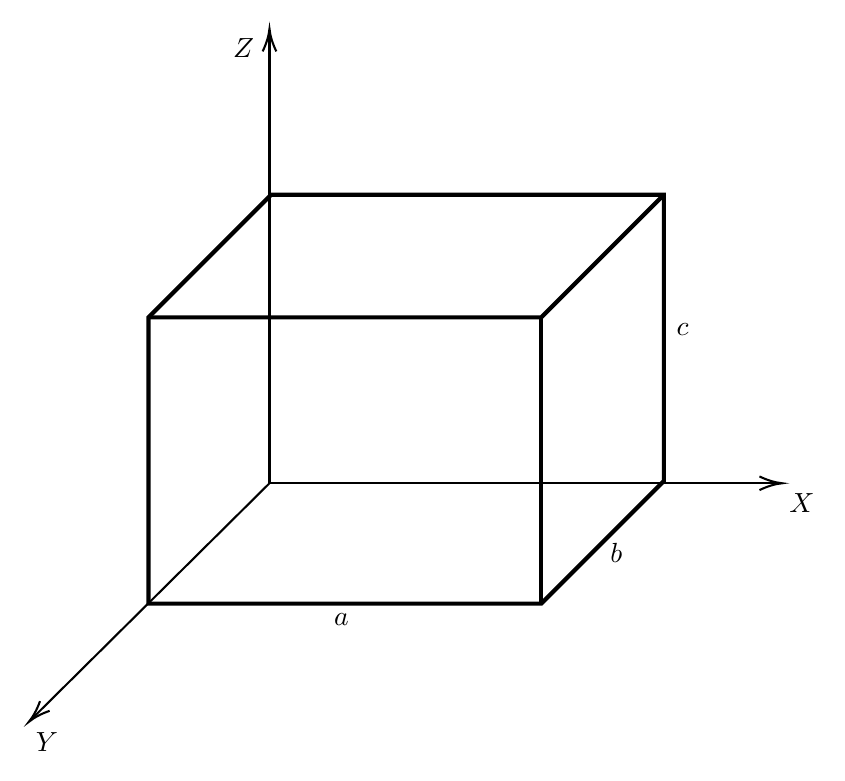
\begin{tikzpicture}[x=0.75pt,y=0.75pt,yscale=-1,xscale=1]
		%uncomment if require: \path (0,638); %set diagram left start at 0, and has height of 638
		
		%Straight Lines [id:da2805084368967936] 
		\draw    (239.3,243) -- (239.3,26) ;
		\draw [shift={(239.3,24)}, rotate = 90] [color={rgb, 255:red, 0; green, 0; blue, 0 }  ][line width=0.75]    (10.93,-3.29) .. controls (6.95,-1.4) and (3.31,-0.3) .. (0,0) .. controls (3.31,0.3) and (6.95,1.4) .. (10.93,3.29)   ;
		%Shape: Cube [id:dp7604940367971222] 
		\draw  [line width=1.5]  (181,163.1) -- (240.1,104) -- (429.3,104) -- (429.3,241.9) -- (370.2,301) -- (181,301) -- cycle ; \draw  [line width=1.5]  (429.3,104) -- (370.2,163.1) -- (181,163.1) ; \draw  [line width=1.5]  (370.2,163.1) -- (370.2,301) ;
		%Straight Lines [id:da6298786350254553] 
		\draw    (239.3,243) -- (124.72,356.59) ;
		\draw [shift={(123.3,358)}, rotate = 315.25] [color={rgb, 255:red, 0; green, 0; blue, 0 }  ][line width=0.75]    (10.93,-3.29) .. controls (6.95,-1.4) and (3.31,-0.3) .. (0,0) .. controls (3.31,0.3) and (6.95,1.4) .. (10.93,3.29)   ;
		%Straight Lines [id:da3500588708413914] 
		\draw    (239.3,243) -- (484.3,243) ;
		\draw [shift={(486.3,243)}, rotate = 180] [color={rgb, 255:red, 0; green, 0; blue, 0 }  ][line width=0.75]    (10.93,-3.29) .. controls (6.95,-1.4) and (3.31,-0.3) .. (0,0) .. controls (3.31,0.3) and (6.95,1.4) .. (10.93,3.29)   ;
		
		% Text Node
		\draw (488.3,246.4) node [anchor=north west][inner sep=0.75pt]    {$X$};
		% Text Node
		\draw (125.3,361.4) node [anchor=north west][inner sep=0.75pt]    {$Y$};
		% Text Node
		\draw (220.3,27.4) node [anchor=north west][inner sep=0.75pt]    {$Z$};
		% Text Node
		\draw (269,304.4) node [anchor=north west][inner sep=0.75pt]    {$a$};
		% Text Node
		\draw (402,270.4) node [anchor=north west][inner sep=0.75pt]    {$b$};
		% Text Node
		\draw (434,164.4) node [anchor=north west][inner sep=0.75pt]    {$c$};
		\end{tikzpicture}
		\vspace*{3mm}
		\caption[]{Three dimensional imaginary box in which the particle moves}
	\end{figure}

	The potential electric energy of the system is given by:	

	
	As in the one-dimensional case (\SeeChapter{see section Wave Quantum Physics page \pageref{quantum potential well}}), the walls of infinite potential prevent the particle from leaving the box, and the wave function is non-zero only for position vector $\vec{r}$ being inside the box. It  necessarily vanish when one of the walls is touched. The Schrödinger equation we have to solve is (\SeeChapter{see section Wave Quantum Physics page \pageref{schrodinger wave equation}}):
	
	and boundary conditions are:
	
	Notice that the Hamiltonian can be written as the sum of the Hamiltonian in each axis (we speak of the Hamiltonian operators of course!). So we have:
	
	where:
	
	Relations that we have proved the origin in details in the section of Wave Quantum Physics of this book (see page \pageref{schrodinger wave equation}).
	
	Such a form is named a "\NewTerm{separable form}\index{chemical separable form}": the Hamiltonian is the sum of individual operators $H_i$ each depending only on one variable or degree of freedom $q_i$. This form reflects the independent nature of the movements described by the variables $q_i$.
	
	Remember now that the joint probability of two independent events is the product of the individual probabilities of the two events taken separately (\SeeChapter{see section Probabilities page \pageref{joint probability}})! We therefore expect that the presence probability density in space (\SeeChapter{see section Wave Quantum Physics page \pageref{first postulate wave quantum physics}}) with a multidimensional configuration is, in the case where the Hamiltonian is of separable form, a simple individual probability density product. In fact, the separable form of the Hamiltonian permits the separation of variables on the wave function itself!

	Let us write the solutions of the Schrödinger equation under the form:
	
	of a product of three factors each depending only of one coordinated.

	Substituting this notation in the Schrödinger equation, we get without technical developments (elementary algebra):
	
	or, by dividing both sides of this equation by $\xi(x)\vartheta(y)\zeta(z)$:
	
	which is a much more aesthetic and easier to remember.
	
	This equation requires that the sum of the three terms in the left-hand side is equal to a constant in the context of a conservative system (that is what often interested chemists)! Each of these three terms depending only on one and only one variable, so that their sum is equal to a constant, it is necessary that each term is itself constant! In fact, by taking the derivative of both sides of the above equation with respect to $x$, for example, we have:
	
	meaning that equation although  must be a constant which we will denote equation (as this term expresses an energy). We then have (surprise...):
	
	Similarly, we get:
	
	Notice that each of the separate equations that we have just obtained, for the movement of the particle in the three spatial directions, is a Schrödinger equation in a one-dimensional box. Thus, the three relations previously obtained independently describe each movement in the respective $x, y, z$ directions, limited to the respective ranges:
	
	and must be respectively  solved with boundary conditions:
	
	The results obtained in the section of Wave Quantum Physics when solving the Schrödinger equation in the case of straight wells gave us directly for reminder (see page \pageref{infinite rectangular quantum well first approach}):
	
	In summary the stationary states of the particle in the three-dimensional box are specified by three positive integers quantum numbers $\lambda, \mu, \nu$. The wave function is finally:
	
	and its respective energies (eigenvalues):
	
	The variable separation technique detailed above, is applicable only because the Hamiltonian is in separable form. It comes automatically therefore the three-dimensional probability density $\vert \Psi(x,y,z) \vert^2$ is the product of probability density $\vert \xi_\lambda(x)\vert^2,\vert \vartheta_\mu(y)\vert^2,\vert \zeta_\nu(z)\vert^2$, as we had anticipated it. We also notice that the energy of movement in three dimensional space is the sum of energy movements in all three spatial directions: the independence of these three directions or degrees of freedom, implies the additivity of their energy.
	
	\subsection{Molecular Vibrations}
	We studied in the Wave Quantum Physics section the harmonic oscillator (see page \pageref{quantum harmonic oscillator}). Now it is molecular chemistry that we will use all the power of the results obtained during the study of this system.
	
	The harmonic oscillator is a model of molecular vibrations, and is represented by a type of parabolic potential as:
	
	for a diatomic molecule. But we have proved (\SeeChapter{see section Wave Mechanics page \pageref{potential energy harmonic oscillator}}) that $c^{te}=m\omega_0^2$ so that we finally have for a diatomic molecule:
	
	For a polyatomic molecule, we have verbatim (by the additivity of energy):
	
	Quantities $\omega_0$ and $\omega_i$ are the vibration frequencies (or rather more correctly: the pulsation) of a molecule, diatomic in the first case and polyatomic in the second case. In the first equation, the variable $x$ represents the elongation of the bond between the two atoms $A$ and $B$ (as with a spring) in a diatomic molecule, that is to say $x=R-R_{eq}$, where $R$ is the instantaneous length of this bond, and $R_{eq}$ is its equilibrium value.
	
	In the case of a polyatomic molecule, the potential describing molecular vibrations takes a separable form in terms of summation above only if one considers special variables $q_i$ denoting collective motions of nuclei, and which are named "\NewTerm{normal vibration modes}\index{normal vibration modes}".
	
	We also saw in the section of Wave Quantum Physics (see page \pageref{quantum harmonic oscillator}) that the Hamiltonian of a diatomic molecule (problem of the harmonic oscillator) can be written as
	
	For a polyatomic molecule that relationship becomes logically:
	
	The Hamiltonian above is clearly a type of separable form: it is a sum of one-dimensional Hamiltonians, each depending only on a single mode $q_i$ as variable, describing this mode as a unique spring or harmonic unit mass ($m=1$) oscillator and of pulse oscillation $\omega_i$. Therefore, a separation of variables $q_i$ is possible, reducing the Schrödinger time independent into a number of equations of the same type as that of a one-dimensional harmonic oscillator. So we need just to know the expression of the wave function for a one-dimensional harmonic oscillator, what we already have done in the section of Wave Quantum Physics (see page \pageref{quantum harmonic oscillator}) where we got:
	
	and:
	
	The figure below shows the graph of the first wave functions of the above relation as well as that of their respective presence probability densities. We can see the same modal structures as those specific to functions of a particle in a one-dimensional box:
	\begin{figure}[H]
		\begin{center}
		\includegraphics{img/chemistry/one_dimensionnal_oscillator.jpg}
		\end{center}	
		\caption{Wave functions and probability density of a one-dimensional harmonic oscillator}
	\end{figure}
	Above the first energy levels of a one-dimensional oscillator with \texttt{\textbf{(a)}} their associated eigenfunction, \texttt{\textbf{(b)}} the  associated probability distribution of presence.
	
	In the limit of very large values of $n$, the probability distribution approximates more and more of that predicted by classical mechanics, the oscillator lies for the most of the time in the vicinity of the turning points defined by the intersection of potential $E_{p}$ with the level of $n$. This trend is illustrated below:
	\begin{figure}[H]
		\begin{center}
		\includegraphics{img/chemistry/one_dimensionnal_oscillator_limit.jpg}
		\end{center}	
		\caption{Probability density function of a one-dimensional harmonic oscillator for large $n$}
	\end{figure}
	For a polyatomic molecule the expression of quantified energy therefore becomes:
	
	and eigenfunctions/eigenstates become:
	
	with:
	
	The last two relations are very important because they allow among others to:
	\begin{itemize}
		\item Predict the spectrum of the molecule (spectroscopy)
		\item To study the energy bands (where does the bands of valence and conduction comes from)
		\item To locate the bonds between atoms and thus the chemical properties
	\end{itemize}

	We will go further into the subject of molecular vibrations later below at page \pageref{molecular rotational energy levels} during our study of molecular vibrations energy levels that will be very important in practice to predict the spectrum of molecules (or respectively their moment of inertia).
	
	\subsection{Hydrogenoid Atom (Schrödinger model)}
	We consider here the quantification of a generic system made of two bodies (particles) interacting with each other and moving in a three-dimensional space. We will be prove at first that, even if the separation of dynamic variables describing individually each of the two bodies is impossible, for cons, the overall movement system (the center of mass) and internal movement, also said "relative motion", are separable. In addition, if the potential is centrosymmetric, the internal movement may also be decomposed into a rotational movement and radial movement. The quantification of the rotational movement is intimately connected to that of angular momentum.
	
	Here we focus on the mechanics of an atomic system having only one electron. This is a two-particle system: a nucleus of mass $M$ and charge $+Zq_e$, and an electron of mass $m_e$ and of charge $-q_e$ in the framework of the Schrödinger model (for a more generalized treatment based on Dirac equation see \cite{reiher2015relativistic}).
	
	The atomic system is described by the following Hamiltonian:
	
	Remember that in the section of Wave Quantum Physics we had proved during our study of functional operators (see page \pageref{hermitian operators of linear momentum}):
	
	and remember also that $\vec{r}_e$ and $\vec{R}_n$ are respectively the position vectors of the electron and nucleus in the prior-previous relation.
	
	The potential electric energy being given by (\SeeChapter{see section Electrostatics page \pageref{electrostatic potential energy}}):
	
	The movements of the two particles are correlated because the two charges interact through their mutual electrical field. We can not make a separation between variables $\vec{r}_e$ and $\vec{R}_N$. By cons, a separation of variables is possible with the coordinate of the center of mass (see the definition of the center of mass in the section of Classical Mechanics at page \pageref{center of mass}):
	
	and the relative coordinate of the electron relative to the nucleus:
	
	We get therefore:
	
	and:
	
	The Hamiltonian in the center of mass repository will therefore be written:
	
	where $M_{\text{tot}}=m_e+M$ is the total mass of the system and:
	
	is its reduced mass.
	
	We clearly see that the Hamiltonian $H$ is this time set in a separable form and we can write it as follows:
	
	with:
	
	In terms of the coordinates $\vec{R}_{\text{CM}}$ and $\vec{r}_{\text{rel}}$, the function describing a stationary state of the two-body system is a product of individual wave functions (recall that the joint probability of two events is the product of probabilities), one for the movement of the center of mass and the other for the relative movement:
	
	and the energy of this state is the sum of the respective energies of movements:
	
	with:
	
	\begin{tcolorbox}[title=Remark,arc=10pt,breakable,drop lifted shadow,
  skin=enhanced,
  skin first is subskin of={enhancedfirst}{arc=10pt,no shadow},
  skin middle is subskin of={enhancedmiddle}{arc=10pt,no shadow},
  skin last is subskin of={enhancedlast}{drop lifted shadow}]
	This approach of separating the wave function into the composition of a wave function of the center of mass and the relative movement is also used in the context of the study of poly-electronic atoms, but with one difference: as the nucleus is much more massive than the processing electrons (in approximation ...), the center of mass is assimilated to the nucleus of the atom and the relative motion to the entire electron cloud\index{electron cloud}\footnote{The electron cloud is the region of negative charge surrounding an atomic nucleus that is associated with an atomic orbital. The region is defined mathematically, describing a region with a high probability of containing electrons. As we know it, the electron cloud model differs from the more simplistic Bohr model, in which electrons orbit the nucleus in much the same way as planets orbit the Sun. In the cloud model, there are regions where an electron may likely be found, but it's theoretically possible for it to be located anywhere, including inside the nucleus.}. This approximate approach is well known under the designation "\NewTerm{Born-Oppenheimer approximation}\index{Born-Oppenheimer approximation}".
	\end{tcolorbox}
	Where the Hamiltonian appearing in the first of these relations has been defined above as being:
	
	This movement is that of a particle of mass $M_{\text{tot}}$ in a three-dimensional box of infinite volume. Eigenvalues and eigenfunctions for this movement has already been obtained in our previous study, we will restrict ourselves to the study of separate equation for the relative movement, or internal movement. As no confusion will be possible between different Hamiltonians, we let down, to simplify the notations, the "eel" word in subscript.
	
	With $H_{\text{rel}}$ given by the relation that we have proved previously:
	
	and the relation (as proved above):
	
	then we obtain the Schrödinger equation for the relative motion:
	
	or written differently:
	
	Notice that in the case where the potential energy $E_{p}$ is a centrosymmetric source, that is to say it depends only on the length of the position vector $\vec{r}$, and not its orientation, the previous equation, written in Cartesian coordinates, is inseparable. Indeed, in Cartesian coordinates, the length $\vec{r}$ is given by:
	
	and the potential energy can not be separated into three components, each depending only one of the three variables $x, y, z$. The Hamiltonian is therefore still not a separable form and so we did not meet our target. However, the above equation is separable at the moment we make a change of coordinates to spherical coordinates. Indeed, in this coordinate system, the potential depends on only on one of the three spherical variables: the radius $r$. It is independent of the two angles $\theta$ and $\phi$.
	
	Referring to the result obtained in the study of the Laplace expressions in different coordinate systems, in the section of Vector Calculus, we got for the Laplacian of a scalar field in spherical coordinates the following expression (see page \pageref{scalar laplacian}):
	
	The Hamiltonian:
	
	then becomes (simple distribution and new way to note):
	
	where:
	
	is the kinetic energy operator for the radial movement of the electron relative to the nucleus, and $L^2$ is the squared "associated" operator of the angular momentum vector:
	
	The term:
	
	where $J=\mu r^2$ is therefore an energy associated with the angular momentum $L$ (\SeeChapter{see section Classical Mechanics page \pageref{moment of inertia} and page \pageref{angular momentum}}).
	
	To understand the nature of this operator $L^2$ a detour by the notion of rigid rotor will help.
	
	\subsubsection{Rigid Rotator}\label{quantum chemistry rigid rotator}
	If we now consider the case of a system named "\NewTerm{rigid rotor}\index{rigid rotor}" where we neglect ("restrict" would be a more appropriate term ...) the degrees of freedom of oscillation (this is the system that are the study case for linear diatomic or polyatomic molecules), the only coordinates being into play are the angles $\theta$ and $\phi$ which fix the orientation of the rotator.
	
	Thus, in this case $r$ is fixed and we have:
	
	and in view of the constraints on the potential, it is normally quite easy to understand why the rotator is said to be "rigid". In the above case, the Hamiltonian is reduced to:
	
	
	For the rest, we associate the operator $L^2$ to the square of an angular momentum, for the simple reason that he has the units of it... Indeed, let us recall that we have prove in the section of Wave Quantum Physics that when the spin is zero (so as part of our study of the hydrogenoid atom here, the spin will not be taken into account in the first instance) and that we are dealing with a single particle then the angular momentum (which we will denote by $L$ instead of $b$) is given by:
	
	where the components of the vector $\vec{l}$ are also natural numbers. By doing this similarity, we can then write the Schrödinger equation in the form:
	
	Let us recall that we got in the section of Wave Quantum Physics that (see page \pageref{angular momentum and spin}):
	
	by the vector product.
	
	We go now to rectangular coordinates $x, y, z$ coordinates to spherical coordinates $r,\theta,\phi$. Remember for this (\SeeChapter{see section Vector Calculus page \pageref{spherical coordinates}}) that:
	
	and that:
	
	Now let us express the total differentials:
	
	These relations can be written as an orthogonal transformation of the total differential $\mathrm{d}r,r\mathrm{d}\theta,r\sin(\theta)\mathrm{d}\phi$ by:
	
	or by the inverse transformation (if required ... it is enough to check that the two transformation matrices multiplied together give the identity matrix):
	
	It results of this for example:
	
	and finally (the method for the second and third lines is the same as for the first!):
	
	Thus, taking into account these relations, we get for example, in the case of the operator:
	
	the following developments:
	
	which gives the following result:
	
	By doing the same with:
	
	and processing with the same developments:
	
	we get the following result:
	
	And for finish with:
	
	and again processing the same developments:
	
	we get the following result:
	
	Finally, we have only little freedom for the movement of our rigid rotor (as it is very rigid ...) and we can write for the Schrödinger equation:
	
	where $H_\text{rot}$ is for recall, seen as the functional linear operator, and the total energy $E$ as its corresponding eigenvector.

	Therefore, we can write that angular momentum operator is given by (we change the notation so to not confuse subsequently operator and eigenvalue according to the comments we made during the statement of the postulates of Wave Quantum Physics in the corresponding section):
	
	Thus, the eigenfunctions $\Phi(\phi)$ of $\hat{L}_z$ are solutions of the equation to the eigenvalues and eigenfunctions:
	
	that is to say the differential equation:
	
	where $L_z$ is obviously the eigenvalue of $\hat{L}_z$. A simple solution to this differential would be:
	
	with for uniformity condition, depending on the properties of complex number (\SeeChapter{see section Numbers page \pageref{complex numbers}}):
	
	This mathematical condition imposes the obvious and remarkable following quantification:
	
	where (recall) $m_l$ is the magnetic quantum number.

	Knowing that (\SeeChapter{see section Corpuscular Quantum Physics page \pageref{quantum number of orbital angular momentum interval}}):
	
	We can write:
	
	Therefore, we falls back on the result(s) that we get in the section of Corpuscular Quantum Physics and Wave Quantum Physics (see page \pageref{angular momentum and spin}):
	
	Which is quite satisfactory, even remarkable and enjoyable (to not say it ...).
	
	Thus, the measurement of one of the components of the angular momentum, provides always a multiple of $\hbar$ which appears therefore as a natural unit of angular momentum.
	
	The common eigenfunctions (!!!) to the operators $\hat{L}^2$ and $\hat{L}_z$ are in a more general framework necessarily of the form (method of separation of variables):
	
	As the rotator is rigid, we have $R(r)=c^{te}$. This factor will eliminate itself in the equation of eigenvalues and eigenfunctions that we will determine further below. So we don't need to take it into account if we want! Finally, we can write thanks to previous developments:
	
	Which brings us to the following equation of the eigenvalues and eigenfunctions:
	
	That is to say:
	
	Therefore:
	
	By putting:
	
	and therefore:
	
	we get a "Fuchs" like differential equation given by:
	
	Therefore we get finally:
	
	Whose coefficients have poles (singularities) in $\xi=\pm 1$. But, let us recall that we have:
	
	So that we often find the previous differential equation in the following form in the books after elementary algebra factorization of some terms:
	
	That is obviously also often written in the literature\label{polar equation rigid rotator}:
	
	A non-trivial solution being, assuming we know Fuchs differential equations (...), what it is customary to name the "\NewTerm{associated Legendre polynomials}\index{associated Legendre polynomials}\label{legendre polynomial}" (although this is not strictly speaking a polynomial ....) because containing partly Legendre polynomials (\SeeChapter{see section Calculus page \pageref{legendre polynomials}}):
	
	that you can check by injecting this solution in prior-previous differential equation.
	
	...Following the request of a reader here is an example of verification before continuing:
	
	The $m_l=l=0$ is immediate. Then let us consider the case where $m_l=l=1$:
	
	Thus:
	
	And we inject in it the associated Lagrange polynomial:
	
	Therefore:
	
	Which give after a small simplification:
	
	By derivating:
	
	Let's focus on the left part to see what it is equal to by putting everything to a common denominator:
	
	By simplifying the numerator, it should be zero. Let us see this by simplifying a first time:
	
	by distributing:
	
	Which is indeed equal to zero!!!
 	\begin{figure}[H]
		\centering
		\includegraphics[width=\textwidth]{img/chemistry/image_spherical_harmonics.jpg}	
		\caption{Legendre spherical harmonics plot}
	\end{figure}
	With the corresponding MATLAB™ 2013a script\footnote{It is a bit long but we really thinks it helps for a better understanding. Reader interested on how to do it with R can refer to the \texttt{R} companion book where the script is provided!} (we give the script here as it is not given in the MATLAB™ companion book) provided on Internet by Sanjay Sekaran (big thanks!):
	\begin{lstlisting}[language=MATLAB]
		theta = 0:pi/40:pi;                   % polar angle
		phi = 0:pi/20:2*pi;                   % azimuth angle
		
		[phi,theta] = meshgrid(phi,theta);    % define the grid
		
		degree = 0;
		order = 0;
		amplitude = 0.5;
		radius = 5;
		
		Ymn = legendre(degree,cos(theta(:,1)));
		Ymn = Ymn(order+1,:)';
		yy = Ymn;
		
		for kk = 2: size(theta,1)
		    yy = [yy Ymn];
		end
		
		yy = yy.*cos(order*phi);
		
		order = max(max(abs(yy)));
		rho = radius + amplitude*yy/order;
		
		r = radius.*sin(theta);    % convert to Cartesian coordinates
		x = r.*cos(phi);
		y = r.*sin(phi);
		z = radius.*cos(theta);
		
		subplot(5,5,1)
		surf(x,y,z, rho);
		title('$\ell=0, m=0$')
		
		shading interp
		
		axis equal off      % set axis equal and remove axis
		view(0,30)         % set viewpoint
		
		%%%%%%%%%%%%%%%%%%%%%%%%%%%%%%%%%%%%%%%%%%%%%%%%%%%%%%%%
		degree = 1;
		order = 0;
		amplitude = 0.5;
		radius = 5;
		
		Ymn = legendre(degree,cos(theta(:,1)));
		Ymn = Ymn(order+1,:)';
		yy = Ymn;
		
		for kk = 2: size(theta,1)
		    yy = [yy Ymn];
		end
		
		yy = yy.*cos(order*phi);
		
		order = max(max(abs(yy)));
		rho = radius + amplitude*yy/order;
		
		r = radius.*sin(theta);    % convert to Cartesian coordinates
		x = r.*cos(phi);
		y = r.*sin(phi);
		z = radius.*cos(theta);
		
		subplot(5,5,6)
		surf(x,y,z, rho);
		title('$\ell=1, m=0$')
		shading interp
		
		axis equal off      % set axis equal and remove axis
		view(0,30)         % set viewpoint
		
		%%%%%%%%%%%%%%%%%%%%%%%%%%%%%%%%%%%%%%%%%%%%%%%%%%%%%%%%
		
		degree = 1;
		order = 1;
		amplitude = 0.5;
		radius = 5;
		
		Ymn = legendre(degree,cos(theta(:,1)));
		Ymn = Ymn(order+1,:)';
		yy = Ymn;
		
		for kk = 2: size(theta,1)
		    yy = [yy Ymn];
		end
		
		yy = yy.*cos(order*phi);
		
		order = max(max(abs(yy)));
		rho = radius + amplitude*yy/order;
		
		r = radius.*sin(theta);    % convert to Cartesian coordinates
		x = r.*cos(phi);
		y = r.*sin(phi);
		z = radius.*cos(theta);
		
		subplot(5,5,7)
		surf(x,y,z, rho);
		title('$\ell=1, m=\pm 1$')
		shading interp
		
		axis equal off      % set axis equal and remove axis
		view(0,30)         % set viewpoint
		
		%%%%%%%%%%%%%%%%%%%%%%%%%%%%%%%%%%%%%%%%%%%%%%%%%%%%%%%%
		
		degree = 2;
		order = 0;
		amplitude = 0.5;
		radius = 5;
		
		Ymn = legendre(degree,cos(theta(:,1)));
		Ymn = Ymn(order+1,:)';
		yy = Ymn;
		
		for kk = 2: size(theta,1)
		    yy = [yy Ymn];
		end
		
		yy = yy.*cos(order*phi);
		
		order = max(max(abs(yy)));
		rho = radius + amplitude*yy/order;
		
		r = radius.*sin(theta);    % convert to Cartesian coordinates
		x = r.*cos(phi);
		y = r.*sin(phi);
		z = radius.*cos(theta);
		
		subplot(5,5,11)
		surf(x,y,z, rho);
		title('$\ell=2, m=0$')
		shading interp
		
		axis equal off      % set axis equal and remove axis
		view(0,30)         % set viewpoint
		
		%%%%%%%%%%%%%%%%%%%%%%%%%%%%%%%%%%%%%%%%%%%%%%%%%%%%%%%%
		
		degree = 2;
		order = 1;
		amplitude = 0.5;
		radius = 5;
		
		Ymn = legendre(degree,cos(theta(:,1)));
		Ymn = Ymn(order+1,:)';
		yy = Ymn;
		
		for kk = 2: size(theta,1)
		    yy = [yy Ymn];
		end
		
		yy = yy.*cos(order*phi);
		
		order = max(max(abs(yy)));
		rho = radius + amplitude*yy/order;
		
		r = radius.*sin(theta);    % convert to Cartesian coordinates
		x = r.*cos(phi);
		y = r.*sin(phi);
		z = radius.*cos(theta);
		
		subplot(5,5,12)
		surf(x,y,z, rho);
		title('$\ell=2, m=\pm 1$')
		shading interp
		
		axis equal off      % set axis equal and remove axis
		view(0,30)         % set viewpoint
		
		%%%%%%%%%%%%%%%%%%%%%%%%%%%%%%%%%%%%%%%%%%%%%%%%%%%%%%%%
		
		degree = 2;
		order = 2;
		amplitude = 0.5;
		radius = 5;
		
		Ymn = legendre(degree,cos(theta(:,1)));
		Ymn = Ymn(order+1,:)';
		yy = Ymn;
		
		for kk = 2: size(theta,1)
		    yy = [yy Ymn];
		end
		
		yy = yy.*cos(order*phi);
		
		order = max(max(abs(yy)));
		rho = radius + amplitude*yy/order;
		
		r = radius.*sin(theta);    % convert to Cartesian coordinates
		x = r.*cos(phi);
		y = r.*sin(phi);
		z = radius.*cos(theta);
		
		subplot(5,5,13)
		surf(x,y,z, rho);
		title('$\ell=2, m=\pm 2$')
		shading interp
		
		axis equal off      % set axis equal and remove axis
		view(0,30)         % set viewpoint
		
		%%%%%%%%%%%%%%%%%%%%%%%%%%%%%%%%%%%%%%%%%%%%%%%%%%%%%%%%
		
		degree = 3;
		order = 0;
		amplitude = 0.5;
		radius = 5;
		
		Ymn = legendre(degree,cos(theta(:,1)));
		Ymn = Ymn(order+1,:)';
		yy = Ymn;
		
		for kk = 2: size(theta,1)
		    yy = [yy Ymn];
		end
		
		yy = yy.*cos(order*phi);
		
		order = max(max(abs(yy)));
		rho = radius + amplitude*yy/order;
		
		r = radius.*sin(theta);    % convert to Cartesian coordinates
		x = r.*cos(phi);
		y = r.*sin(phi);
		z = radius.*cos(theta);
		
		subplot(5,5,16)
		surf(x,y,z, rho);
		title('$\ell=3, m=0$')
		shading interp
		
		axis equal off      % set axis equal and remove axis
		view(0,30)         % set viewpoint
		
		%%%%%%%%%%%%%%%%%%%%%%%%%%%%%%%%%%%%%%%%%%%%%%%%%%%%%%%%
		
		degree = 3;
		order = 1;
		amplitude = 0.5;
		radius = 5;
		
		Ymn = legendre(degree,cos(theta(:,1)));
		Ymn = Ymn(order+1,:)';
		yy = Ymn;
		
		for kk = 2: size(theta,1)
		    yy = [yy Ymn];
		end
		
		yy = yy.*cos(order*phi);
		
		order = max(max(abs(yy)));
		rho = radius + amplitude*yy/order;
		
		r = radius.*sin(theta);    % convert to Cartesian coordinates
		x = r.*cos(phi);
		y = r.*sin(phi);
		z = radius.*cos(theta);
		
		subplot(5,5,17)
		surf(x,y,z, rho);
		title('$\ell=3, m=\pm 1$')
		shading interp
		
		axis equal off      % set axis equal and remove axis
		view(0,30)         % set viewpoint
		
		%%%%%%%%%%%%%%%%%%%%%%%%%%%%%%%%%%%%%%%%%%%%%%%%%%%%%%%%
		
		degree = 3;
		order = 2;
		amplitude = 0.5;
		radius = 5;
		
		Ymn = legendre(degree,cos(theta(:,1)));
		Ymn = Ymn(order+1,:)';
		yy = Ymn;
		
		for kk = 2: size(theta,1)
		    yy = [yy Ymn];
		end
		
		yy = yy.*cos(order*phi);
		
		order = max(max(abs(yy)));
		rho = radius + amplitude*yy/order;
		
		r = radius.*sin(theta);    % convert to Cartesian coordinates
		x = r.*cos(phi);
		y = r.*sin(phi);
		z = radius.*cos(theta);
		
		subplot(5,5,18)
		surf(x,y,z, rho);
		title('$\ell=3, m=\pm 2$')
		shading interp
		
		axis equal off      % set axis equal and remove axis
		view(0,30)         % set viewpoint
		
		%%%%%%%%%%%%%%%%%%%%%%%%%%%%%%%%%%%%%%%%%%%%%%%%%%%%%%%%
		
		degree = 3;
		order = 3;
		amplitude = 0.5;
		radius = 5;
		
		Ymn = legendre(degree,cos(theta(:,1)));
		Ymn = Ymn(order+1,:)';
		yy = Ymn;
		
		for kk = 2: size(theta,1)
		    yy = [yy Ymn];
		end
		
		yy = yy.*cos(order*phi);
		
		order = max(max(abs(yy)));
		rho = radius + amplitude*yy/order;
		
		r = radius.*sin(theta);    % convert to Cartesian coordinates
		x = r.*cos(phi);
		y = r.*sin(phi);
		z = radius.*cos(theta);
		
		subplot(5,5,19)
		surf(x,y,z, rho);
		title('$\ell=3, m=\pm 3$')
		shading interp
		
		axis equal off      % set axis equal and remove axis
		view(0,30)         % set viewpoint
		
		%%%%%%%%%%%%%%%%%%%%%%%%%%%%%%%%%%%%%%%%%%%%%%%%%%%%%%%%
		
		degree = 4;
		order = 0;
		amplitude = 0.5;
		radius = 5;
		
		Ymn = legendre(degree,cos(theta(:,1)));
		Ymn = Ymn(order+1,:)';
		yy = Ymn;
		
		for kk = 2: size(theta,1)
		    yy = [yy Ymn];
		end
		
		yy = yy.*cos(order*phi);
		
		order = max(max(abs(yy)));
		rho = radius + amplitude*yy/order;
		
		r = radius.*sin(theta);    % convert to Cartesian coordinates
		x = r.*cos(phi);
		y = r.*sin(phi);
		z = radius.*cos(theta);
		
		subplot(5,5,21)
		surf(x,y,z, rho);
		title('$\ell=4, m=0$')
		shading interp
		
		axis equal off      % set axis equal and remove axis
		view(0,30)         % set viewpoint
		
		%%%%%%%%%%%%%%%%%%%%%%%%%%%%%%%%%%%%%%%%%%%%%%%%%%%%%%%%
		
		degree = 4;
		order = 1;
		amplitude = 0.5;
		radius = 5;
		
		Ymn = legendre(degree,cos(theta(:,1)));
		Ymn = Ymn(order+1,:)';
		yy = Ymn;
		
		for kk = 2: size(theta,1)
		    yy = [yy Ymn];
		end
		
		yy = yy.*cos(order*phi);
		
		order = max(max(abs(yy)));
		rho = radius + amplitude*yy/order;
		
		r = radius.*sin(theta);    % convert to Cartesian coordinates
		x = r.*cos(phi);
		y = r.*sin(phi);
		z = radius.*cos(theta);
		
		subplot(5,5,22)
		surf(x,y,z, rho);
		title('$\ell=4, m=\pm 1$')
		shading interp
		
		axis equal off      % set axis equal and remove axis
		view(0,30)         % set viewpoint
		
		%%%%%%%%%%%%%%%%%%%%%%%%%%%%%%%%%%%%%%%%%%%%%%%%%%%%%%%%
		
		degree = 4;
		order = 2;
		amplitude = 0.5;
		radius = 5;
		
		Ymn = legendre(degree,cos(theta(:,1)));
		Ymn = Ymn(order+1,:)';
		yy = Ymn;
		
		for kk = 2: size(theta,1)
		    yy = [yy Ymn];
		end
		
		yy = yy.*cos(order*phi);
		
		order = max(max(abs(yy)));
		rho = radius + amplitude*yy/order;
		
		r = radius.*sin(theta);    % convert to Cartesian coordinates
		x = r.*cos(phi);
		y = r.*sin(phi);
		z = radius.*cos(theta);
		
		subplot(5,5,23)
		surf(x,y,z, rho);
		title('$\ell=4, m=\pm 2$')
		shading interp
		
		axis equal off      % set axis equal and remove axis
		view(0,30)         % set viewpoint
		
		%%%%%%%%%%%%%%%%%%%%%%%%%%%%%%%%%%%%%%%%%%%%%%%%%%%%%%%%
		
		degree = 4;
		order = 3;
		amplitude = 0.5;
		radius = 5;
		
		Ymn = legendre(degree,cos(theta(:,1)));
		Ymn = Ymn(order+1,:)';
		yy = Ymn;
		
		for kk = 2: size(theta,1)
		    yy = [yy Ymn];
		end
		
		yy = yy.*cos(order*phi);
		
		order = max(max(abs(yy)));
		rho = radius + amplitude*yy/order;
		
		r = radius.*sin(theta);    % convert to Cartesian coordinates
		x = r.*cos(phi);
		y = r.*sin(phi);
		z = radius.*cos(theta);
		
		subplot(5,5,24)
		surf(x,y,z, rho);
		title('$\ell=4, m=\pm 3$')
		shading interp
		
		axis equal off      % set axis equal and remove axis
		view(0,30)         % set viewpoint
		
		%%%%%%%%%%%%%%%%%%%%%%%%%%%%%%%%%%%%%%%%%%%%%%%%%%%%%%%%
		
		degree = 4;
		order = 4;
		amplitude = 0.5;
		radius = 5;
		
		Ymn = legendre(degree,cos(theta(:,1)));
		Ymn = Ymn(order+1,:)';
		yy = Ymn;
		
		for kk = 2: size(theta,1)
		    yy = [yy Ymn];
		end
		
		yy = yy.*cos(order*phi);
		
		order = max(max(abs(yy)));
		rho = radius + amplitude*yy/order;
		
		r = radius.*sin(theta);    % convert to Cartesian coordinates
		x = r.*cos(phi);
		y = r.*sin(phi);
		z = radius.*cos(theta);
		
		subplot(5,5,25)
		surf(x,y,z, rho);
		title('$\ell=4, m=\pm 4$')
		shading interp
		
		axis equal off      % set axis equal and remove axis
		view(0,30)         % set viewpoint
		
		%%%%%%%%%%%%%%%%%%%%%%%%%%%%%%%%%%%%%%%%%%%%%%%%%%%%%%%%
		
		map = makeColorMap([0.2 0.2 0.6],[1.0 0.99 0.72],[0.8 0.25 0.33],80);
		colormap(map);
		cd(Figures)
	\end{lstlisting}
	
	So finally, we have common eigen functions (because remember that the Legendre polynomials are orthogonal to each other) that will be:
	 
	\begin{tcolorbox}[title=Remark,arc=10pt,breakable,drop lifted shadow,
  skin=enhanced,
  skin first is subskin of={enhancedfirst}{arc=10pt,no shadow},
  skin middle is subskin of={enhancedmiddle}{arc=10pt,no shadow},
  skin last is subskin of={enhancedlast}{drop lifted shadow}]
	There is no need to make complicated calculations to determine the normalization factor of the exponential, as in the context of an integration over all space, the three factors of $Y_{m_l,l}(\theta,\phi)$ are independent of each other. Thus the integral is the product of the integrals (\SeeChapter{see section Differential and Integral Calculus page \pageref{integral calculus}}).
	\end{tcolorbox}
	Finally, we must find $N_{m_l,l}$ such that:
	
	and we will see (what we will prove just below) that:
	
	In summary, we write (we should rather say "we will write"...):
	
	where we have omitted the factor $(-1)^l$ since in any case this term in the module of this function this term multiplies himself and then gives $(-1)^{2l}=1$.

Let us check now the framed previous boxed relation (warning this is a bit long and it is advisable to read it several times):

	We consider the functions defined by:
	
	where:
	
	with:
	
	The aim will therefore be to prove that these functions are orthogonal first and then find the constants $N_{m_l,l}$ such that $||Y_{m_l,l}\|$. In short we will have to roll up the sleeves... of our brain...

	First, let us prove for future needs that:
	
	\begin{dem}
	If and only if $l=m_l=0$ the equality is obvious. Let us suppose that $l\geq 1$ (thus the general case outside the obvious previous case) and given $P$ a real polynomial of degree $\leq l-1$.

	Let us put:
	
	Let us prove (functional dot product):
	
	in  $\mathcal{C}(x\in[-1,1],\mathbb{R})$.
	
	Indeed, let us recall that we made the change of variable:
	
	Integrating by parts, we get:
	
	let us notice that for any $0\leq j\leq m_l-1$, $\dfrac{\mathrm{d}^j}{\mathrm{d}x^j}Z(x)$ is equal to zero in $x=\pm 1$ that is to say:
	
	Therefore (by extension), the above relation simplifies to:
	
	After $m_l$ integration by parts equation, we get:
	
	If $\deg(P)<m_l$ then the above expression shows that trivially:
	
	If $\deg(P)\geq m_l$ then by putting:
	
	We get:
	
	let us notice once again that $\dfrac{\mathrm{d}^j}{\mathrm{d}x^j}h(x)$ vanishes in $x=\pm 1$ for any $j\leq m_l-1$, that is say:
	
	By integrating by parts $m_l$the previous expression, we find:
	
	but $h$ is a polynomial of degree $m_l+\text{deg}(P)$.
	
	Indeed, the first factor is of degree $2m$ and the $m_l$th derivative of $P(x)$" is of degree $P-m_l$, therefore:
	
	So $\dfrac{\mathrm{d}^{m_l}}{\mathrm{d}x^{m_l}}h(x)$ is a polynomial of degree $\deg(P)\leq l-1$ and knowing that $\dfrac{\mathrm{d}^l}{\mathrm{d}x^l}(1-x^2)^l$ is to a given constant equal to the $l$-th Legendre polynomial (\SeeChapter{see section Calculus page \pageref{legendre polynomials}}) we then have:
	
	So we have just proved that $\dfrac{\mathrm{d}m_l}{\mathrm{d}x^{m}_l}$ is orthogonal to any polynomial of degree $\leq l-1$.
	\begin{flushright}
		$\blacksquare$  Q.E.D.
	\end{flushright}
	\end{dem}
	$\dfrac{\mathrm{d}^{m_l}}{\mathrm{d}x^{m_l}}Z$ is a polynomial of degree $l$ (its just enough to check for some values) so therefore let us search if there is a constant $c^{te}\in\mathbb{R}$ such that:
	
	with for recall:
	
	We can determine the constant $c^{te}$ by comparing the dominant coefficients of the polynomials:
	
	The dominant coefficient of $\dfrac{\mathrm{d}^{m_l}}{\mathrm{d}x^{m_l}}Z$ is:
	
	and the dominant coefficient of $\dfrac{\mathrm{d}^l}{\mathrm{d}x^l}(1-x^2)^l$ is:
	
	Therefore:
	
	That is to say:
	
	So we would have for $l\geq m_l\geq 0$ (we integrate parts we integrate as many times as necessary to the left and right - necessarily - to achieve this result):
	
	Now let us establish a remarkable relation that should perhaps exist between $P_{-m_l,l}$ and $P_{m_l,l}$ (and which will be useful to us later). Let us assume for this $0\leq m_l\leq l$ and remember that at the base:
	
	So that brings us to write (nothing special):
	
	By the previous results ($(-1)^{m_l}=(-1)^{-m_l}$):
	
	this leads us to write:
	
	Therefore we get:
	
	
	First, let us prove that:
	
	where $P_l$ is the $n$-th Legendre polynomial (hence the origin of the name of "associated  Legendre polynomial" ...).
	\begin{dem}
	First, we have proved that the Legendre polynomials satisfy the following recurrence relation (\SeeChapter{see section Calculus page \pageref{legendre polynomials}}):
	
	for $n\geq 1$.
	Multiplying the above equation by $x^{n-1}$ and integrating, we get:
	
	But:
	
	Let us recall that the $P_{n+1}$ polynomials form an orthogonal basis of which the polynomials that generate it are of increasing degree from $0$ to $n$, so a lower order polynomial - expressed in a sub vector space - will always be perpendicular to the vectors (polynomials) generating the higher dimensions. So if we take the example of $\mathbb{R}^3$ generated by the basis $(\vec{e}_1,\vec{e}_2,\vec{e}_3)$, then a vector $\vec{v}$ expressed by the linear combination of $(\vec{e}_1,\vec{e}_2)$ will always be perpendicular to $\vec{e}_3$ and therefore a zero scalar product with it.

	And  therefore it follows:
	
	Let us put:
	
	The previous expression becomes (remember $P_0(x)=1$):
	
	Thus by induction:
	
	Furthermore as:
	
	We then have for the prior-previous relation the denominator which can obviously be rewritten:
	
	Then we have:
	
	So in the end we can simplify the denominator as follows:
	
	and:
	
	So we have well proved that (just in case ... you would not follow anymore the initial target ...) that:
	
	\begin{flushright}
		$\blacksquare$  Q.E.D.
	\end{flushright}
	\end{dem}
	Let us attack us finally to what interests us. That is to say, prove that:
	
	\begin{dem}
	If $m_l\neq j$ then:
	
	where:
	
	\begin{tcolorbox}[title=Remark,arc=10pt,breakable,drop lifted shadow,
  skin=enhanced,
  skin first is subskin of={enhancedfirst}{arc=10pt,no shadow},
  skin middle is subskin of={enhancedmiddle}{arc=10pt,no shadow},
  skin last is subskin of={enhancedlast}{drop lifted shadow}]
	Let us recall that the Jacobian in spherical coordinates is $r^2\sin(\theta)$ (\SeeChapter{see section Differential and Integral Calculus page \pageref{jacobian spherical coordinates}}) and as the integrated function above is not dependent on $r$, we have take out the term $r^2\mathrm{d}r$ of this integral (by cons we will meet again the same term in the function $R(r)$ present in the Schrödinger equation).
	\end{tcolorbox}
	And with:
	
	If $l>k$ and $m_l=j$ then the dot product of:
	
	is simplified to:
	
	By doing the change of variable $x=\cos(\theta)$ we get:
	
	Let us suppose that $m_l\geq 0$:
	
	where $P_l(x)$ is the $n$-th Legendre polynomial. Thus the expression of the dot product becomes:
	
	If we put:
	
	then the relation becomes:
	
	Integrating by parts $m$ times the expression above we get:
	
	But $\dfrac{\mathrm{d}^{m_l}}{\mathrm{d}x^{m_l}}h(x)$ is a polynomial of degree $k$. Knowing that $l>k$, the latter integral is zero for the same reasons as those mentioned above. Therefore:
	
	If $m_l<$ then we have proved that:
	
	and therefore:
	
	as $-m_l\geq 0$.
	
	It only remains to us to treat the case $m_l=j,l=k$. Let us suppose again that $m_l\geq 0$. So as before we have:
	
	and:
	
	Let us put:
	
	The relation then becomes:
	
	By integrating $m$ times by parts, we find:
	
	$\dfrac{\mathrm{d} ^{m_l}}{\mathrm{d} x^{m_l}}h(x)$ is a polynomial of degree $l$ which dominant coefficient is equal to:
	
	$P_l$ being orthogonal to any polynomial of degree strictly less that $l$, the expression can be written:
	
	But, we have proved that:
	
	therefore:
	
	If $m_l\leq 0$ we know that we get the result.
	\begin{flushright}
		$\blacksquare$  Q.E.D.
	\end{flushright}
	\end{dem}
	Finally this result gives us also the normalization condition:
	
	And so finally:
	
	is indeed an orthonormal family. Either explicitly (we reintroduce the factor $(-1)^l$):
	
	Finally, after this highly mathematical interlude (but instructive for the methodology of approach), we see (which is logical) that to each value of $l$ correspond therefore $2l + 1$ eigenfunctions $Y_{m_l,l}(\theta,\phi)$. We also say that the value $\hbar l(l+1)$ is $2l + 1$ times degenerated since:
	
	Here are some values of the function  $Y_{m_l,l}(\theta,\phi)$ (here below denoted $Y_{l}^{m_l}(\theta,\phi)$) that generates what we commonly name "\NewTerm{spherical harmonics}\index{spherical harmonics}"\footnote{A special thanks to the authors of the following Wikipedia page \url{https://en.wikipedia.org/wiki/Table_of_spherical_harmonics} and we recommend by the way to take a close look to the \textit{Talk} tab of this page!}. Some of these formulas give the "Cartesian" version (useful for some softwares that doesn't manage directly plots in spherical coordinates...). This assumes $x$, $y$, $z$, and $r$ are related to $\theta$  and $\phi$ through the usual spherical-to-Cartesian coordinate transformation (\SeeChapter{see section Vector Calculus page \pageref{spherical coordinates}}):
	
	So let's start!:
	
	
	
	
	
	
	
	
	
	
	
	
	Let's see some plots of these beautiful spherical harmonics that can be obtained with Maple 4.00b\footnote{For the \texttt{R} equivalent code, the reader can refer to the \texttt{R} companion book} by using the following command (this is the $Y_2^{-1}(\theta,\phi)$ spherical harmonic function above):\\

	\texttt{>plot3d(Re(-sqrt(15/(8*Pi))*(sin(theta)*cos(theta)*exp(-I*phi)))\string^2,phi=0..2*Pi,\\theta=0..Pi, coords=spherical,scaling=constrained,numpoints=5000,axes=frame);}
	\begin{figure}[H]
		\centering
		\includegraphics{img/chemistry/orbit_rigid_rotator_hydrogen_y12_maple.jpg}	
		\caption{Plot of the spherical harmonics $Y_{1,2}$}
	\end{figure}
	
	\begin{itemize}
		\item $Y_{0,0}$ (corresponding to $n=1$!) gives a sphere (constant value regardless $\theta,\phi$) which the probability density can be represented by the following "\NewTerm{photographic card}\index{photographic card (chemistry)}" or "\NewTerm{density map}\index{density map (chemistry)}" (the density in a given state is represented by the density of light spotted on a dark background):
		\begin{figure}[H]
			\centering
			\includegraphics{img/chemistry/density_map1s.jpg}	
			\caption{$1s$ density map}
		\end{figure}
		Representing the possible $1s$ orbits.

		\item $Y_{0,1},Y_{1,1},Y_{-1,1}$ give (for $n=2$  at least!):
		\begin{figure}[H]
			\centering
			\includegraphics{img/chemistry/harmonic_functions_2p.jpg}	
			\caption{$2p$ orbitals (spherical harmonics)}
		\end{figure}
		Which represents the possible $2p$ orbits, the probability density function can be represented by its density and isodensity maps:
		\begin{figure}[H]
			\centering
			\includegraphics{img/chemistry/density_map2p.jpg}	
			\caption{$2p$ density map}
		\end{figure}

		\item $Y_{-2,2},Y_{-1,2},Y_{1,2},Y_{2,2},Y_{0,2}$ give (for $n=3$  at least!):
		\begin{figure}[H]
			\centering
			\includegraphics{img/chemistry/harmonic_functions_3d.jpg}	
			\caption{$3d$ orbitals (spherical harmonics)}
		\end{figure}
		Representing $5$ possible $3d$ centrosymmetric  orbits, which the probability density can be represented by (the last two maps represent $Y_{0,2}$) the following density maps:
		\begin{figure}[H]
			\centering
			\includegraphics{img/chemistry/density_map3d.jpg}	
			\caption{$3d$ density map}
		\end{figure}

		\item $Y_{-3,3},Y_{-2,3},Y_{-1,3},Y_{1,3},Y_{2,3},Y_{3,3},Y_{0,3}$ give (for $n=4$  at least!):
		\begin{figure}[H]
			\centering
			\includegraphics{img/chemistry/harmonic_functions_4f.jpg}	
			\caption{$3d$ orbitals (spherical harmonics)}
		\end{figure}
		Representing $7$ possible $3f$ anti-centrosymmetric  orbits, which the probability density can be represented by (in the order: $Y_{0,3},Y_{\pm 1,3},Y_{\pm 2,3},Y_{\pm 3,3}$) the following density maps:
		\begin{figure}[H]
			\centering
			\includegraphics{img/chemistry/density_map4f.jpg}	
			\caption{$4f$ density map}
		\end{figure}
	\end{itemize}
	Or in a much better quality (from top-left to bottom right we have $Y_0^0, Y_1^{-1},Y_1^0,Y_1^1,Y_2^{-2},Y_2^{-1},Y_2^{0},Y_2^1,Y_2^2,Y_3^0$):
	\begin{figure}[H]
		\centering
		\includegraphics{img/chemistry/spherical_harmonics.pdf}	
		\caption[]{3d orbitals (spherical harmonics) made with TikZ (author: Jeff Hein)}
	\end{figure}
	The above results thus lead us to write:
	
	Substituting this in the Schrödinger equation:
	
	We get ($T_r=0$ in the rigid rotor but $\neq 0$ in the case of the hydrogen atom):
	
	As there is in this relation no operator which acts on $Y_{m_l,l}(\theta,\phi)$, we can simplify to obtain:
	
	which we see in the general case of the isolated atom that energy levels are no longer dependent of $m_l$ (due to the spherical symmetry of the potential). Then we say that the levels corresponding to the same values of $n$ and of $l$ are all merged whatever the values of $m_l$.
	
	In the case where $E_p$ derived from the $1 / r$ Coulomb potential , this radial equation leads us to a normalizing solution of $R (r)$ (different from zero then...) only for values of the energy corresponding to the following quantization law (well ... what a coincidence, we fall back on the expression proved in the old models of Corpuscular Quantum Physics at page \pageref{Rydberg constant}!):
	
	where $R_H$ is the Rydberg constant as we determined in the section of Corpuscular Quantum Physics. Thus, in this case the energy levels corresponding to the same values of $n$ are all merged regardless of the value of $l$.

	Remember that from the beginning we assume a rigid rotator with $R(r)=c^{te}$. And what if we consider now the non-rigid version?
	
	\subsubsection{Non-Rigid Rotator}\label{quantum chemistry non-rigid rotator}
	Let us remind that we started from:
	
	Or more explicitly:
	
	Therefore in polar coordinates:
	
	Both LHS and RHS contain a term linear in $\Psi$, so combine:
	
	Using the separation of variables idea, we assume a product solution of a radial and an angular function:
	
	Since $Y$ does not depend on $r$, we can move it in front of the radial derivative:
	
	and, similarly, $R$ does not depend on the angular variables. Thus replace $\Psi$ and the differentials:
	
	We multiply by $r^2$ and divide by $RY$ to separate the radial and angular terms:
	
	The first and fourth terms depend on $r$ only, the middle terms depend on the angles only. They can only balance each other for all points in space if the radial and angular terms are the same constant but with opposite sign.
	
	Therefore, we can separate into a radial equation:
	
	and an angular equation:
	
	where $A$ is the separation constant.
	
	The angular part still contains terms depending on both $\theta$ and $\phi$. Another separation of variables is needed.
	
	We'll replace $Y$ by a product of single-variable functions:
	
	And we just see earlier what it took us to! However let us continue because we would like to know the value of $A$!
	
	Replacing $Y$ and the differentials, we have:
	
	Isolating variables in separate terms:
	
	With $B$ as separation constant, we have a polar part:
	
	where $B$ is another separation constant! Rearranging we get:
	
	And here we recognize something known to us. We already proved earlier (see page \pageref{polar equation rigid rotator}):
	
	So we can immediately associate $A=l(l+1)$ and $B=m_l$. Great!
	
	That means now we can write the radial equation as:
	
	We apply the product rule to the first term:
	
	and divide by $r^2$:
	
	We can't solve this straight away, but for very large $r$, the highlighted terms are forced to zero because they go reciprocal with $r$.
	
	That leaves us with an asymptotic equation:
	
	which is another ordinary differential equation with constant coefficients. Having for solution:
	
	
	It makes sense to use as the zero point of potential energy the energy of a free electron, i.e. in this asymptotic case, $E \rightarrow 0$ for an electron far away from the nucleus, as it is practically free. Since the presence of the positive charge in the nucleus stabilises the atom, we must look for solutions where $E$ becomes negative as the electron comes closer to the nucleus. These two conditions are met if we choose $C_{2}=0$ and use the fact that $E<0$ to get rid of the imaginary unit.
	
	The asymptotic solution is then:
	
	For bound states, $R \rightarrow 0$ as $r \rightarrow +\infty$, and $R$ is finite at the origin, $r=0$. We do not consider continuum states with positive energy. Only when the latter are included do hydrogen wave functions form a complete set.
	
	By use of the abbreviations (resulting from rescaling $r$ to the dimensionless radial variable $\rho$):
	
	the equation:
	
	becomes:
	
	where $\chi(\rho)=R(\rho / \alpha)$. A comparison with the differential equation introduced during our study of Laguerre polynomials in the section of Calculus page \pageref{radial term dimensionless non-rigid rotator} for $\Phi_{n}^{k}(x)$ (with a small change in the notation):
	
	 shows that the previous relation is satisfied by:
	
	in which $k$ is replaced by $2 l+1$ (as $(k^2-1)/4=l(l+1)$) and $j$ by $\lambda-l-1$, upon using:
	
	We must restrict the parameter $\lambda$ by requiring it to be an integer $n, n=1,2,3, \ldots$. This is necessary because the Laguerre function of non-integral $n$ would diverge as $\rho^{n} e^{\rho}$, which is unacceptable for our physical problem, in which:
	
	This restriction on $\lambda$, imposed by our boundary condition, has the effect of quantizing the energy! 
	
	The comparison of the two ordinary differential equations above gives us the eigenenergies of the hydrogen atom, but require some development. Since $k=2 l+1$:
	
	From the discussion on associated Laguerre polynomials, the indices $j$ and $k$ are non-negative. The sum $j+l+1$ can, therefore, assume any integer values of $1$ or greater. We are going to rename it $n$, or:
	
	The new integer index $n$ is known as the principal quantum number. Using the principal quantum number, we can deduce the eigenenergies of the hydrogen atom. Indeed we have comparing again the two ordinary differential equations:
	
	Squaring:
	
	and simplifying by injecting again $\alpha$ leads us to:
	
	where $r_0$ is the Bohr radius given for reminder by:
	
	Now coming back to:
	
	Let us explicit it:
	
	Using:
	
	Therefore:
	
	After simplifying a bit and rearranging:
	
	Finally adding a normalization constant\footnote{Derive or even check that the normalization constant is the right one takes between five to ten pages so we will do that in the future when we will have the time to write a lot of \LaTeX ...}:
	
	
	For a given value of the principal quantum number $n$ (recall that we saw in the section of Corpuscular Quantum Physics at page \pageref{quantum number of orbital angular momentum} that $l\leq n-1$), it is possible to verify that there are several solutions to the function $R(r)$ according to the value of the azimuthal quantum number $l$. Hence the identification of the solutions by the pair $(n, l)$. We denote them $R_{n,l}(r)$. These are real functions of the variable $r$ (it is just enough to check ... because if they work then they satisfy the Schrödinger equation, we will make an example a little further below)\label{atomic orbitals of hydrogen atom}:
	
	where (beware some books give this value in natural units!):
	
	is as we know the equivalent of the Bohr radius (for the reduced mass) that we have determined in the section of Corpuscular Quantum Physics  with the difference that here we have a reduced mass instead of a single mass.
	
	However let us see if our Schrödinger equation is satisfied (taking $n=1,l=0$ for example):
	
	Which corresponds well to the expected result.

	Which graphically gives us the radial part $R_{n,l}(r)$:
	\begin{figure}[H]
		\centering
		\includegraphics{img/chemistry/radial_functions.jpg}	
		\caption{Plot of few radial functions $R_{n,l}(r)$}
	\end{figure}
	Let us study a little more in detail the radial function in the case of the hydrogen atom!:

	In the case of the atomic orbital $1s$ (!special case but we could do the same calculations as the following with all other orbital!) we have for the hydrogen atom:
	
	So it is well a decreasing exponential function as shown in the graphic above. Before continuing let us recall that (\SeeChapter{see section Wave Quantum Physics page \pageref{first postulate wave quantum physics}}) :
	
	But, in spherical coordinates (see the beginning of this section):
	
	It then comes as we have seen earlier above:
	
	Then it follows that:
	
	With this result we can calculate the radial probability of finding the electron on each atomic orbital! So, it comes immediately with the previous result:
	
	So in the case of our $1s$ atomic orbital:
	
	It is now super interesting to calculate the point $r$ point where the probability of finding the electron is maximum on the $1s$ orbital!

	For this, we notice that $\dfrac{P_r}{\mathrm{d}r}$ reaches a maximum when we have trivially:
	
	Therefore:
	
	Hence:
	
	Which is remarkable, because we fall back on the result of the Bohr model (\SeeChapter{see section Corpuscular Physics page \pageref{bohr model}})!!!
	
	\begin{tcolorbox}[title=Remark,arc=10pt,breakable,drop lifted shadow,
  skin=enhanced,
  skin first is subskin of={enhancedfirst}{arc=10pt,no shadow},
  skin middle is subskin of={enhancedmiddle}{arc=10pt,no shadow},
  skin last is subskin of={enhancedlast}{drop lifted shadow}]
	Notice that if we had kept $Z\neq 1$ then the result would have been of the shape: $r=r_0/Z$. That means more we have electrons, more these latter can be near the nucleus. We then say that the electrons screen each other somewhat from the nucleus.\label{electron screening}
	\end{tcolorbox}

	To summarize a little all this, the stationary states of the hydrogen atom are specified by three quantum numbers $n\in\mathbb{N}^{*},l\leq n-1,|m_l|\leq l$ and the Schrödinger wave function given finally by:
	
	We then have the following traditional nomenclature in the case of the hydrogen atom:
	\begin{table}[H]
	\begin{center}
		\definecolor{gris}{gray}{0.85}
			\begin{tabular}{|c|c|c|c|c|}
				\hline
				\multicolumn{1}{c}{\cellcolor[gray]{0.75}\textbf{$n$}} & 
  \multicolumn{1}{c}{\cellcolor[gray]{0.75}\textbf{$l$}} & 
  \multicolumn{1}{c}{\cellcolor[gray]{0.75}\textbf{$m_l$}}  & 
  \multicolumn{1}{c}{\cellcolor[gray]{0.75}Function} & 
  \multicolumn{1}{c}{\cellcolor[gray]{0.75}Nomenclature}\\ \hline
				1 & 0 & 0 & $\Psi_{1,0,0}$ & $1s$\\ \hline
				   &  &  &  & \\ \hline
				2 & 0 & 0 & $\Psi_{2,0,0}$ & $2s$\\ \hline
				   & 1 & 1 & $\Psi_{2,1,1}$ & $2p_1$\\ \hline
				   &   & 0 & $\Psi_{2,1,0}$ & $2p_0$\\ \hline
				   &   & -1 & $\Psi_{2,1,-1}$ & $2p_{-1}$\\ \hline
				   &  &  &  & \\ \hline
				3 & 0 & 0 & $\Psi_{3,0,0}$ & $3s$\\ \hline
				   & 1 & 1 & $\Psi_{3,1,1}$ & $3p_1$\\ \hline
				   &   & -1 & $\Psi_{3,1,-1}$ & $3p_{-1}$\\ \hline
				   &  2 & 2 & $\Psi_{3,2,2}$ & $3d_2$\\ \hline
				   &     & 1 & $\Psi_{3,2,1}$ & $3d_1$\\ \hline
				   &     & 0 & $\Psi_{3,2,0}$ & $3d_0$\\ \hline
				   &     & -1 & $\Psi_{3,2,-1}$ & $3d_{-1}$\\ \hline
				   &     & -2 & $\Psi_{3,2,-2}$ & $3d_{-2}$\\ \hline

		\end{tabular}
	\end{center}
	\caption{Nomenclature of layers and sub-layers of the hydrogen atom}
	\end{table}
	We can include the spin of the electron in the description of the electronic structure of the atom. If we treat the spin as an additional degree of freedom then the lack of interaction term between conventional degrees of freedom (positions in real space) and the spin interaction named "\NewTerm{spin-orbit coupling}\index{spin-orbit coupling}" in the previous Hamiltonian implies that we can write the total wave function, spin included, in the form of a product:
	
	
	So taking into account everything seen so far we have the following density plots:
	\begin{figure}[H]
		\centering
		\includegraphics[scale=0.8]{img/chemistry/hydrogen_full_wave_function.jpg}	
	\end{figure}
	
	where we added the spin quantum number $m_s=\pm 1/2$ (\SeeChapter{see section Corpuscular Quantum Physics page \pageref{spin}}).

	The same remark we made in the section of Corpuscular Quantum Physics then applies: the levels remain $2n^2$ times degenerated.

	Let us do an example! So we have:
	
	Thus for $1$ proton:
	
	This wave function is often named the "\NewTerm{wave function of hydrogen}" and denoted $\Psi_{1s}$.
	
	Now let us apply the 5th postulate of wave quantum physics (see section of the same name page \pageref{fifth postulate of wave quantum physics}) for unlike earlier, not calculate the modal radius (most likely one), but the average radius! Then, as the operator position is the position itself (\SeeChapter{see section Wave Quantum Physics page \pageref{observables and operators}}), the average value of the radius will be given by (do not forget that we are in spherical coordinates!):
	
	Using the Fubini theorem proved in the section of Differential and Integral Calculus at page \pageref{fubini theorem}, we can write (well in this case it's even trivial that we have the right to write this... we should not even have to mention Fubini theorem normally...):
	
	For the last integral, we will use integration by parts:
	
	Thus finally:
	
	Or more explicitly:
	
	Therefore the average distance of the electron to the core is equal to $3/2$ times that of the Bohr radius so further that the most likely radius we have calculated earlier above (and which corresponds to Bohr radius)!
	
	Let us calculate now the modal value of the radius for the hydrogen wave function:
	
	The probability density is therefore:
	
	Because of the spherical symmetric of $\Psi_{1s}$ we can write it's elementary probability as:
	
	Therefore, the radial probability density function for an $s$ state is:
	
	A plot of the function $P(r)_{1s}$ is presented below:
	\begin{figure}[H]
		\centering
		% Gradient Info
  
		\tikzset {_f001ae7un/.code = {\pgfsetadditionalshadetransform{ \pgftransformshift{\pgfpoint{0 bp } { 0 bp }  }  \pgftransformscale{1 }  }}}
		\pgfdeclareradialshading{_09hu1pm1x}{\pgfpoint{0bp}{0bp}}{rgb(0bp)=(1,1,1);
		rgb(0bp)=(1,1,1);
		rgb(9.235746690205165bp)=(0.29,0.56,0.89);
		rgb(25bp)=(1,1,1);
		rgb(400bp)=(1,1,1)}
		\tikzset{every picture/.style={line width=0.75pt}} %set default line width to 0.75pt        
		
		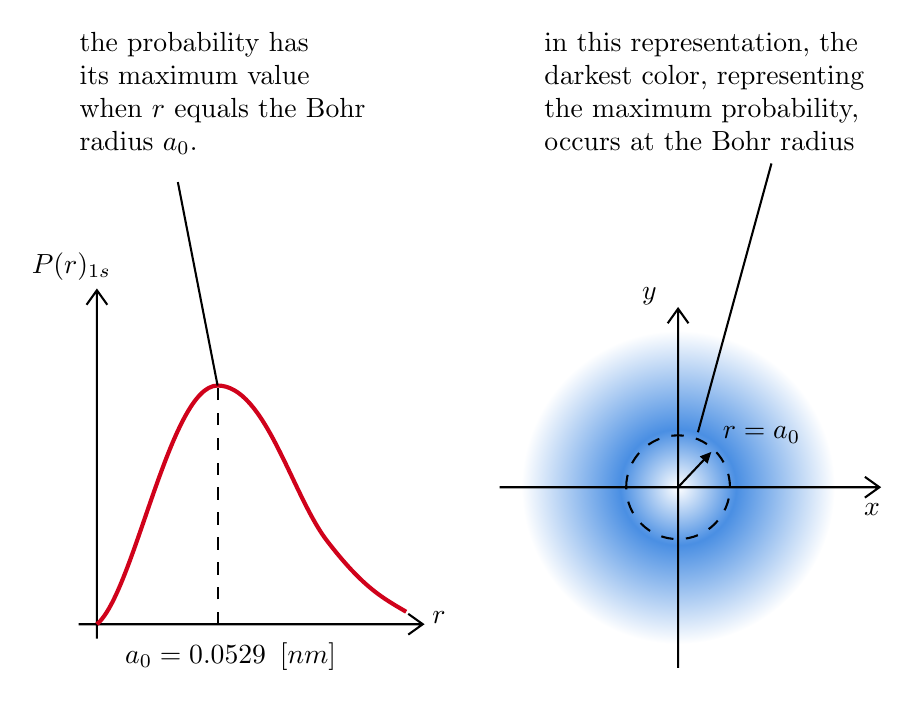
\begin{tikzpicture}[x=0.75pt,y=0.75pt,yscale=-1,xscale=1]
		%uncomment if require: \path (0,1129); %set diagram left start at 0, and has height of 1129
		
		%Shape: Circle [id:dp23040756811200813] 
		\draw  [draw opacity=0][shading=_09hu1pm1x,_f001ae7un][dash pattern={on 4.5pt off 4.5pt}] (368.36,286.91) .. controls (368.36,245.22) and (402.17,211.41) .. (443.86,211.41) .. controls (485.56,211.41) and (519.36,245.22) .. (519.36,286.91) .. controls (519.36,328.61) and (485.56,362.41) .. (443.86,362.41) .. controls (402.17,362.41) and (368.36,328.61) .. (368.36,286.91) -- cycle ;
		%Shape: Axis 2D [id:dp6575230635987284] 
		\draw  (155,352.91) -- (320.86,352.91)(163.86,192) -- (163.86,359.91) (313.86,347.91) -- (320.86,352.91) -- (313.86,357.91) (158.86,199) -- (163.86,192) -- (168.86,199)  ;
		%Straight Lines [id:da34848965342752236] 
		\draw  [dash pattern={on 4.5pt off 4.5pt}]  (222,353) -- (222,237.91) ;
		%Shape: Axis 2D [id:dp5970783323233091] 
		\draw  (357.86,286.91) -- (540.86,286.91)(443.86,200.91) -- (443.86,373.91) (533.86,281.91) -- (540.86,286.91) -- (533.86,291.91) (438.86,207.91) -- (443.86,200.91) -- (448.86,207.91)  ;
		%Curve Lines [id:da4887020200724457] 
		\draw [color={rgb, 255:red, 208; green, 2; blue, 27 }  ,draw opacity=1 ][line width=1.5]    (163.86,352.91) .. controls (181.86,337.91) and (199.14,237.91) .. (222,237.91) .. controls (244.86,237.91) and (257.86,290.91) .. (274.86,312.91) .. controls (291.86,334.91) and (300.86,339.91) .. (312.86,346.91) ;
		%Shape: Circle [id:dp546725505321543] 
		\draw  [dash pattern={on 4.5pt off 4.5pt}] (418.86,286.91) .. controls (418.86,273.11) and (430.06,261.91) .. (443.86,261.91) .. controls (457.67,261.91) and (468.86,273.11) .. (468.86,286.91) .. controls (468.86,300.72) and (457.67,311.91) .. (443.86,311.91) .. controls (430.06,311.91) and (418.86,300.72) .. (418.86,286.91) -- cycle ;
		%Straight Lines [id:da3051277137315207] 
		\draw    (443.86,286.91) -- (457.81,272.1) ;
		\draw [shift={(459.86,269.91)}, rotate = 133.26] [fill={rgb, 255:red, 0; green, 0; blue, 0 }  ][line width=0.08]  [draw opacity=0] (5.36,-2.57) -- (0,0) -- (5.36,2.57) -- cycle    ;
		%Straight Lines [id:da4383061946441076] 
		\draw    (202.86,139.91) -- (222,237.91) ;
		%Straight Lines [id:da3721801656262389] 
		\draw    (488.86,130.91) -- (453.43,260.41) ;
		
		% Text Node
		\draw (324,345.4) node [anchor=north west][inner sep=0.75pt]    {$r$};
		% Text Node
		\draw (131,172.4) node [anchor=north west][inner sep=0.75pt]    {$P(r)_{1s}$};
		% Text Node
		\draw (176,360.4) node [anchor=north west][inner sep=0.75pt]    {$a_{0} =0.0529\ \left[\text{nm}\right]$};
		% Text Node
		\draw (532,293.4) node [anchor=north west][inner sep=0.75pt]    {$x$};
		% Text Node
		\draw (425,189.4) node [anchor=north west][inner sep=0.75pt]    {$y$};
		% Text Node
		\draw (464,256.4) node [anchor=north west][inner sep=0.75pt]    {$r=a_{0}$};
		% Text Node
		\draw (154,66) node [anchor=north west][inner sep=0.75pt]   [align=left] {the probability has\\its maximum value\\when $\displaystyle r$ equals the Bohr\\radius $\displaystyle a_{0}$.};
		% Text Node
		\draw (378,66) node [anchor=north west][inner sep=0.75pt]   [align=left] {in this representation, the\\darkest color, representing\\the maximum probability,\\occurs at the Bohr radius};
		\end{tikzpicture}
		\vspace*{3mm}
		\caption[Probability of finding the electron as a function of distance from the nucleus for the hydrogen atom in the $1s$ state]{Probability of finding the electron as a function of distance from the nucleus for the\\ hydrogen atom in the $1s$ state (source: \cite{serway2018physics})}
	\end{figure}
	The peak of the curve corresponds to the most likely value of $r$ for this particular state. We prove easily that this peak occurs at the Bohr radius (just set the derivative of $P(r)_{1s}$ with respect to $r$ to zero), the radial position of the electron when the hydrogen atom is in its ground state in the Bohr theory, another agreement between the Bohr theory and the quantum theory!
	
	\paragraph{Potential Profile}\mbox{}\\\\\
	Let us come back on an important point that is often used in physics book but never proved (as far as we know): the quantum potential profile of the hydrogen-like atom. Many books sometimes speak of "\NewTerm{harmonic model of the atomic bonding}\index{harmonic model of the atomic bonding}" but it seems that this is a priori rather a misnomer.

	So we saw much earlier in this section that:
	
	In view of the interpretation of the three terms of the Hamiltonian, it is customary to say that the two terms:
	
	constitute the "\NewTerm{effective potential energy}\index{effective potential energy}\label{effective potential hydrogen atom}", thus explicitly:
	
	So the first term is (logically) repulsive while the second is attractive. A plot in Maple 4.00b of the effective potential energy gives with real experimental values for the radius with the real values of the constants:\\
	
	\texttt{>plot([-2.31E-28/r+6.11E-39*0*(0+1)/r\string^2,-2.31E-28/r+6.11E-39*1*(1+1)/r\string^2,\\-2.31E-28/r+6.11E-39*2*(2+1)/r\string^2,-2.31E-28/r+6.11E-39*3*(3+1)/r\string^2,\\-2.31E-28/r+6.11E-39*10*(10+1)/r\string^2],r=5E-11..10E-10,\\y=-0.5E-17..0.5E-17,thickness=2);}
	\begin{figure}[H]
		\begin{center}
		\includegraphics{img/chemistry/effective_potential_energy.jpg}
		\end{center}	
		\caption{Plot of the effective potential energy in Maple 4.00b for various $l$ and $Z$}
	\end{figure}
	where the legends were added afterwards with a text processor software. The reader will notice especially the case where $l=1$ that matches to the case of the figure indicated by the majority of graduate books of physics. Either with a zoom:\\

	\texttt{>plot(-2.31E-28/r+6.11E-39*1*(1+1)/r\string^2,r=5E-11..10E-10,thickness=2, color=green);}
	\begin{figure}[H]
		\begin{center}
		\includegraphics{img/chemistry/effective_potential_energy_l_equal_1.jpg}
		\end{center}	
		\caption{Plot of the famous effective potential energy in Maple 4.00b for  $l=1$ and $Z=1$}
	\end{figure}

	The first graph also tells us quite clearly that for $l= 0$ the electron has a negative potential energy that firmly holds it in the orbit of the proton. By cons already at $l= 1$ we guess that the point of stability of the electron is where the derivative is zero. Beyond the $l= 1$, in the case of a nucleus with a single proton, the electron is not naturally linked anymore since its potential energy tends to be positive. The reader can also have fun with Maple by making vary $Z$ and $l$. He will see that the effective potential energy is very sensitive to these parameters. For example, the plot below shows the effective potential energy with $l= 4$ and $Z = 1$ (thus unstable atom) and then with $l = 4$ and $Z = 6$ (which corresponds rather to an excited state):\\

	\texttt{>plot([-2.31E-28*1/r+6.11E-39*4*(4+1)/r\string^2,-2.31E-28*6/r+6.11E-39*4*(4+1)/r\string^2],\\r=5E-11..10E-10,thickness=2);}
	\begin{figure}[H]
		\begin{center}
		\includegraphics{img/chemistry/effective_potential_energy_l_equal_1_varous_z.jpg}
		\end{center}	
		\caption{Plot of the effective potential energy for $l=1$ and various $Z$}
	\end{figure}
	
	It is customary in practice to consider that:
	
	is to a given factor (electric charge factor) an "\NewTerm{effective electrical potential}\index{effective electrical potential}" or "\NewTerm{electric screened potential}\index{electric screened potential}". Indeed by defining the electric potential (\SeeChapter{see section Electrostatics page \pageref{electric potential}}), there are only an electric charge factor ratio between the electric potential energy and the electric potential. So we have:
	
	
	\begin{flushright}
	\begin{tabular}{l c}
	\circled{90} & \pbox{20cm}{\score{3}{5} \\ {\tiny 49 votes,  66.12\%}} 
	\end{tabular} 
	\end{flushright}

	%to make section start on odd page
	\newpage
	\thispagestyle{empty}
	\mbox{}
	\section{Molecular Chemistry}\label{molecular chemistry}
	\lettrine[lines=4]{\color{BrickRed}M}{olecular chemistry} is the central area that interconnects thanks to the study of molecules many promising advanced technologies of the early 121st century (holocene calendar) which are to name only the best known: molecular biology, molecular materials, molecular electronics, polymers, etc.
Orbital approximation

	Knowing it was found experimentally that a single molecule can have several very different functions, its theoretical study allows to use them better (sometimes better performance in terms of R\&D) in its areas of application. The reader will therefore understand that, as usually in this book, we will focus here only on the theoretical aspect (mathematical) of molecular chemistry even if we limit ourselves only to theoretical developments made between the years 11910 (holocene calendar) and about 11935 according to holocene calendar (beyond the complexity of the modern theories require too many pages to a general book like this one).
	
	We are in the beginning of the 121st century (holocene calendar) at the infancy of the discovery of what nature has done with plenty of time and chance (probabilities): that is to say complex molecules working as nano-machines capable locally (active site) to filter, oxidize, to make catalysis ... and many other manipulations (there is just to observe your own body!).
	
	A molecule is often treated in school classes with the Schrödinger equation (so no relativistic case and no consideration of the spins) in the usual form (\SeeChapter{see section Wave Quantum Physics page \pageref{schrödinger hamiltonian}}):
	
	or also in a stationary from (time-independent) where as a reminder $\Psi$ is a eigenfunctions and $E$ an eigenvalue of the application $H$.
	
	In reality, the wave functions are impossible to calculate normally with contemporary mathematical tools and the only thing we can do are numerical calculations (perturbation method). This is why some chemistry centers are transformed over time into data centers where the predictive character (and inexpensive) of quantum chemistry is becoming more and more important.
	
	It remains of course essential, as always, to understand how the theoretical models are built and their underlying assumptions.
	
	But we can still thanks to calculations predict the form of reasonable size of molecules, the energy of their internal connections, their energy capacity under stress deformation, the shape of the molecular orbitals (M.O.), energy state transitions (when parts of the molecule move therein), their reactivity vis-a-vis of a reaction medium...
	
	We commonly distinguish two cases of study of the molecular chemistry:
	\begin{enumerate}
		\item Quantum mechanics: all interactions between particles are taken into account under the assumption of some acceptable simplifications.
		\item Molecular mechanics: For large molecules, we are not concerned anymore over the electronic problem, but the interaction of certain parameters on which we want to focus.
	\end{enumerate}
	For example, haemoglobin (protein carrying oxygen carrying in the muscles) is a huge molecular structure which we will study only active site with the tools of quantum mechanics. The overall behaviour of the molecule itself is treated with the molecular mechanics tools.
	
	It follows that excepts for hydrogen-like atoms, we can not analytically describe a molecule from a purely quantum point of view! All current quantum methods rely on one or more approximations. The wave functions are therefore approximated and the level of calculation is adjusted according to what we want to show and the precision that we seek (seeking to minimize the computation time for cost problems...). The good understanding of approximations permits to express simple models requiring only a minimum of calculations (often trivial).
	
	We propose here to show two common models (and the most simplest):
	
	\subsection{Orbital Approximations}
	A molecule is obviously an extremely complex problem: $N$ nuclei, $n$ electrons and everything is moving!
	\begin{figure}[H]
		\begin{center}
		\includegraphics{img/chemistry/vibrating_molecule.jpg}
		\end{center}	
		\caption{Example of molecule where a almost everything is moving}
	\end{figure}
	The Hamiltonian (\SeeChapter{see section Wave Quantum Physics page \pageref{hamiltonian operator wave quantum physics}}):
	
	is then a nightmare but in the intuitive form (the subscript $G$ of the Hamiltonian means "General") below:
	
	where:
	
	\begin{enumerate}
		\item $\displaystyle-\sum_{k=1}^{N}\frac{\hbar^2}{2M_k}\vec{\nabla}_k^2$ is the kinetic energy of the $k$ nuclei of mass $M_k$ in the molecule.

		\item $\displaystyle-\sum_{i=1}^{n}\frac{\hbar^2}{2m_e}\vec{\nabla}_i^2$  is the kinetic energy of the $n$ electrons of mass $m_e$.

		\item $\displaystyle-\sum_{k=1}^{N}\sum_{i=1}^{n}\frac{Ze^2}{4\pi\varepsilon_0 r_{ik}}$ is the potential energy due to the attraction electron($-$)/nucleus($+$).

		\item $\displaystyle\mathop{\sum_{i=1}}_{j>1}^{n-1}\frac{e^2}{4\pi\varepsilon_0 r_{ik}}$ is the potential energy of the repulsion electron($-$)/electron($-$).

		\item $\displaystyle\mathop{\sum_{k=1}}_{i>k}^{N-1}\frac{Z_kZ_ie^2}{4\pi\varepsilon_0 r_{ik}}$ is the potential energy of repulsion nucleus($+$)/nucleus($+$).
	\end{enumerate}

	Often we find these terms in the following form of the Schrödinger equation in the literature:
	
	A first approximation we might try is to decouple the movement of the nuclei of the electrons. Indeed, as the nucleus is much more massive (about $2,000$ times) than the cloud of electrons, the center of mass is assimilated to the nucleus of the atom and all the motion to the entire electron cloud. This approximate approach is well known under the name "\NewTerm{Born-Oppenheimer approximation}\index{Born-Oppenheimer approximation}":
	
	which then allows us to study the molecular orbitals. But unfortunately this approximation is not sufficient because of the repulsion inter-electronic term (the double sum) that prevents using the separation of variables technique as we did in the section of Quantum Chemistry with the hydrogenoid-atom.
	
	Moreover, this latter equation is also written as the first line of the couple of equations below (Schrödinger equation of electrons and nuclei):
	\begin{subequations}
		\begin{align}
		&\underbrace{(T_e+V_{ee}+V_{en})}_{H_{\text{el}}}\Psi_{\text{el}}=E\Psi_{\text{el}}\\
		&\underbrace{(T_n+V_{nn})}_{H_{\text{nuclei}}}\Psi_n\Psi_{\text{el}}=E\Psi_n\Psi_{\text{el}}
		\end{align}
	\end{subequations}
	This system of equations is what some name the "\NewTerm{adiabatic approximation}\index{adiabatic approximation}" (???).
	
	The idea that then comes to mind will be using the following property:
	
	Given two operators $A$ and $B$, $f (u)$ and $g(v)$ their respective eigenfunctions associated with eigenvalues $a$ and $b$. Then $f (u) g (v)$ is an eigenfunction of the operator $A + B$ with associated eigenvalue $a + b$.

	Which is written:
	
			
	\begin{dem}
		We have:
		
		\begin{flushright}
			$\blacksquare$  Q.E.D.
		\end{flushright}
	\end{dem}
	And that's what we will use to break the $n$-electronic Hamiltonian $H_{\text{el}}$ into a sum of independent-electron Hamiltonian knowing of the above that if we find the eigenfunction for each (which is relatively easier) it will be sufficient to simply multiply them to get the overall eigenfunction!

	Thus, we write:
	
	and therefore we have to find for each $i$:
	
	Then we have:
	
	with therefore:
	
	This approach by one-electron Hamiltonian approach will lead us to replace:
	
	by the sum of Hamiltonian for an electron named "\NewTerm{effective Hamiltonian}\index{effective Hamiltonian}":
	
	This approximation method is sometimes named in theoretical chemistry "\NewTerm{independent electron approximation}\index{independent electron approximation}" or "\NewTerm{orbital approximation}\index{orbital approximation}". It consists therefore to include the electron-electron interactions and to write that each electron moves in an average potential resulting from the presence of all other electrons.
	
	The "\NewTerm{Slater method}\index{Slater method}" consists by definition to write the latter relation in the form:
	
	where $\sigma$ is named the "\NewTerm{screen constant}\index{screen constant}".
	
	The Slater method basically means replacing the purely electronic terms by a constant. It can be regarded as a parametric method since the constants were determined purely experimentally.
	
	The principle of empirical calculation of the screening constant is relatively simple: In a poly-electronic atom, the core electrons are on much contracted orbits  while the valence electrons that will be responsible for the chemical properties of the atom in question are on orbits much more "relaxed".
	
	The attraction of the nucleus on the latter electrons is much lower than that exerted on the core electrons and these electrons only receive a portion of the atomic charge.
	
	Slater then proposed that the effective charge, which is usually denoted by $Z^*$ could be calculated by taking into account the screening constant. This constant represents then the average effect of the other electrons on the considered electron  of the effective Hamiltonian $i$:
	
	For a peripheral electron, we will need to consider its screen constant is due to all electrons placed on orbits equal or below its own. The tradition (or rather the "trick") is that the calculation is done by combining atomic orbitals in several groups $1s/2s, 2p/3s, 3p/3d/4s, 4p/4d/4f/5s, 5p/$ etc.
	
	Then the calculation is simple because it is based on an array of predefined values and we simply have to add the screening contributions of all the electrons following the table below:
	\begin{table}[H]
		\centering
		\begin{tabular}{ccccc}\hline
		& $n'<n-1$ & $n'=n-1$ & $n'=n$ & $n'>n$ \\\hline
		1$s$ & & & $0.30$ & $0$ \\
		n$s$, n$p$ & $1$ & $0.85$ & $0.35$ & $0$ \\
		n$d$, n$f$ & $1$ & $1$ & $0.35$ & $0$\\ \hline
		\end{tabular}
		\caption{Screening contributions of electrons}
	\end{table}
	This table deserves some explanation of course !:
	
	The index indicates the number of the group that contributes to the screening constant while $n$ is the number of the group of electron that we consider.
	
	\pagebreak
	\begin{tcolorbox}[colframe=black,colback=white,sharp corners]
	\textbf{{\Large \ding{45}}Example:}\\\\
	In the case of the Carbon of configuration $1s^2 2s^2 2p^2$, the nuclear charge is $Z=6$. One electron $1s$ is shielded by only the another $1s$ electron, the effective charge it sees is therefore:
	
	A $2s$ or $2p$ electron is shielded by the two $1s$ electrons and by the other $3$ electrons $2s$ and $2p$. The effective charge by which it is attracted is then:
	
	So we see that the effective charge experienced decreases rather quickly!
	\end{tcolorbox}
	
	\subsection{LCAO Method}
	A linear combination of atomic orbitals or LCAO is a quantum superposition of atomic orbitals and a technique for calculating molecular orbitals in quantum chemistry. In quantum mechanics, electron configurations of atoms are described as wave functions. In mathematical sense, these wave functions are the basis set of functions, the basis functions, which describe the electrons of a given atom. In chemical reactions, orbital wave functions are modified, i.e. the electron cloud shape is changed, according to the type of atoms participating in the chemical bond.
	
	So as already mentioned, this method, rather qualitative, considers that the molecular wave function is a "\NewTerm{Linear Combination of Atomic Orbitals}\index{linear combination of atomic orbitals}" (LCAO) unlike the previous method where we multiply the effective Hamiltonian.
	
	This method is important because it is the basis of much of the current vocabulary of chemists when the chemistry done is cutting edge one!
	
	Let us take the example of the dihydrogen molecule $\mathrm{H}_2$. The idea is then following:
	
	If we have the function of the atomic orbital $1s_A$ of $\mathrm{H}_1$ and respectively the function $1s_B$ of $\mathrm{H}_B$, then we assume that the dicentric molecular orbital (linked to two atoms) thereof is given by:
	
	which defines a quantum system with two eigenstates.

	But as we well know, in reality, only the square of the wave function has a physical sense (probability of presence). Thus, if we assume that the wave function has no value in $\mathbb{C}$, we have for the single electron of interest ($1s$):
	
	where we assume that:
	\begin{itemize}
		\item $a^2\Psi_A^2$ represents the probability of presence to be near $A$.
		\item $b^2\Psi_B^2$ represents the probability of presence to be near $B$.
		\item $2ab\Psi_A\Psi_B$ represents the probability of presence of the electron that do the link $A-B$.
	\end{itemize}
	In the particular case of the symmetric diatomic molecule we have chosen as an example, the atoms $A$ and $B$ perform the same function and there is no reason that the electron is closer to $A$ than to $B$ or vice versa.

	Thus, the probability of finding the electron near $A$ is equal to the probability of finding it near $B$.
	
	Moreover, in this case the orbitals $\Psi_A$ and $\Psi_B$ are completely identical ($1s$ orbitals, both of the same atom) and there is therefore no need to distinguish them. So we have:
	
	We have two solutions for $\Psi_{AB}$ that are (these two solutions can be found in very different notations in the literature):
	
	and:
	 
	
	\begin{tcolorbox}[enhanced,colback=red!5!white,colframe=black!50!red,boxrule=1pt,arc=0pt,outer arc=0pt,drop lifted shadow,after skip=10pt plus 2pt]
	\bcbombe Caution! We can not put for the last two relations that $\Psi_A=\Psi_B$. The latter equality occurs at any point only if the distance between the two nucleus is zero (which is unlikely) or, if they are spaced a distant of a certain value $D$ in the middle thereof.
	\end{tcolorbox}
	
	These two expressions are simultaneously solutions of the Schrödinger equation. So we get two molecular orbitals from the two atomic orbitals in the case of symmetrical diatomic molecule.
	
	The function:
	
	is named "\NewTerm{bonding function}\index{bonding function}" because it corresponds to a reinforcement of the probability of presence of the electron between atoms $A$ and $B$ which corresponds to the creation of the bond!
	\begin{figure}[H]
		\begin{center}
		\includegraphics{img/chemistry/bonding_link.jpg}
		\end{center}	
	\end{figure}
		
	Conversely, the function:
	
	is named "\NewTerm{anti-bonding function}\index{anti-bonding function}" because it corresponds to a reduction of the probability of presence of the electron between atoms $A$ and $B$ which corresponds to the destruction of the bond!
	\begin{figure}[H]
		\begin{center}
		\includegraphics{img/chemistry/bonding_unlink.jpg}
		\end{center}	
	\end{figure}
	
	Ultimately, by overlapping, the two atomic orbitals with the same energy give birth to two molecular orbitals of different energy, a stabilized binding and the other anti-bonding destabilized.

	We have obviously from what we see just above that, in more complex cases, the energy level of the bonding molecular orbital is smaller than the anti-bonding (we will prove this rigorously in details below).

	Thus, it takes more energy to ionize respectively the electron of the binding orbital $\sigma$ than to ionize the electron of the anti-bonding orbital $\sigma^{*}$. It is commonly accepted that the energy of the bond function is stronger than the anti-bonding one (but we will make the proof further below).

	Let us also indicate that in chemistry, a chemical bond wherein each of the bonded atoms is sharing an electron from one of its outer layers to form a pair of electrons linking two atoms is commonly known as "\NewTerm{covalent bond}\index{covalent bond}".
	
	The chemists then say the covalent bond involves the equitable sharing of only one pair of electrons, named "\NewTerm{bonding pair}\index{bonding pair}" (but in fact where only one electron is really shared). Each atom provides an electron, the electron pair is then delocalized between two atoms as we have shown.

	These are the reasons why we commonly say that the bond $\sigma$ is a covalent chemical bond between two atoms created by orbital axial overlap.

	Now let us in-deep this approach! The molecular orbitals are to be normalized as we know. Which means that:
	
		What gives, since the atomic orbitals are normalized for $\Psi_1$ and are real functions:
	
	Since $a$ (real number in our case) is imposed as a constant, it comes immediately:
	
	Therefore for $\Psi_{AB}^1$:
	
	Identically, we have for $\Psi_{AB}^2$:
	
	If we have $S_{12}\ll 1$, it comes the following format that we find in many books:
	
	Let us make a small example using as orbital, the lowest atomic orbital (1$s$) of the hydrogen atom in the case of a dihydrogeneous bond $\mathrm{H}_2$ for which we have proved at the end of the section of Quantum Chemistry (see page \pageref{atomic orbitals of hydrogen atom}) that:
	
	Therefore it comes:
	
	with for recall:
	
	It comes then for the molecular binding orbital of level $s$:
	
	and for the anti-bonding of also the $s$ level:
	
	We then see immediately that $\sigma^*_s$ vanishes in the middle of the two protons because in this place $r_1=r_2$. The molecular anti-bonding orbital therefore has a nodal plane and the electrons are mainly located on the protons.
	
	By cons, for the molecular orbital $\sigma_s$ the density does not vanish. Then we understand easily that an electron of $\sigma_s$ ensures the stability of the molecule and is therefore responsible for the chemical bond.
	
	We therefore conclude that the electronic stabilization due to the two identical orbital interaction is proportional to their recovery. More the recovery is big, the more the stabilization is important.
	
	There is a more technical approach using Dirac notation (\SeeChapter{see section Wave Quantum Physics page \pageref{dirac formalism}}) and that has the advantage of allowing the determination of the eigenvalues of energy.

	First we write the general expression of the time independent Schrödinger equation with the Bra-Ket notation for one molecular orbital, superposition of two atomic orbitals:
	
	Either in explicit form:
	
	If we multiply by the bra $\langle \Psi_A|$  on the left and taking into account that $a$, $b$ and the specific eigenvalues of the energy are constants, we get the following equation:
	
	Similarly, we get the bra $\langle \Psi_B|$:
	
	Let us simplify the notations even more:
	
	By symmetry of the problem in the case of dihydrogen, we put:
	
	which are named "\NewTerm{resonance integrals}\index{resonance integrals}" because it is a term relating to the combination (resonance) of the both atomic orbital relative to the two atoms that made the molecular structure.

	We also have:
	
	which are named "\NewTerm{Coulomb integrals}\index{Coulomb integrals}" because they correspond according to the fifth postulate of Wave Quantum Physics (see section of the same name page \pageref{fifth postulate of wave quantum physics}) to the average value of the total energy of the electron.

	We have obviously:
	
	which are named "\NewTerm{recovery integrals}\index{recovery integrals}" because the two atomic orbitals of the same type of each atom overlap.
	
	And finally, we have always by symmetry of our particular case:
	
	We can then write, since the recovery integrals are unitary:
	
	These two equations are named "\NewTerm{secular equations}\index{secular equations}". The trivial solution is a priori not physical because it would mean that the electron has a zero probability density at any point in the space corresponding at $a=b=0$.

	There is a non-trivial solution and unique solution if and only if the following determinant (\SeeChapter{see section Linear Algebra page \pageref{determinant}}), known in molecular chemistry under the name "\NewTerm{secular determinant}\index{secular determinant}", is equal to zero:
	
	As we have by symmetry in our particular case:
	
	Therefore it comes:
	
	Hence:
	
	This gives us two solutions ($+$):
	
	and minus ($-$):
	
	Therefore we have:	
	
	But to be able to calculate the energy levels in detail, we must still have the shape of the Hamiltonian... and that using the both electrons of the dihydrogen molecule is quite difficult... To simplify the study, we reduce ourselves to the case of the cation (positive ion) $\mathrm{H}_2^{+}$ consisting of two protons and one electron:
	\begin{figure}[H]
		\centering
		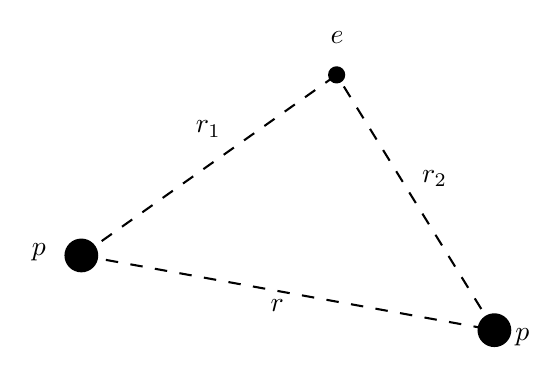
\begin{tikzpicture}[x=0.75pt,y=0.75pt,yscale=-1,xscale=1]
		%uncomment if require: \path (0,1129); %set diagram left start at 0, and has height of 1129
		
		%Shape: Circle [id:dp5499986525035587] 
		\draw  [fill={rgb, 255:red, 0; green, 0; blue, 0 }  ,fill opacity=1 ] (180.72,147.64) .. controls (180.72,143.42) and (184.14,140) .. (188.36,140) .. controls (192.58,140) and (196,143.42) .. (196,147.64) .. controls (196,151.86) and (192.58,155.28) .. (188.36,155.28) .. controls (184.14,155.28) and (180.72,151.86) .. (180.72,147.64) -- cycle ;
		%Shape: Circle [id:dp522960123376097] 
		\draw  [fill={rgb, 255:red, 0; green, 0; blue, 0 }  ,fill opacity=1 ] (379.72,183.64) .. controls (379.72,179.42) and (383.14,176) .. (387.36,176) .. controls (391.58,176) and (395,179.42) .. (395,183.64) .. controls (395,187.86) and (391.58,191.28) .. (387.36,191.28) .. controls (383.14,191.28) and (379.72,187.86) .. (379.72,183.64) -- cycle ;
		%Straight Lines [id:da6159552974618971] 
		\draw  [dash pattern={on 4.5pt off 4.5pt}]  (188.36,147.64) -- (387.36,183.64) ;
		%Shape: Circle [id:dp5696020161778541] 
		\draw  [fill={rgb, 255:red, 0; green, 0; blue, 0 }  ,fill opacity=1 ] (307.72,60.64) .. controls (307.72,58.63) and (309.35,57) .. (311.36,57) .. controls (313.37,57) and (315,58.63) .. (315,60.64) .. controls (315,62.65) and (313.37,64.28) .. (311.36,64.28) .. controls (309.35,64.28) and (307.72,62.65) .. (307.72,60.64) -- cycle ;
		%Straight Lines [id:da04681976577320435] 
		\draw  [dash pattern={on 4.5pt off 4.5pt}]  (188.36,147.64) -- (311.36,60.64) ;
		%Straight Lines [id:da7423893604064817] 
		\draw  [dash pattern={on 4.5pt off 4.5pt}]  (387.36,183.64) -- (311.36,60.64) ;
		
		% Text Node
		\draw (278,167.4) node [anchor=north west][inner sep=0.75pt]    {$r$};
		% Text Node
		\draw (242,81.4) node [anchor=north west][inner sep=0.75pt]    {$r_{1}$};
		% Text Node
		\draw (351,105.4) node [anchor=north west][inner sep=0.75pt]    {$r_{2}$};
		% Text Node
		\draw (163,140.4) node [anchor=north west][inner sep=0.75pt]    {$p$};
		% Text Node
		\draw (396,181.4) node [anchor=north west][inner sep=0.75pt]    {$p$};
		% Text Node
		\draw (307,38.4) node [anchor=north west][inner sep=0.75pt]    {$e$};
		\end{tikzpicture}	 
		\vspace*{3mm}
		\caption{Simplified study of the dihydrogen cation $\mathrm{H}_2^+$}
	\end{figure}
	We then have base on the relation we have obtained at the beginning of this section:
	
	The following relation:
	
	where the first two terms in the brackets are for recall associated with the potential energy of the electron and the last to the potential repulsion energy of proton (the first term on the right of the equality is the kinetic energy of the electron).

	Now let us try to sort the energy of these two molecular orbitals. For this, we write:
	
	Let us recall that for a system to be stable, the energies  $E_n$ must be negatives, this corresponding to the stable states (we need a supply of energy to take them out) and request from us because of the shape of $E_2$:
	
	Knowing this it comes:
	
	Therefore, we see that the notations are not consistent with the use in quantum physics because normally the index $1$ is reserved to the lowest energy. So we will write in the future:
	
	with the associated eigenfunctions  $\Psi_1$ and $\Psi_2$ and therefore:
	
	We can also noticed an important thing! This is that if we consider the atoms in isolated, the interaction terms cancel and we have:
	
	Therefore we have the qualitative difference between a single atom and a simple diatomic (ionized) system:
	
	This means that the energy of the lowest level of a diatomic ionized molecule is less than the energy of a single atom which is near $\alpha$. This observation confirms that the system is stabilized in energy compared to two isolated atoms, which seems consistent with the experimental determination of the existence of such molecules.
	
	Traditionally chemists represent the energy differences in the following form for our particular case:
	\begin{figure}[H]
		\centering
		\begin{tikzpicture}[x=0.75pt,y=0.75pt,yscale=-1,xscale=1]
		%uncomment if require: \path (0,1467); %set diagram left start at 0, and has height of 1467
		
		% Gradient Info
		  
		\tikzset {_nr81jvdxk/.code = {\pgfsetadditionalshadetransform{ \pgftransformshift{\pgfpoint{157.95 bp } { -193.05 bp }  }  \pgftransformscale{2.34 }  }}}
		\pgfdeclareradialshading{_7i55vojkf}{\pgfpoint{-72bp}{88bp}}{rgb(0bp)=(1,1,1);
		rgb(0bp)=(1,1,1);
		rgb(25bp)=(0,0,0);
		rgb(400bp)=(0,0,0)}
		\tikzset {_xjfnb3ruj/.code = {\pgfsetadditionalshadetransform{ \pgftransformshift{\pgfpoint{89.1 bp } { -108.9 bp }  }  \pgftransformscale{1.32 }  }}}
		\pgfdeclareradialshading{_qvo7z63if}{\pgfpoint{-72bp}{88bp}}{rgb(0bp)=(1,1,1);
		rgb(0bp)=(1,1,1);
		rgb(25bp)=(0.8,0.8,0.8);
		rgb(400bp)=(0.8,0.8,0.8)}
		\tikzset{_rqhigc1uu/.code = {\pgfsetadditionalshadetransform{\pgftransformshift{\pgfpoint{89.1 bp } { -108.9 bp }  }  \pgftransformscale{1.32 } }}}
		\pgfdeclareradialshading{_znuak8hxa} { \pgfpoint{-72bp} {88bp}} {color(0bp)=(transparent!0);
		color(0bp)=(transparent!0);
		color(25bp)=(transparent!62);
		color(400bp)=(transparent!62)} 
		\pgfdeclarefading{_j94kirr09}{\tikz \fill[shading=_znuak8hxa,_rqhigc1uu] (0,0) rectangle (50bp,50bp); }
		  
		\tikzset {_idfsl9wex/.code = {\pgfsetadditionalshadetransform{ \pgftransformshift{\pgfpoint{157.95 bp } { -193.05 bp }  }  \pgftransformscale{2.34 }  }}}
		\pgfdeclareradialshading{_9uts3yjm3}{\pgfpoint{-72bp}{88bp}}{rgb(0bp)=(1,1,1);
		rgb(0bp)=(1,1,1);
		rgb(25bp)=(0,0,0);
		rgb(400bp)=(0,0,0)}
		  
		\tikzset {_4xgowlhsq/.code = {\pgfsetadditionalshadetransform{ \pgftransformshift{\pgfpoint{157.95 bp } { -193.05 bp }  }  \pgftransformscale{2.34 }  }}}
		\pgfdeclareradialshading{_04plfa57u}{\pgfpoint{-72bp}{88bp}}{rgb(0bp)=(1,1,1);
		rgb(0bp)=(1,1,1);
		rgb(25bp)=(0,0,0);
		rgb(400bp)=(0,0,0)}
		
		
		%Straight Lines [id:da7900055369637282] 
		\draw    (111,403) -- (111,54) ;
		\draw [shift={(111,52)}, rotate = 90] [color={rgb, 255:red, 0; green, 0; blue, 0 }  ][line width=0.75]    (10.93,-4.9) .. controls (6.95,-2.3) and (3.31,-0.67) .. (0,0) .. controls (3.31,0.67) and (6.95,2.3) .. (10.93,4.9)   ;
		%Straight Lines [id:da3622129680793498] 
		\draw [color={rgb, 255:red, 155; green, 155; blue, 155 }  ,draw opacity=1 ]   (93,116) -- (187.5,116) ;
		%Straight Lines [id:da506170228521788] 
		\draw [color={rgb, 255:red, 155; green, 155; blue, 155 }  ,draw opacity=1 ]   (93,316) -- (150.5,316) -- (187.5,316) ;
		%Straight Lines [id:da030806998457588275] 
		\draw [line width=2.25]    (293.5,114) -- (366,114) ;
		%Straight Lines [id:da08007335888436384] 
		\draw [line width=2.25]    (293.5,318) -- (366,318) ;
		%Straight Lines [id:da12850158492219843] 
		\draw [line width=2.25]    (208.5,233) -- (243.5,233) ;
		%Straight Lines [id:da734550464847334] 
		\draw [line width=2.25]    (408.5,233) -- (443.5,233) ;
		%Straight Lines [id:da46590081928837224] 
		\draw  [dash pattern={on 4.5pt off 4.5pt}]  (293.5,114) -- (243.5,233) ;
		%Straight Lines [id:da22861206842151427] 
		\draw  [dash pattern={on 4.5pt off 4.5pt}]  (366,114) -- (408.5,233) ;
		%Straight Lines [id:da6487207902496939] 
		\draw  [dash pattern={on 4.5pt off 4.5pt}]  (243.5,233) -- (293.5,318) ;
		%Straight Lines [id:da7410083429441541] 
		\draw  [dash pattern={on 4.5pt off 4.5pt}]  (366,318) -- (408.5,233) ;
		%Shape: Circle [id:dp7436285364719002] 
		\path  [shading=_7i55vojkf,_nr81jvdxk] (406,114) .. controls (406,105.72) and (412.72,99) .. (421,99) .. controls (429.28,99) and (436,105.72) .. (436,114) .. controls (436,122.28) and (429.28,129) .. (421,129) .. controls (412.72,129) and (406,122.28) .. (406,114) -- cycle ; % for fading 
		 \draw   (406,114) .. controls (406,105.72) and (412.72,99) .. (421,99) .. controls (429.28,99) and (436,105.72) .. (436,114) .. controls (436,122.28) and (429.28,129) .. (421,129) .. controls (412.72,129) and (406,122.28) .. (406,114) -- cycle ; % for border 
		
		%Straight Lines [id:da642727355726699] 
		\draw [color={rgb, 255:red, 0; green, 0; blue, 0 }  ,draw opacity=1 ]   (436,114) -- (467.5,114) ;
		%Shape: Circle [id:dp39021282594109397] 
		\path  [shading=_qvo7z63if,_xjfnb3ruj,path fading= _j94kirr09 ,fading transform={xshift=2}] (467.5,114) .. controls (467.5,105.72) and (474.22,99) .. (482.5,99) .. controls (490.78,99) and (497.5,105.72) .. (497.5,114) .. controls (497.5,122.28) and (490.78,129) .. (482.5,129) .. controls (474.22,129) and (467.5,122.28) .. (467.5,114) -- cycle ; % for fading 
		 \draw   (467.5,114) .. controls (467.5,105.72) and (474.22,99) .. (482.5,99) .. controls (490.78,99) and (497.5,105.72) .. (497.5,114) .. controls (497.5,122.28) and (490.78,129) .. (482.5,129) .. controls (474.22,129) and (467.5,122.28) .. (467.5,114) -- cycle ; % for border 
		
		%Shape: Circle [id:dp4911044129267639] 
		\path  [shading=_9uts3yjm3,_idfsl9wex] (406,302) .. controls (406,293.72) and (412.72,287) .. (421,287) .. controls (429.28,287) and (436,293.72) .. (436,302) .. controls (436,310.28) and (429.28,317) .. (421,317) .. controls (412.72,317) and (406,310.28) .. (406,302) -- cycle ; % for fading 
		 \draw   (406,302) .. controls (406,293.72) and (412.72,287) .. (421,287) .. controls (429.28,287) and (436,293.72) .. (436,302) .. controls (436,310.28) and (429.28,317) .. (421,317) .. controls (412.72,317) and (406,310.28) .. (406,302) -- cycle ; % for border 
		
		%Straight Lines [id:da02684615513951938] 
		\draw [color={rgb, 255:red, 0; green, 0; blue, 0 }  ,draw opacity=1 ]   (436,302) -- (467.5,302) ;
		%Shape: Circle [id:dp6208588497828584] 
		\path  [shading=_04plfa57u,_4xgowlhsq] (467.5,302) .. controls (467.5,293.72) and (474.22,287) .. (482.5,287) .. controls (490.78,287) and (497.5,293.72) .. (497.5,302) .. controls (497.5,310.28) and (490.78,317) .. (482.5,317) .. controls (474.22,317) and (467.5,310.28) .. (467.5,302) -- cycle ; % for fading 
		 \draw   (467.5,302) .. controls (467.5,293.72) and (474.22,287) .. (482.5,287) .. controls (490.78,287) and (497.5,293.72) .. (497.5,302) .. controls (497.5,310.28) and (490.78,317) .. (482.5,317) .. controls (474.22,317) and (467.5,310.28) .. (467.5,302) -- cycle ; % for border 
		
		
		% Text Node
		\draw (83,60.4) node [anchor=north west][inner sep=0.75pt]    {$E$};
		% Text Node
		\draw (119,33.4) node [anchor=north west][inner sep=0.75pt]    {$E\rightarrow 0$};
		% Text Node
		\draw (194.5,93.4) node [anchor=north west][inner sep=0.75pt]    {$E_{2} =\dfrac{\alpha -\beta }{1-S}$};
		% Text Node
		\draw (194,295.4) node [anchor=north west][inner sep=0.75pt]    {$E_{1} =\dfrac{\alpha +\beta }{1+S}$};
		% Text Node
		\draw (117,383.4) node [anchor=north west][inner sep=0.75pt]    {$E\rightarrow -\infty $};
		% Text Node
		\draw (192,228.9) node [anchor=north west][inner sep=0.75pt]    {$\alpha $};
		% Text Node
		\draw (212,214.4) node [anchor=north west][inner sep=0.75pt]    {$\Psi _{A}$};
		% Text Node
		\draw (409,214.4) node [anchor=north west][inner sep=0.75pt]    {$\Psi _{B}$};
		% Text Node
		\draw (448,227.9) node [anchor=north west][inner sep=0.75pt]    {$\alpha $};
		% Text Node
		\draw (287,221.4) node [anchor=north west][inner sep=0.75pt]    {$E_{1} < E_{2} < 0$};
		% Text Node
		\draw (504.5,106.4) node [anchor=north west][inner sep=0.75pt]    {$\Psi _{2}$};
		% Text Node
		\draw (504.5,293.4) node [anchor=north west][inner sep=0.75pt]    {$\Psi _{1}$};
		
		\end{tikzpicture}
		\vspace*{3mm}
		\caption{Energy levels of dihydrogen cation $\mathrm{H}_2$}
	\end{figure}
	We therefore conclude - by generalizing a little bit... - that when two atoms (each contributing with an electron) combine, their atomic orbitals will combine to generate two molecular orbitals, one of energy level $\Psi_1$ and the second of higher energy level $\Psi_2$ than that of the isolated atoms. Thus, the split up that will make leave one of the electron with one of atoms will be exothermic in comparison to the single atoms.
	
	Up to now we have discussed the electronic states of rigid molecules, where the nuclei are clamped to a fixed position. In this section we will improve our model of molecules and include the rotation and vibration of diatomic molecules.

	\pagebreak
	\subsection{Molecular Rotational Energy Levels}\label{molecular rotational energy levels}
	As we have seen in the section of Quantum chemistry, for analytical reasons we consider molecules as rigid rotators.

	The rigid rotators are commonly classified into four types:
	\begin{itemize}
		\item Spherical rotors: have equal moments of inertia (e.g., $\mathrm{CH}_4$).
		\begin{figure}[H]
			\centering
			\includegraphics{img/chemistry/molecule_ch4.jpg}
		\end{figure}
		
		\item Symmetric rotors: have two equal moments of inertial (e.g., $\mathrm{NH}_3$).
		\begin{figure}[H]
			\centering
			\includegraphics{img/chemistry/molecule_nh3.jpg}
		\end{figure}
		
		\item Linear rotors: have one moment of inertia equal to zero (e.g., $\mathrm{CO_2}$, $\mathrm{HCl}$).
		\begin{figure}[H]
			\centering
			\includegraphics{img/chemistry/molecule_co2.jpg}
		\end{figure}
		\begin{figure}[H]
			\centering
			\includegraphics{img/chemistry/molecule_hcl.jpg}
		\end{figure}

		\item Asymmetric rotors: have three different moments of inertia (e.g., $\mathrm{H}_2\mathrm{O}$).
		\begin{figure}[H]
			\centering
			\includegraphics{img/chemistry/molecule_h2o.jpg}
		\end{figure}
	\end{itemize}
	Let us now recall that we have proved in the section of Quantum Chemistry that for the rigid rotator (see page \pageref{quantum chemistry rigid rotator}) the part of the Hamiltonian dedicated to the rotation of energy is:
	
	Where $L^2$ was is an operator but from which we know from our study of Wave Quantum Physics (see page \pageref{eigenvalue of angular momentum}) that the eigenvalues are:
	
	and where $r$ is the distance between the two corpuscles (nucleus and electron in the context of our study of the hydrogenous atom in the section of Quantum Chemistry) and:
	
	In the context of diatomic molecules $A$ and $B$ it is more common to write $r_{AB}$ and:
	
	In the section of Wave Quantum Physics we have seen (page \pageref{angular momentum and spin}) that if we must consider the spin we have to write the more general form:
	
	with $J=0,1/2/,1,3/2,2,5/2,\ldots$. Therefore:
	
	In the old style spectroscopic literature, the rotational term values $F(J) = E(J)/hc$ are used instead of the energies....The previous relation is then written:
	
	with the "\NewTerm{rotational constant}\index{rotational constant}":
	
	We also know from the section of Classical Mechanics (page \pageref{moment of inertia}) that:
	
	Therefore:
	
	That simplifies to:
	
	Hence:
	
	
	The energy separation between the rotational levels $J$ and $J+1$ is given obviously by:
	
	and increase linearly with $J$.
	
	Let us now calculate the moment of inertia, that we will denoted $I$ to avoid the confusion with the orbital kinetic momentum $J$ used above, of a diatomic molecule. Let us imagine the diatomic molecule as a system of two tiny spheres at either end of a thin weightless rod.
	\begin{figure}[H]
		\centering
		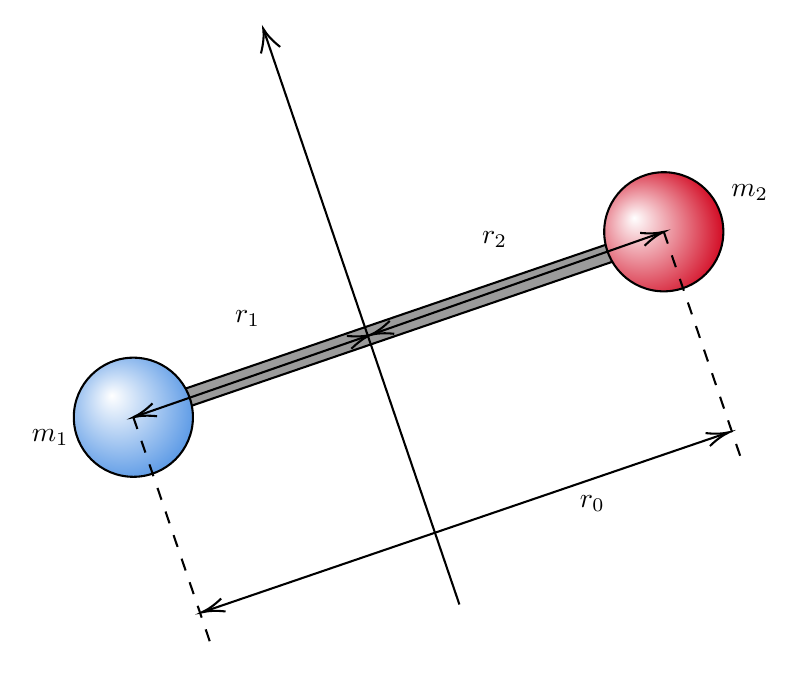
\begin{tikzpicture}[x=0.75pt,y=0.75pt,yscale=-1,xscale=1]
		%uncomment if require: \path (0,1046); %set diagram left start at 0, and has height of 1046
		
		% Gradient Info
		  
		\tikzset {_gchbgnjt2/.code = {\pgfsetadditionalshadetransform{ \pgftransformshift{\pgfpoint{85.8 bp } { -106.92 bp }  }  \pgftransformscale{1.32 }  }}}
		\pgfdeclareradialshading{_2wiaipo68}{\pgfpoint{-72bp}{88bp}}{rgb(0bp)=(1,1,1);
		rgb(0bp)=(1,1,1);
		rgb(25bp)=(0.29,0.56,0.89);
		rgb(400bp)=(0.29,0.56,0.89)}
		
		% Gradient Info
		  
		\tikzset {_9983br7fa/.code = {\pgfsetadditionalshadetransform{ \pgftransformshift{\pgfpoint{82.5 bp } { -110.22 bp }  }  \pgftransformscale{1.32 }  }}}
		\pgfdeclareradialshading{_4oje0xucs}{\pgfpoint{-72bp}{88bp}}{rgb(0bp)=(1,1,1);
		rgb(0bp)=(1,1,1);
		rgb(25bp)=(0.82,0.01,0.11);
		rgb(400bp)=(0.82,0.01,0.11)}
		
		%Shape: Rectangle [id:dp7207588054422036] 
		\draw  [fill={rgb, 255:red, 155; green, 155; blue, 155 }  ,fill opacity=1 ] (184.42,218.19) -- (458.13,124.54) -- (460.97,132.84) -- (187.26,226.49) -- cycle ;
		%Straight Lines [id:da5259317187341161] 
		\draw    (365.5,305.4) -- (271.64,29.89) ;
		\draw [shift={(271,28)}, rotate = 71.19] [color={rgb, 255:red, 0; green, 0; blue, 0 }  ][line width=0.75]    (10.93,-4.9) .. controls (6.95,-2.3) and (3.31,-0.67) .. (0,0) .. controls (3.31,0.67) and (6.95,2.3) .. (10.93,4.9)   ;
		%Shape: Circle [id:dp277756829912299] 
		\path  [shading=_2wiaipo68,_gchbgnjt2] (179.72,215.19) .. controls (179.72,199.34) and (192.57,186.49) .. (208.42,186.49) .. controls (224.27,186.49) and (237.12,199.34) .. (237.12,215.19) .. controls (237.12,231.04) and (224.27,243.89) .. (208.42,243.89) .. controls (192.57,243.89) and (179.72,231.04) .. (179.72,215.19) -- cycle ; % for fading 
		 \draw   (179.72,215.19) .. controls (179.72,199.34) and (192.57,186.49) .. (208.42,186.49) .. controls (224.27,186.49) and (237.12,199.34) .. (237.12,215.19) .. controls (237.12,231.04) and (224.27,243.89) .. (208.42,243.89) .. controls (192.57,243.89) and (179.72,231.04) .. (179.72,215.19) -- cycle ; % for border 
		
		%Shape: Circle [id:dp3127293846186161] 
		\path  [shading=_4oje0xucs,_9983br7fa] (435.27,125.84) .. controls (435.27,109.99) and (448.12,97.14) .. (463.97,97.14) .. controls (479.82,97.14) and (492.67,109.99) .. (492.67,125.84) .. controls (492.67,141.69) and (479.82,154.54) .. (463.97,154.54) .. controls (448.12,154.54) and (435.27,141.69) .. (435.27,125.84) -- cycle ; % for fading 
		 \draw   (435.27,125.84) .. controls (435.27,109.99) and (448.12,97.14) .. (463.97,97.14) .. controls (479.82,97.14) and (492.67,109.99) .. (492.67,125.84) .. controls (492.67,141.69) and (479.82,154.54) .. (463.97,154.54) .. controls (448.12,154.54) and (435.27,141.69) .. (435.27,125.84) -- cycle ; % for border 
		
		%Straight Lines [id:da18611233833816754] 
		\draw    (210.31,214.54) -- (320.81,176.17) ;
		\draw [shift={(322.7,175.51)}, rotate = 160.85] [color={rgb, 255:red, 0; green, 0; blue, 0 }  ][line width=0.75]    (10.93,-3.29) .. controls (6.95,-1.4) and (3.31,-0.3) .. (0,0) .. controls (3.31,0.3) and (6.95,1.4) .. (10.93,3.29)   ;
		\draw [shift={(208.42,215.19)}, rotate = 340.85] [color={rgb, 255:red, 0; green, 0; blue, 0 }  ][line width=0.75]    (10.93,-3.29) .. controls (6.95,-1.4) and (3.31,-0.3) .. (0,0) .. controls (3.31,0.3) and (6.95,1.4) .. (10.93,3.29)   ;
		%Straight Lines [id:da4734711783972716] 
		\draw    (324.58,174.85) -- (462.08,126.5) ;
		\draw [shift={(463.97,125.84)}, rotate = 160.63] [color={rgb, 255:red, 0; green, 0; blue, 0 }  ][line width=0.75]    (10.93,-3.29) .. controls (6.95,-1.4) and (3.31,-0.3) .. (0,0) .. controls (3.31,0.3) and (6.95,1.4) .. (10.93,3.29)   ;
		\draw [shift={(322.7,175.51)}, rotate = 340.63] [color={rgb, 255:red, 0; green, 0; blue, 0 }  ][line width=0.75]    (10.93,-3.29) .. controls (6.95,-1.4) and (3.31,-0.3) .. (0,0) .. controls (3.31,0.3) and (6.95,1.4) .. (10.93,3.29)   ;
		%Straight Lines [id:da1936064958327106] 
		\draw  [dash pattern={on 4.5pt off 4.5pt}]  (208.42,215.19) -- (246.23,326.08) ;
		%Straight Lines [id:da37343250823852836] 
		\draw  [dash pattern={on 4.5pt off 4.5pt}]  (463.97,125.84) -- (501.77,236.72) ;
		%Straight Lines [id:da6777110573636353] 
		\draw    (243.32,308.55) -- (493.61,223.05) ;
		\draw [shift={(495.5,222.4)}, rotate = 161.14] [color={rgb, 255:red, 0; green, 0; blue, 0 }  ][line width=0.75]    (10.93,-3.29) .. controls (6.95,-1.4) and (3.31,-0.3) .. (0,0) .. controls (3.31,0.3) and (6.95,1.4) .. (10.93,3.29)   ;
		\draw [shift={(241.42,309.19)}, rotate = 341.14] [color={rgb, 255:red, 0; green, 0; blue, 0 }  ][line width=0.75]    (10.93,-3.29) .. controls (6.95,-1.4) and (3.31,-0.3) .. (0,0) .. controls (3.31,0.3) and (6.95,1.4) .. (10.93,3.29)   ;
		
		% Text Node
		\draw (256,162.4) node [anchor=north west][inner sep=0.75pt]    {$r_{1}$};
		% Text Node
		\draw (375,124.4) node [anchor=north west][inner sep=0.75pt]    {$r_{2}$};
		% Text Node
		\draw (158,219.4) node [anchor=north west][inner sep=0.75pt]    {$m_{1}$};
		% Text Node
		\draw (495,101.4) node [anchor=north west][inner sep=0.75pt]    {$m_{2}$};
		% Text Node
		\draw (422,251.4) node [anchor=north west][inner sep=0.75pt]    {$r_{0}$};
		
		\end{tikzpicture} 
		\vspace*{3mm}	
		\caption{Construction for the study of inertia momentum of a diatomic molecule}
	\end{figure}
	Let $C$ be the center of mass of the molecule. Let $r_1$ and $r_2$ be the distances of the two atoms of respective masses $m_1$, $m_2$ from the center of mass $C$ of the molecule:
	We see that:
	
	and we have (\SeeChapter{see section Classical Mechanics page \pageref{center of mass}}):
	
	Therefore:
	
	Hence:
	
	After rearranging we get:
	
	or:
	
	Similarly:
	
	Let $I$ (instead of the traditional notation $J$) be the total moment of inertia of the diatomic molecule about an axis passing through the center of mass of the molecule and perpendicular to the bond length.

	Then we have seen in the section of Classical Mechanics (see page \pageref{moment of inertia}) that:
	
	or:
	
	thus:
	
	after simplification:
	
	Hence:
	
	So finally for a diatomic molecule (or any pair of object turning around a common center) we get the following moment of inertia\index{moment of inertia of a diatomic molecule}:
	
	Hence the fact that we often found in the literature the previous main relations under the form:
	
	and:
	
	\begin{figure}[H]
		\centering
		% Gradient Info
  
		\tikzset {_z826ptwnh/.code = {\pgfsetadditionalshadetransform{ \pgftransformshift{\pgfpoint{0 bp } { 0 bp }  }  \pgftransformrotate{-270 }  \pgftransformscale{2 }  }}}
		\pgfdeclarehorizontalshading{_n5iujtmp8}{150bp}{rgb(0bp)=(1,1,1);
		rgb(37.5bp)=(1,1,1);
		rgb(62.5bp)=(0.92,0.31,0.02);
		rgb(100bp)=(0.92,0.31,0.02)}
		\tikzset{every picture/.style={line width=0.75pt}} %set default line width to 0.75pt        
		
		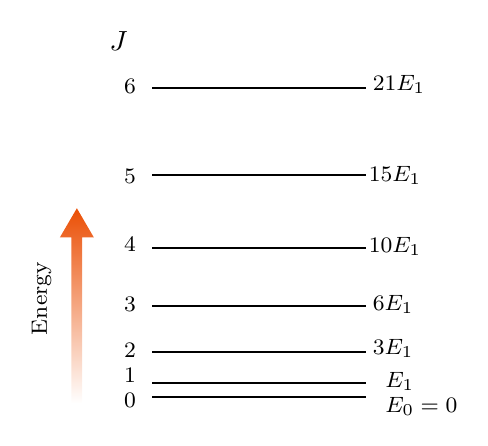
\begin{tikzpicture}[x=0.75pt,y=0.75pt,yscale=-1,xscale=1]
		%uncomment if require: \path (0,1129); %set diagram left start at 0, and has height of 1129
		
		%Straight Lines [id:da492243358004846] 
		\draw    (297,243) -- (399.86,243) ;
		%Straight Lines [id:da2321453668531881] 
		\draw    (297,236) -- (399.86,236) ;
		%Straight Lines [id:da7504183280008327] 
		\draw    (297,221) -- (399.86,221) ;
		%Straight Lines [id:da9917877117882574] 
		\draw    (297,199) -- (399.86,199) ;
		%Straight Lines [id:da9773897554233759] 
		\draw    (297,171) -- (399.86,171) ;
		%Straight Lines [id:da7448145605612597] 
		\draw    (297,136) -- (399.86,136) ;
		%Straight Lines [id:da8139697214227404] 
		\draw    (297,94) -- (399.86,94) ;
		%Up Arrow [id:dp7276804673687078] 
		\draw  [draw opacity=0][shading=_n5iujtmp8,_z826ptwnh] (252.53,165.91) -- (260.7,151.91) -- (268.86,165.91) -- (263.28,165.91) -- (263.28,245.91) -- (258.11,245.91) -- (258.11,165.91) -- cycle ;
		
		% Text Node
		\draw (275,65.4) node [anchor=north west][inner sep=0.75pt]    {$J$};
		% Text Node
		\draw (282,239.4) node [anchor=north west][inner sep=0.75pt]  [font=\footnotesize]  {$0$};
		% Text Node
		\draw (282,227.4) node [anchor=north west][inner sep=0.75pt]  [font=\footnotesize]  {$1$};
		% Text Node
		\draw (282,215.4) node [anchor=north west][inner sep=0.75pt]  [font=\footnotesize]  {$2$};
		% Text Node
		\draw (282,193.4) node [anchor=north west][inner sep=0.75pt]  [font=\footnotesize]  {$3$};
		% Text Node
		\draw (282,164.4) node [anchor=north west][inner sep=0.75pt]  [font=\footnotesize]  {$4$};
		% Text Node
		\draw (282,131.4) node [anchor=north west][inner sep=0.75pt]  [font=\footnotesize]  {$5$};
		% Text Node
		\draw (282,88.4) node [anchor=north west][inner sep=0.75pt]  [font=\footnotesize]  {$6$};
		% Text Node
		\draw (237.5,214.5) node [anchor=north west][inner sep=0.75pt]  [rotate=-270] [align=left] {{\footnotesize Energy}};
		% Text Node
		\draw (407.86,241.4) node [anchor=north west][inner sep=0.75pt]  [font=\footnotesize]  {$E_{0} =0$};
		% Text Node
		\draw (407.86,229.4) node [anchor=north west][inner sep=0.75pt]  [font=\footnotesize]  {$E_{1}$};
		% Text Node
		\draw (401.86,213.4) node [anchor=north west][inner sep=0.75pt]  [font=\footnotesize]  {$3E_{1}$};
		% Text Node
		\draw (401.86,192.4) node [anchor=north west][inner sep=0.75pt]  [font=\footnotesize]  {$6E_{1}$};
		% Text Node
		\draw (399.86,164.4) node [anchor=north west][inner sep=0.75pt]  [font=\footnotesize]  {$10E_{1}$};
		% Text Node
		\draw (399.86,130.4) node [anchor=north west][inner sep=0.75pt]  [font=\footnotesize]  {$15E_{1}$};
		% Text Node
		\draw (401.86,86.4) node [anchor=north west][inner sep=0.75pt]  [font=\footnotesize]  {$21E_{1}$};
		\end{tikzpicture}
	\end{figure}
	Therefore, as: 
	
	the frequencies at which transitions can occur are given by :
	
	Notice that for $J_z=0$ we have a non-null zero point energy and frequency:
	
	
	\begin{tcolorbox}[colframe=black,colback=white,sharp corners]
	\textbf{{\Large \ding{45}}Example:}\\\\
	The molecule $\mathrm{NaH}$ is found to undergo a rotational transition from  $J=0$ to $J=1$ when it absorbs a photon of frequency $2.94 \cdot 10^{11}$ [Hz]. We want to know the equilibrium bond length of the molecule.\\

	For this purpose we use $J_z=0$ in the formula for the transition frequency:
	
	Solving for $r_0$ gives:
	
	The reduced mass is given by:
	
	which is in atomic mass units or relative units. In order to convert to kilograms, we need the conversion factor $1\;[\text{au}]= 1.66\cdot 10^{-27}$ [kg]. Multiplying this by $0.9655$ gives a reduced mass of $1.603\cdot 10^{-27}$ [kg]. Substituting in for $r_0$ gives:
	
	\end{tcolorbox}

	\pagebreak
	\subsection{Molecular Vibrational Energy Levels}\label{molecular vibrations}
	Let us consider the simple case of a vibrating diatomic molecule, where restoring force is proportional to displacement such that (\SeeChapter{see section Mechanics page \pageref{spring tension}}):
	
	The potential energy is as we have proved it in the previously mentioned section, but with the notation of Quantum Physics, given by:
	
	Now remember that we have proved in the section of Wave Quantum Physics (see page \pageref{schrodinger wave equation}), that the Schrödinger equation was given by:
	
	After rearrangement:
	
	And using the conventional notations in chemistry and quantum physics:
	
	Before continuing we need to study a bit this important configuration of masses:
	\begin{figure}[H]
		\centering		
		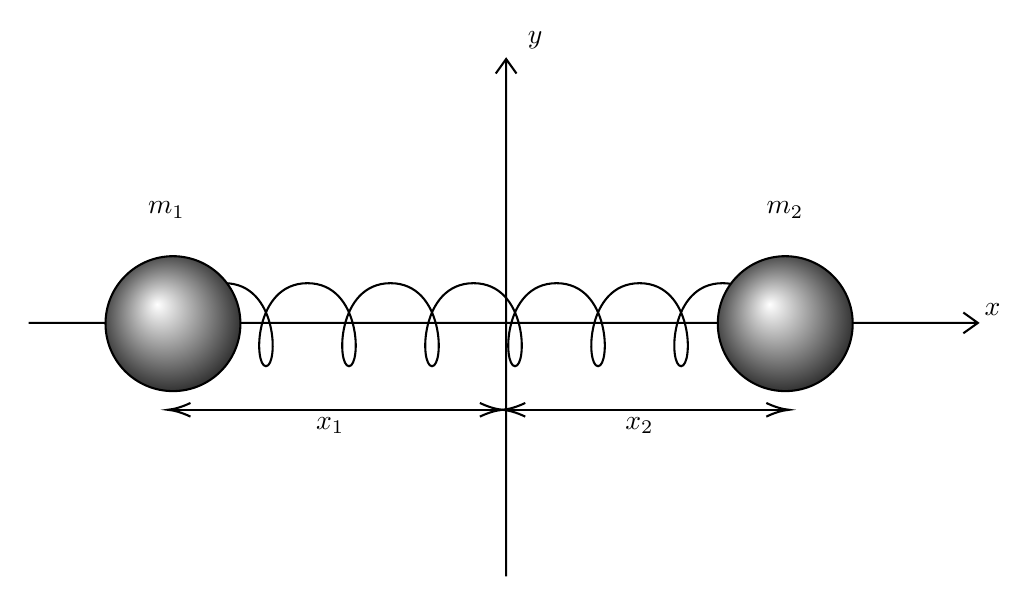
\begin{tikzpicture}[x=0.75pt,y=0.75pt,yscale=-1,xscale=1]
		%uncomment if require: \path (0,592); %set diagram left start at 0, and has height of 592
		
		% Gradient Info
		  
		\tikzset {_oxbdbhyt9/.code = {\pgfsetadditionalshadetransform{ \pgftransformshift{\pgfpoint{89.1 bp } { -108.9 bp }  }  \pgftransformscale{1.32 }  }}}
		\pgfdeclareradialshading{_g64p4pfml}{\pgfpoint{-72bp}{88bp}}{rgb(0bp)=(1,1,1);
		rgb(0bp)=(1,1,1);
		rgb(25bp)=(0,0,0);
		rgb(400bp)=(0,0,0)}
		
		% Gradient Info
		  
		\tikzset {_ejjdkk3ed/.code = {\pgfsetadditionalshadetransform{ \pgftransformshift{\pgfpoint{89.1 bp } { -108.9 bp }  }  \pgftransformscale{1.32 }  }}}
		\pgfdeclareradialshading{_k7jup6jxz}{\pgfpoint{-72bp}{88bp}}{rgb(0bp)=(1,1,1);
		rgb(0bp)=(1,1,1);
		rgb(25bp)=(0,0,0);
		rgb(400bp)=(0,0,0)}
		
		%Shape: Spring [id:dp4375106912641964] 
		\draw   (183.3,147) .. controls (209.3,147) and (209.3,187) .. (203.3,187) .. controls (197.3,187) and (197.3,147) .. (223.3,147) .. controls (249.3,147) and (249.3,187) .. (243.3,187) .. controls (237.3,187) and (237.3,147) .. (263.3,147) .. controls (289.3,147) and (289.3,187) .. (283.3,187) .. controls (277.3,187) and (277.3,147) .. (303.3,147) .. controls (329.3,147) and (329.3,187) .. (323.3,187) .. controls (317.3,187) and (317.3,147) .. (343.3,147) .. controls (369.3,147) and (369.3,187) .. (363.3,187) .. controls (357.3,187) and (357.3,147) .. (383.3,147) .. controls (409.3,147) and (409.3,187) .. (403.3,187) .. controls (397.3,187) and (397.3,147) .. (423.3,147) .. controls (424.71,147) and (426.04,147.12) .. (427.3,147.34) ;
		%Shape: Axis 2D [id:dp7767476921050476] 
		\draw  (89,166.14) -- (546.3,166.14)(319.02,39) -- (319.02,288.3) (539.3,161.14) -- (546.3,166.14) -- (539.3,171.14) (314.02,46) -- (319.02,39) -- (324.02,46)  ;
		%Shape: Circle [id:dp3936167598285336] 
		\path  [shading=_g64p4pfml,_oxbdbhyt9] (126,166.5) .. controls (126,148.55) and (140.55,134) .. (158.5,134) .. controls (176.45,134) and (191,148.55) .. (191,166.5) .. controls (191,184.45) and (176.45,199) .. (158.5,199) .. controls (140.55,199) and (126,184.45) .. (126,166.5) -- cycle ; % for fading 
		 \draw   (126,166.5) .. controls (126,148.55) and (140.55,134) .. (158.5,134) .. controls (176.45,134) and (191,148.55) .. (191,166.5) .. controls (191,184.45) and (176.45,199) .. (158.5,199) .. controls (140.55,199) and (126,184.45) .. (126,166.5) -- cycle ; % for border 
		
		%Shape: Circle [id:dp14545450490748557] 
		\path  [shading=_k7jup6jxz,_ejjdkk3ed] (421,166.5) .. controls (421,148.55) and (435.55,134) .. (453.5,134) .. controls (471.45,134) and (486,148.55) .. (486,166.5) .. controls (486,184.45) and (471.45,199) .. (453.5,199) .. controls (435.55,199) and (421,184.45) .. (421,166.5) -- cycle ; % for fading 
		 \draw   (421,166.5) .. controls (421,148.55) and (435.55,134) .. (453.5,134) .. controls (471.45,134) and (486,148.55) .. (486,166.5) .. controls (486,184.45) and (471.45,199) .. (453.5,199) .. controls (435.55,199) and (421,184.45) .. (421,166.5) -- cycle ; % for border 
		
		%Straight Lines [id:da22846869885087306] 
		\draw    (158,208) -- (315.3,208) ;
		\draw [shift={(317.3,208)}, rotate = 180] [color={rgb, 255:red, 0; green, 0; blue, 0 }  ][line width=0.75]    (10.93,-3.29) .. controls (6.95,-1.4) and (3.31,-0.3) .. (0,0) .. controls (3.31,0.3) and (6.95,1.4) .. (10.93,3.29)   ;
		\draw [shift={(156,208)}, rotate = 0] [color={rgb, 255:red, 0; green, 0; blue, 0 }  ][line width=0.75]    (10.93,-3.29) .. controls (6.95,-1.4) and (3.31,-0.3) .. (0,0) .. controls (3.31,0.3) and (6.95,1.4) .. (10.93,3.29)   ;
		%Straight Lines [id:da836310646813663] 
		\draw    (319.3,208) -- (453.3,208) ;
		\draw [shift={(455.3,208)}, rotate = 180] [color={rgb, 255:red, 0; green, 0; blue, 0 }  ][line width=0.75]    (10.93,-3.29) .. controls (6.95,-1.4) and (3.31,-0.3) .. (0,0) .. controls (3.31,0.3) and (6.95,1.4) .. (10.93,3.29)   ;
		\draw [shift={(317.3,208)}, rotate = 0] [color={rgb, 255:red, 0; green, 0; blue, 0 }  ][line width=0.75]    (10.93,-3.29) .. controls (6.95,-1.4) and (3.31,-0.3) .. (0,0) .. controls (3.31,0.3) and (6.95,1.4) .. (10.93,3.29)   ;
		
		% Text Node
		\draw (328,24.4) node [anchor=north west][inner sep=0.75pt]    {$y$};
		% Text Node
		\draw (548,155.4) node [anchor=north west][inner sep=0.75pt]    {$x$};
		% Text Node
		\draw (145,106.4) node [anchor=north west][inner sep=0.75pt]    {$m_{1}$};
		% Text Node
		\draw (443,106.4) node [anchor=north west][inner sep=0.75pt]    {$m_{2}$};
		% Text Node
		\draw (226,210.4) node [anchor=north west][inner sep=0.75pt]    {$x_{1}$};
		% Text Node
		\draw (375,210.4) node [anchor=north west][inner sep=0.75pt]    {$x_{2}$};
		
		\end{tikzpicture}
		\vspace*{3mm}
		\caption{Harmonic oscillator with two masses}
	\end{figure}
	We will assume that the two masses $m_1$ and $m_2$ in figure above have positions labelled as $x_1$ and $x_2$ relatively to the center of mass but are moving back and forth as a harmonic oscillator. We will ignore any other motion of these two masses (like translation or rotation) and focus solely on the oscillation. In a purely harmonic oscillation (also named a "vibration") the center of mass $r_g$ (\SeeChapter{see section Classical Mechanics page \pageref{center of mass}}) does not change, so that:
	
	The negative sign indicates that the masses are moving in the opposite directions. By adding the mixed term $m_2(\mathrm{d}x_1/\mathrm{d}t)$ to both sides, we get:
	
	Therefore:
	
	This is rearranged to:
	
	Let us define now the relative coordinate $r$ as:
	
	and thus:
	
	Now we can substitute that into:
	
	to get:
	
	Identically we can get:
	
	as a second expression.
	
	In considering the total energy of this harmonic oscillation, the potential energy 	is the same as for any other harmonic oscillator but the kinetic energy is the sum of 	the kinetic energies of the two particles. That is:
	
	Using the two previous relations, it is easy to substitute and show that the kinetic energy has a simple form in terms of the time derivative of the relative coordinate $\mathrm{d}r/\mathrm{d}t$:
	
	The reduced mass $\mu$ (\SeeChapter{see section Classical Mechanics page \pageref{center of mass}}) is as we know:
	
	What this means is that the kinetic energy of the oscillator can be represented by the kinetic energy of a single mass moving back and forth, if that single mass has the reduced mass of the two masses in the original system. This allows us to treat the two-particle harmonic oscillator as a one-particle harmonic oscillator and use the same equations and expressions that we derived for a simple harmonic oscillator.
	
	So the result we get for the simple harmonic oscillator (\SeeChapter{see section Music Mathematics page \pageref{harmonic oscillator and resonance}}):
	
	will be written:
	
	So coming back to our initial problem, we have that:
	
	has for solution using what we have proved in the section of Wave Quantum Physics (see page \pageref{quantum harmonic oscillator})and just above:
	
	with for recall $n\in \mathbb{N}$. More often denoted:
	
	Notice that for the same reason the harmonic oscillator has a zero point energy. We see that if $n=0$ in the above relation lead us to an equivalent zero point vibrational energy (it remains the $1/2$ factor interpreted by some chemists as a half-quantum number).
	
	With the new studies of band spectra in the early 11920s (holocene calendar) the concept of zero-point energy became respectable among molecular physicists. Yet it was only in the fall of 11924 (holocene calendar) that half-quanta were firmly established in molecular spectroscopy. In a study of the spectrum of boron monoxide (BO), Robert Mulliken, a young physical chemist at Harvard University, concluded that observations could only be understood on the assumption of quantum numbers with a minimum value of one-half.
	\begin{figure}[H]
		\centering
		% Gradient Info
  
		\tikzset {_z601t57pg/.code = {\pgfsetadditionalshadetransform{ \pgftransformshift{\pgfpoint{0 bp } { 0 bp }  }  \pgftransformrotate{-270 }  \pgftransformscale{2 }  }}}
		\pgfdeclarehorizontalshading{_gah4i4wn1}{150bp}{rgb(0bp)=(1,1,1);
		rgb(37.5bp)=(1,1,1);
		rgb(62.5bp)=(0.92,0.31,0.02);
		rgb(100bp)=(0.92,0.31,0.02)}
		\tikzset{every picture/.style={line width=0.75pt}} %set default line width to 0.75pt        
		
		\begin{tikzpicture}[x=0.75pt,y=0.75pt,yscale=-1,xscale=1]
		%uncomment if require: \path (0,1129); %set diagram left start at 0, and has height of 1129
		
		%Straight Lines [id:da492243358004846] 
		\draw    (228,576) -- (308.86,576) -- (330.86,576) ;
		%Up Arrow [id:dp7276804673687078] 
		\draw  [draw opacity=0][shading=_gah4i4wn1,_z601t57pg] (192.53,480.27) -- (200.2,463.91) -- (207.86,480.27) -- (202.62,480.27) -- (202.62,573.73) -- (197.77,573.73) -- (197.77,480.27) -- cycle ;
		%Straight Lines [id:da38072922381477303] 
		\draw    (228,533) -- (330.86,533) ;
		%Straight Lines [id:da9719630690810399] 
		\draw    (228,487) -- (330.86,487) ;
		%Straight Lines [id:da3278150534792328] 
		\draw    (228,445) -- (330.86,445) ;
		%Straight Lines [id:da33680206406306645] 
		\draw    (228,401) -- (330.86,401) ;
		%Straight Lines [id:da08684262574410662] 
		\draw    (228,356) -- (330.86,356) ;
		%Straight Lines [id:da002327001263304318] 
		\draw [color={rgb, 255:red, 139; green, 87; blue, 42 }  ,draw opacity=1 ]   (242,532.46) -- (242,491.73) ;
		\draw [shift={(242,488.73)}, rotate = 90] [fill={rgb, 255:red, 139; green, 87; blue, 42 }  ,fill opacity=1 ][line width=0.08]  [draw opacity=0] (8.93,-4.29) -- (0,0) -- (8.93,4.29) -- cycle    ;
		%Shape: Brace [id:dp19375517278473842] 
		\draw   (379,532.73) .. controls (383.67,532.73) and (386,530.4) .. (386,525.73) -- (386,519.33) .. controls (386,512.66) and (388.33,509.33) .. (393,509.33) .. controls (388.33,509.33) and (386,506) .. (386,499.33)(386,502.33) -- (386,492.73) .. controls (386,488.06) and (383.67,485.73) .. (379,485.73) ;
		
		% Text Node
		\draw (213,305) node [anchor=north west][inner sep=0.75pt]    {$n$};
		% Text Node
		\draw (213,571.4) node [anchor=north west][inner sep=0.75pt]  [font=\footnotesize]  {$0$};
		% Text Node
		\draw (213,527.4) node [anchor=north west][inner sep=0.75pt]  [font=\footnotesize]  {$1$};
		% Text Node
		\draw (213,481.4) node [anchor=north west][inner sep=0.75pt]  [font=\footnotesize]  {$2$};
		% Text Node
		\draw (213,439.4) node [anchor=north west][inner sep=0.75pt]  [font=\footnotesize]  {$3$};
		% Text Node
		\draw (213,393.4) node [anchor=north west][inner sep=0.75pt]  [font=\footnotesize]  {$4$};
		% Text Node
		\draw (213,350.4) node [anchor=north west][inner sep=0.75pt]  [font=\footnotesize]  {$5$};
		% Text Node
		\draw (177.5,526.5) node [anchor=north west][inner sep=0.75pt]  [rotate=-270] [align=left] {{\footnotesize Energy}};
		% Text Node
		\draw (310,285) node [anchor=north west][inner sep=0.75pt]   [align=left] {\begin{minipage}[lt]{49.2pt}\setlength\topsep{0pt}
		\begin{center}
		vibrational\\energy
		\end{center}
		
		\end{minipage}};
		% Text Node
		\draw (332,340) node [anchor=north west][inner sep=0.75pt]  [font=\footnotesize]  {$\dfrac{11}{2} h\nu $};
		% Text Node
		\draw (331,385) node [anchor=north west][inner sep=0.75pt]  [font=\footnotesize]  {$\dfrac{9}{2} h\nu $};
		% Text Node
		\draw (334,429.86) node [anchor=north west][inner sep=0.75pt]  [font=\footnotesize]  {$\dfrac{7}{2} h\nu $};
		% Text Node
		\draw (333,471.86) node [anchor=north west][inner sep=0.75pt]  [font=\footnotesize]  {$\dfrac{5}{2} h\nu $};
		% Text Node
		\draw (332,518) node [anchor=north west][inner sep=0.75pt]  [font=\footnotesize]  {$\dfrac{3}{2} h\nu $};
		% Text Node
		\draw (333,560.86) node [anchor=north west][inner sep=0.75pt]  [font=\footnotesize]  {$\dfrac{1}{2} h\nu $};
		% Text Node
		\draw (245,504.86) node [anchor=north west][inner sep=0.75pt]  [font=\footnotesize]  {$\Delta E_{\text{vib}}$};
		% Text Node
		\draw (398,468.46) node [anchor=north west][inner sep=0.75pt]   [align=left] {{\footnotesize the spacings between}\\{\footnotesize adjacent vibrational}\\{\footnotesize levels are equal if the}\\{\footnotesize molecule behaves as}\\{\footnotesize a harmonic oscillator}};
		\end{tikzpicture}
		\vspace*{3mm}
	\end{figure}
	So we can combine the previous results to get the "\NewTerm{vibrational-rotational energies level}\index{vibrational-rotational energies level}":
	
	Sometimes the $n$ in the relation above is named the "\NewTerm{vibrational quantum number}\index{vibrational quantum number}" and often denoted by the letter $v$.
	
	The energy levels of any molecule can be calculated from this expression, and each
level is indexed by the two quantum numbers $v$ and $J$. From these calculations, an
energy-level diagram like the one shown below can be constructed:
	\begin{figure}[H]
		\centering
		% Gradient Info
		  
		\tikzset {_bic01zb32/.code = {\pgfsetadditionalshadetransform{ \pgftransformshift{\pgfpoint{0 bp } { 0 bp }  }  \pgftransformrotate{-270 }  \pgftransformscale{2 }  }}}
		\pgfdeclarehorizontalshading{_21qhm0cf0}{150bp}{rgb(0bp)=(1,1,1);
		rgb(37.5bp)=(1,1,1);
		rgb(62.5bp)=(0.92,0.31,0.02);
		rgb(100bp)=(0.92,0.31,0.02)}
		\tikzset{every picture/.style={line width=0.75pt}} %set default line width to 0.75pt        
		
		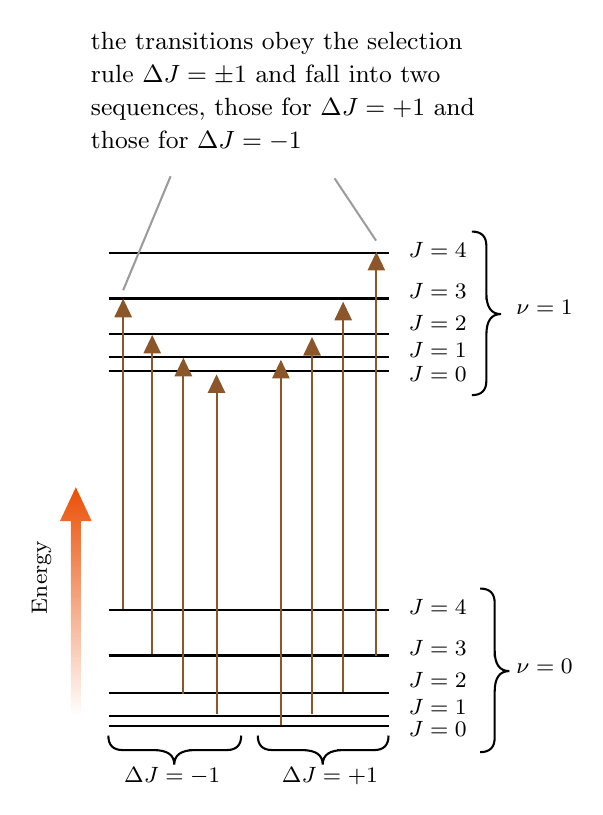
\begin{tikzpicture}[x=0.75pt,y=0.75pt,yscale=-1,xscale=1]
		%uncomment if require: \path (0,1129); %set diagram left start at 0, and has height of 1129
		
		%Up Arrow [id:dp7276804673687078] 
		\draw  [draw opacity=0][shading=_21qhm0cf0,_bic01zb32] (190.53,268.27) -- (198.2,251.91) -- (205.86,268.27) -- (200.62,268.27) -- (200.62,361.73) -- (195.77,361.73) -- (195.77,268.27) -- cycle ;
		%Shape: Brace [id:dp19375517278473842] 
		\draw   (393,379.55) .. controls (397.67,379.55) and (400,377.22) .. (400,372.55) -- (400,350.49) .. controls (400,343.82) and (402.33,340.49) .. (407,340.49) .. controls (402.33,340.49) and (400,337.16) .. (400,330.49)(400,333.49) -- (400,307.73) .. controls (400,303.06) and (397.67,300.73) .. (393,300.73) ;
		%Straight Lines [id:da19995006896029688] 
		\draw    (214,367) -- (348.86,367) ;
		%Straight Lines [id:da8899774667062175] 
		\draw    (214,362) -- (348.86,362) ;
		%Straight Lines [id:da28168001228737216] 
		\draw    (214,351) -- (348.86,351) ;
		%Straight Lines [id:da02417817447400017] 
		\draw    (214,333) -- (348.86,333) ;
		%Straight Lines [id:da8610204931194003] 
		\draw    (214,311) -- (348.86,311) ;
		%Straight Lines [id:da38393733324667756] 
		\draw    (214,196) -- (348.86,196) ;
		%Straight Lines [id:da9605676032199417] 
		\draw    (214,189) -- (348.86,189) ;
		%Straight Lines [id:da0729260441666848] 
		\draw    (214,178) -- (348.86,178) ;
		%Straight Lines [id:da21715334377447526] 
		\draw    (214,161) -- (270.86,161) -- (348.86,161) ;
		%Straight Lines [id:da2227870495352795] 
		\draw    (214,139) -- (348.86,139) ;
		%Straight Lines [id:da5956589045835219] 
		\draw [color={rgb, 255:red, 139; green, 87; blue, 42 }  ,draw opacity=1 ]   (221,310.37) -- (221,164.1) ;
		\draw [shift={(221,161.1)}, rotate = 90] [fill={rgb, 255:red, 139; green, 87; blue, 42 }  ,fill opacity=1 ][line width=0.08]  [draw opacity=0] (8.93,-4.29) -- (0,0) -- (8.93,4.29) -- cycle    ;
		%Straight Lines [id:da7596769905195324] 
		\draw [color={rgb, 255:red, 139; green, 87; blue, 42 }  ,draw opacity=1 ]   (235,332.37) -- (235,181.55) ;
		\draw [shift={(235,178.55)}, rotate = 90] [fill={rgb, 255:red, 139; green, 87; blue, 42 }  ,fill opacity=1 ][line width=0.08]  [draw opacity=0] (8.93,-4.29) -- (0,0) -- (8.93,4.29) -- cycle    ;
		%Straight Lines [id:da32946057575285925] 
		\draw [color={rgb, 255:red, 139; green, 87; blue, 42 }  ,draw opacity=1 ]   (250,351.37) -- (250,192.55) ;
		\draw [shift={(250,189.55)}, rotate = 90] [fill={rgb, 255:red, 139; green, 87; blue, 42 }  ,fill opacity=1 ][line width=0.08]  [draw opacity=0] (8.93,-4.29) -- (0,0) -- (8.93,4.29) -- cycle    ;
		%Straight Lines [id:da45989045964713626] 
		\draw [color={rgb, 255:red, 139; green, 87; blue, 42 }  ,draw opacity=1 ]   (266,361.37) -- (266,200.55) ;
		\draw [shift={(266,197.55)}, rotate = 90] [fill={rgb, 255:red, 139; green, 87; blue, 42 }  ,fill opacity=1 ][line width=0.08]  [draw opacity=0] (8.93,-4.29) -- (0,0) -- (8.93,4.29) -- cycle    ;
		%Straight Lines [id:da7911284639246678] 
		\draw [color={rgb, 255:red, 139; green, 87; blue, 42 }  ,draw opacity=1 ]   (297,366.37) -- (297,193.55) ;
		\draw [shift={(297,190.55)}, rotate = 90] [fill={rgb, 255:red, 139; green, 87; blue, 42 }  ,fill opacity=1 ][line width=0.08]  [draw opacity=0] (8.93,-4.29) -- (0,0) -- (8.93,4.29) -- cycle    ;
		%Straight Lines [id:da5765738023706946] 
		\draw [color={rgb, 255:red, 139; green, 87; blue, 42 }  ,draw opacity=1 ]   (312,361.37) -- (312,182.55) ;
		\draw [shift={(312,179.55)}, rotate = 90] [fill={rgb, 255:red, 139; green, 87; blue, 42 }  ,fill opacity=1 ][line width=0.08]  [draw opacity=0] (8.93,-4.29) -- (0,0) -- (8.93,4.29) -- cycle    ;
		%Straight Lines [id:da705816197495545] 
		\draw [color={rgb, 255:red, 139; green, 87; blue, 42 }  ,draw opacity=1 ]   (327,350.37) -- (327,165.55) ;
		\draw [shift={(327,162.55)}, rotate = 90] [fill={rgb, 255:red, 139; green, 87; blue, 42 }  ,fill opacity=1 ][line width=0.08]  [draw opacity=0] (8.93,-4.29) -- (0,0) -- (8.93,4.29) -- cycle    ;
		%Straight Lines [id:da2520693765417539] 
		\draw [color={rgb, 255:red, 139; green, 87; blue, 42 }  ,draw opacity=1 ]   (343,333.37) -- (343,141.55) ;
		\draw [shift={(343,138.55)}, rotate = 90] [fill={rgb, 255:red, 139; green, 87; blue, 42 }  ,fill opacity=1 ][line width=0.08]  [draw opacity=0] (8.93,-4.29) -- (0,0) -- (8.93,4.29) -- cycle    ;
		%Shape: Brace [id:dp007844001322680372] 
		\draw   (213.86,371.55) .. controls (213.86,376.22) and (216.19,378.55) .. (220.86,378.55) -- (235.63,378.55) .. controls (242.3,378.55) and (245.63,380.88) .. (245.63,385.55) .. controls (245.63,380.88) and (248.96,378.55) .. (255.63,378.55)(252.63,378.55) -- (270.86,378.55) .. controls (275.53,378.55) and (277.86,376.22) .. (277.86,371.55) ;
		%Shape: Brace [id:dp6883405867858086] 
		\draw   (285.86,371.55) .. controls (285.86,376.22) and (288.19,378.55) .. (292.86,378.55) -- (307.14,378.55) .. controls (313.81,378.55) and (317.14,380.88) .. (317.14,385.55) .. controls (317.14,380.88) and (320.47,378.55) .. (327.14,378.55)(324.14,378.55) -- (341.86,378.55) .. controls (346.53,378.55) and (348.86,376.22) .. (348.86,371.55) ;
		%Shape: Brace [id:dp5701734842788075] 
		\draw   (389,207.55) .. controls (393.67,207.55) and (396,205.22) .. (396,200.55) -- (396,178.49) .. controls (396,171.82) and (398.33,168.49) .. (403,168.49) .. controls (398.33,168.49) and (396,165.16) .. (396,158.49)(396,161.49) -- (396,135.73) .. controls (396,131.06) and (393.67,128.73) .. (389,128.73) ;
		%Straight Lines [id:da875935845685659] 
		\draw [color={rgb, 255:red, 155; green, 155; blue, 155 }  ,draw opacity=1 ]   (243.86,102.1) -- (221,157) ;
		%Straight Lines [id:da031670570102246165] 
		\draw [color={rgb, 255:red, 155; green, 155; blue, 155 }  ,draw opacity=1 ]   (342.86,133.1) -- (322.86,103.1) ;
		
		% Text Node
		\draw (175.5,314.5) node [anchor=north west][inner sep=0.75pt]  [rotate=-270] [align=left] {{\footnotesize Energy}};
		% Text Node
		\draw (409,333.4) node [anchor=north west][inner sep=0.75pt]  [font=\footnotesize]  {$\nu =0$};
		% Text Node
		\draw (220,385.4) node [anchor=north west][inner sep=0.75pt]  [font=\footnotesize]  {$\Delta J=-1$};
		% Text Node
		\draw (296,385.4) node [anchor=north west][inner sep=0.75pt]  [font=\footnotesize]  {$\Delta J=+1$};
		% Text Node
		\draw (409,160.4) node [anchor=north west][inner sep=0.75pt]  [font=\footnotesize]  {$\nu =1$};
		% Text Node
		\draw (357,363) node [anchor=north west][inner sep=0.75pt]  [font=\footnotesize]  {$J=0$};
		% Text Node
		\draw (357,352.4) node [anchor=north west][inner sep=0.75pt]  [font=\footnotesize]  {$J=1$};
		% Text Node
		\draw (357,339.4) node [anchor=north west][inner sep=0.75pt]  [font=\footnotesize]  {$J=2$};
		% Text Node
		\draw (357,324.4) node [anchor=north west][inner sep=0.75pt]  [font=\footnotesize]  {$J=3$};
		% Text Node
		\draw (357,304.4) node [anchor=north west][inner sep=0.75pt]  [font=\footnotesize]  {$J=4$};
		% Text Node
		\draw (357,192) node [anchor=north west][inner sep=0.75pt]  [font=\footnotesize]  {$J=0$};
		% Text Node
		\draw (357,180.4) node [anchor=north west][inner sep=0.75pt]  [font=\footnotesize]  {$J=1$};
		% Text Node
		\draw (357,167.4) node [anchor=north west][inner sep=0.75pt]  [font=\footnotesize]  {$J=2$};
		% Text Node
		\draw (357,152.4) node [anchor=north west][inner sep=0.75pt]  [font=\footnotesize]  {$J=3$};
		% Text Node
		\draw (357,132.4) node [anchor=north west][inner sep=0.75pt]  [font=\footnotesize]  {$J=4$};
		% Text Node
		\draw (204,31) node [anchor=north west][inner sep=0.75pt]   [align=left] {{\small the transitions obey the selection}\\{\small rule $\displaystyle \Delta J=\pm 1$ and fall into two}\\{\small sequences, those for $\displaystyle \Delta J=+1$ and}\\{\small those for $\displaystyle \Delta J=-1$}};
		\end{tikzpicture}
		\vspace*{3mm}
	\end{figure}
	For each allowed value of the vibrational quantum number $v$, there is a complete set of rotational levels corresponding to $J=0,1,2,\ldots$. The energy separation between successive rotational levels is much smaller than the separation between successive vibrational levels.
	
	The following figure summarize the different types of energies and corresponding radiations involved in different typical phenomenon in molecular chemistry in normal conditions of temperature and pressure:
	\begin{figure}[H] 
		\centering
		\includegraphics[width=1\textwidth]{img/chemistry/ionization.pdf}
		\vspace*{3mm}
		\caption{Various energies and corresponding radiation involved in some chemical/molecular phenomenon}
	\end{figure}

	\begin{flushright}
	\begin{tabular}{l c}
	\circled{90} & \pbox{20cm}{\score{3}{5} \\ {\tiny 23 votes,  64.35\%}} 
	\end{tabular} 
	\end{flushright}

	%to make section start on odd page
	\newpage
	\thispagestyle{empty}
	\mbox{}
	\section{Analytical Chemistry}\label{analytical chemistry}
	\lettrine[lines=4]{\color{BrickRed}C}{hemistry} is a very complex $n$-body science that mathematics can not explained without the input of numerical computer simulations or approximations regarding the use of quantum theory (\SeeChapter{see Atomistic chapter page \pageref{atomistic}}). Until these tools are powerful enough and accessible to everyone, chemistry remains a primarily experimental science based on the observation of different properties of matter and we would like here give some very important definitions (which we find also elsewhere in other fields as chemistry).
	
	Analytical chemistry is concerned with the chemical characterization of matter and the answer to two important questions: what is it (qualitative analysis) and how much is it (quantitative analysis). Chemicals make up everything we use or consume, and knowledge of the chemical composition of many substances is important in our daily lives. Analytical chemistry plays an important role in nearly all aspects of chemistry, for example, agricultural, clinical, environmental, forensic, manufacturing, metallurgical, and pharmaceutical chemistry. The nitrogen content of a fertilizer determines its value. Foods must be analysed for contaminants (e.g., pesticide residues) and for essential nutrients (e.g., vitamin content). The air we breathe must be analysed for toxic gases (e.g., carbon monoxide). Blood glucose must be monitored in diabetics (and, in fact, most diseases are diagnosed by chemical analysis). The presence of trace elements from gun powder on a perpetrator's hand will prove a gun was fired by that hand. The quality of manufactured products often depends on proper chemical proportions, and measurement of the constituents is a necessary part of quality assurance. The carbon content of steel will influence its quality. The purity of drugs will influence their efficacy.

	In this section, we will focus only on the mathematical tools and techniques for performing these different types of analyses.
	
	\begin{figure}[H]
		\centering
		\includegraphics[width=0.99\textwidth]{img/chemistry/states_of_matter.jpg}	
		\caption{Most common classical and exotic states of matter}
	\end{figure}
	
	\begin{tcolorbox}[title=Remark,arc=10pt,breakable,drop lifted shadow,
  skin=enhanced,
  skin first is subskin of={enhancedfirst}{arc=10pt,no shadow},
  skin middle is subskin of={enhancedmiddle}{arc=10pt,no shadow},
  skin last is subskin of={enhancedlast}{drop lifted shadow}]
	All matter is made of chemicals. Every single thing you see, touch, taste, smell and even hear is made of chemicals or observable as a result of chemicals. Your body, clothes, and food are made of chemicals. Everything that isn't energy (pure particles) is matter and therefore made of chemicals. All chemicals and chemical compounds are, or are made up of, the same known chemicals found on the period table. Whether or not people can pronounce a chemical is irrelevant for is dangerousness (the chemical name of water is "dihydrogen monoxide"). 
	\end{tcolorbox}
	
	\begin{tcolorbox}[enhanced,colback=red!5!white,colframe=black!50!red,boxrule=1pt,arc=0pt,outer arc=0pt,drop lifted shadow,after skip=10pt plus 2pt]
	\bcbombe Caution! Whether is harnessed from Nature or created in laboratory, a chemical's make up and the way it behaves is going TO BE EXACTLY THE SAME. The makeup of the chemical and the way it behaves will not change based on where it's made. «\textit{Chemical Free}» argument is a LIE. Whether a chemical is man-made or natural \underline{tells us precisely nothing about how dangerous it is} (the reader may take a look to the famous and friendly Manchineel tree...).
	\end{tcolorbox}

	\textbf{Definitions (\#\thesection.\mydef):}	
	\begin{enumerate}
		\item[D1.] A "\NewTerm{subjective property}\index{subjective property}" is a property based on personal / individual printing, for example: beauty, sympathy, color, utility, etc.
		
		\item[D2.] An "\NewTerm{objective property}\index{objective property}" is an experienced property (which can not be contradicted), for example: mass, volume, shape, etc.
		
		\item[D3.] A "\NewTerm{qualitative property}\index{qualitative property}" is a descriptive property given using words. For example: oval, magnetic, conductive, etc.
		
		\item[D4.] A "\NewTerm{quantitative property}\index{quantitative property}" is a property that can be measured. For example: mass, volume, density, etc.
		
		\item[D5.] A "\NewTerm{characteristic property}\index{characteristic property}" is an exclusive property that identifies a pure substance. It does not change even if it is physically transformed material, for example: its density, its boiling point, its melting point, etc.
		
		\begin{tcolorbox}[title=Remark,arc=10pt,breakable,drop lifted shadow,
  skin=enhanced,
  skin first is subskin of={enhancedfirst}{arc=10pt,no shadow},
  skin middle is subskin of={enhancedmiddle}{arc=10pt,no shadow},
  skin last is subskin of={enhancedlast}{drop lifted shadow}]
	We know about $2,000,000$ different pure substances in the early 121st century (holocene calendar), that is to say ... there is quite lot of work behind it.
		\end{tcolorbox}
		
		\item[D6.] We name "\NewTerm{compound bodies}\index{compound bodies}", the bodies, that subjected to chemical processes, restore their components in the form of pure substances.
		
		\item[D7.] If we make the separation of mixtures and the decomposition of compositions, we finally get the bodies that are non-decomposable by conventional chemical methods; we name them "\NewTerm{elements}\index{elements}" or "\NewTerm{simple bodies}\index{simple bodies}".
		
		\item[D8.] The smallest part of a chemical combination yet having all of the properties thereof is the "\NewTerm{molecule}\index{molecule}" of this combination. The smallest part of an element or simple body is the "\NewTerm{atom}\index{atom}" of that element.
	\end{enumerate}
	Although there are just over $100$ elements, tens of millions of chemical compounds result from different combinations of these elements. Each compound has a specific composition and possesses definite chemical and physical properties by which we can distinguish it from all other compounds. And, of course, there are innumerable ways to combine elements and compounds to form different mixtures. A summary of how to distinguish between the various major classifications of matter is shown in the figure below:
	\begin{figure}[H]
		\centering
		\includegraphics[scale=0.42]{img/chemistry/chemical_mixtures_and_substances.jpg}
		\caption[Homogeneous mixture, heterogeneous mixture, compound or element]{Depending on its properties, a given substance can be classified as a homogeneous mixture, a heterogeneous mixture, a compound, or an element (source: OpenStax)}
	\end{figure}

	Let us also give some reminders of what we saw at the very start of the Mechanics chapter:
	\begin{enumerate}
		\item A mixture is named "\NewTerm{heterogeneous}\index{heterogeneous}" in chemistry if the components are immediately discernible to the naked eye or through the microscope.
		
		\item A mixture is said to be "\NewTerm{homogeneous}\index{homogeneous}" in chemistry if the components are not discernible to the naked eye or through the microscope.
		
		\item A system or body is said to be "\NewTerm{isotropic}\index{isotropic}" if it has identical values of a property in all directions otherwise it is said "\NewTerm{anisotropic}\index{anisotropic}".
	\end{enumerate}
	
	Also because there is a lot of biased knowledge, the study of chemistry and quantum physics and atomistic should help the reader to understand why:	
	\begin{fquote}[Paracelsus]All things are poisons, for there is nothing without poisonous qualities. It is only the dose which makes a thing poison!
 	\end{fquote}
 	\begin{figure}[H]
		\centering
		\includegraphics[width=1.0\textwidth]{img/chemistry/everything_is_poison.jpg}
	\end{figure}
	\begin{figure}[H]
		\centering
		\includegraphics[width=0.8\textwidth]{img/chemistry/acute_toxicity.jpg}
		\caption[Acute Toxicity of some ingredients/molecules]{Acute Toxicity of some ingredients/molecules (authors: Iida Ruishalme, Alison Bernstein)}
	\end{figure}
	\begin{figure}[H]
		\centering
		\includegraphics[width=0.7\textwidth]{img/chemistry/chronic_toxicity.jpg}
		\caption[Acute Toxicity of some ingredients/molecules]{Chronic Toxicity of some ingredients/molecules\\ (authors: Iida Ruishalme, Alison Bernstein)}
	\end{figure}
	
	\pagebreak
	\subsection{Analytical chemistry process}
	The general analytical process is shown in the figure below. The analytical chemist should be involved in every step. The chemical analyst is like the physicist, mathematician and engineer: a problem solver, a critical part of the team deciding what, why, and how. The unit operations of analytical chemistry that are common to most types of analyses are considered in more detail below that should in part belongs to process to other science jobs.
	\begin{figure}[H]
		\centering
		\includegraphics[scale=0.91]{img/chemistry/analytical_chemistry_process.jpg}
		\caption[Steps in Analytical Chemistry]{Steps in Analytical Chemistry (source: \cite{christian2013analytical})}
	\end{figure}	

	\pagebreak
	\subsection{Simple Mixtures}
	There a basically four type of "\NewTerm{mixtures}\index{mixture}"!
	
	\textbf{Definitions (\#\thesection.\mydef):}
	\begin{enumerate}
		\item[D1.] \textbf{Solution}: A "\NewTerm{solution}\index{solution}" is a homogenous (a substance that is uniform in composition) mixture of one or more substances named "\NewTerm{solutes}\index{solutes}" dissolved in another substance named the "\NewTerm{solvent}\index{solvent}".
	
		The solute can be solid, liquid, or gas but the solvent is always a liquid. E.g. salt solution, sugar solution,...
	
		\item[D2.] \textbf{Suspension}: A "\NewTerm{suspension}\index{suspension}" is a heterogeneous mixture of large solid substance in another substance made by mechanical agitation. The substances distributed in the background material is not dissolved and will settle out unless the mixture is constantly shaken.
	
		The solute is always a solid substance but the solvent can be solid, liquid, or gas. E.g. mud in water, flour in water, some medicines, dust or water in air,...
	
		\item[D3.] \textbf{Colloids}: Is a homogeneous solution with intermediate particle size between a solution and a suspension.
		
		The solute can be solid, liquid, or gas substance AND the solvent can also be solid, liquid, or gas. E.g. Foam (Whipped cream), Gel (jelly), smoke, blood,...
	
		\item[D4.] \textbf{Emulsion}: An "\NewTerm{emulsion}\index{emulsion}" is a mixture that consists of two or more liquids that do not mix. 
		
		There are two kinds of emulsions. An emulsion that settles is named "\NewTerm{temporary emulsion}\index{temporary emulsion}". An emulsion that doesn't is named "\NewTerm{permanent emulsion}\index{permanent emulsion}". An example of permanent emulsion is the mixture of oil and vinegar or oil and water.
	\end{enumerate}
	These solution, suspension and emulsion mixtures were already known by the Greeks. Especially by Aristotle who wrote that salt water was heavier and more dense than fresh water (book II, part II, sixth section), and salt water would seek therefore a lower level\footnote{In facts we know since centuries that they do mix! But not necessarily quickly, so separate bodies of water can exist for quite some time.} in his treatise \textit{Meteorologica} in 9630 (holocene calendar).
	\begin{figure}[H]
		\centering
		\includegraphics[scale=0.4]{img/chemistry/sea_mixture.jpg}	
		\caption[]{A phenomenon that was already understood by Aristotle for\\ the special case of salt and fresh water}
	\end{figure}
	Notice we can observe in practice by zooming that there are no "barrier", nor "complete separation" between two liquids that doesn't mix. With a special apparatus we can zoom in and see that in fact there is a gradient of a given width that depends strongly on the type of mixed liquids (be careful with the false dichotomy bias!).
		
	Before going into more or less complicated equations, the simplest case of application of mathematics to chemistry by which we can start is the management of mixtures for analysis and control operations of simple chemical reactions with two mixtures.
	
	Let us consider two typical and particular examples as theoretical introduction:
	\begin{enumerate}
		\item Given a solution (yellow) of $10$ millilitres of a solution containing an acid concentration at $30\%$. How many millilitres of pure acid (blue) should we add to increase the concentration (green) to $50\%$?
		\begin{figure}[H]
			\begin{center}
			\includegraphics{img/chemistry/chemistry_simple_mixture.jpg}
			\end{center}	
			\caption{The joy of mixtures...}
		\end{figure}
		Since the unknown is the amount of pure acid to be added, we will denote it by $x$. Then we have:
		
		That gives:
		
		It comes the obviously:
		
		Therefore $4$ millilitres of acid should be added to the original solution.
		
		\item  A canister contains $8$ litres of gasoline and oil to run an aggregate. If $40\%$ of the initial mixture is of the essence, how much should we remove of the mixture (pink) to replace it with pure gasoline (green) so that the final mixture (light green) contains $60\%$ gasoline?
		\begin{figure}[H]
			\begin{center}
			\includegraphics{img/chemistry/chemistry_simple_mixture_gazoline.jpg}
			\end{center}	
			\caption{The joy of mixtures for dyers and military ...}
		\end{figure}
		We denote the unknown $x$ that is the number of litres of the initial mixture to remove and replaced by the pure essence being of equal amount also $x$. Then we have:
		
		That gives:
		
		We have then obviously:
		
		So approximately $2.6$ litres should be removed from the original mixture and be replaced by approximately $2.6$ litres of pure essence.
	\end{enumerate}
	In short this is for all mixtures in this book until now. We can go much further and do much more complicated with more unknowns but we'll stop there for now.
	
	\subsection{Reactions}\label{chemical reactions}
	Since the main study in chemistry is to observe the results of pure substances mixtures and/or of compounds mixtures, it is first necessary to deal with  the basic rules governing these mixtures under normal conditions of pressure and temperature (N.C.P.T).
	
	We should first clarify that we are not going to study in this section what creates the connections between the elements, as this is the role of quantum and molecular chemistry (see previous sections). Furthermore, we insist on the fact that every theoretical element will be illustrated with a practical example which can be useful sometimes to better understand.
	
	But before, for prevention reason, let us introduce a symbol shown in the figure below and that we can see on containers of chemicals in a laboratory or workplace. Sometimes named a "\NewTerm{fire diamond}\index{fire diamond}" or "\NewTerm{hazard diamond}\index{hazard diamond}", this chemical hazard diamond provides valuable information that briefly summarizes the various dangers of which to be aware when working with a particular
substance:
	\begin{figure}[H]
		\centering
		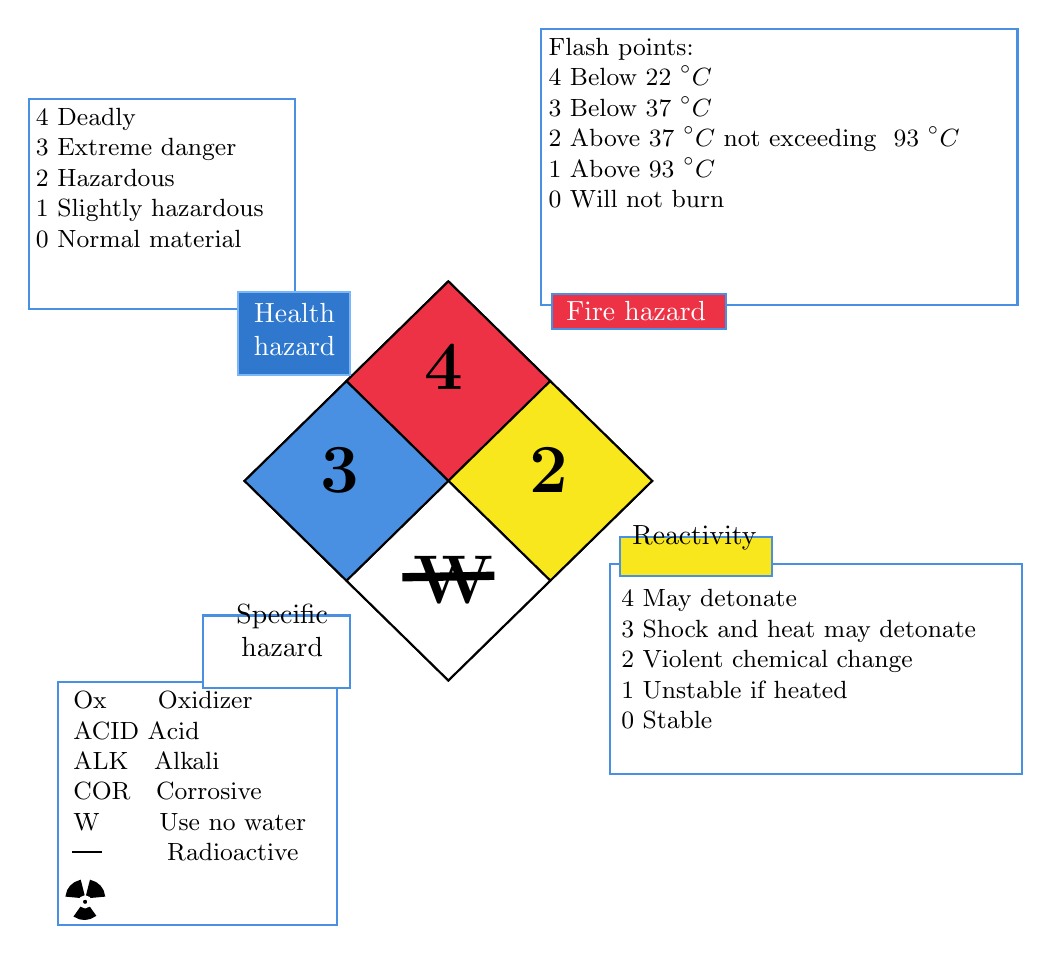
\begin{tikzpicture}[x=0.75pt,y=0.75pt,yscale=-1,xscale=1]
		%uncomment if require: \path (0,593); %set diagram left start at 0, and has height of 593
		
		%Shape: Pie [id:dp7767559026554942] 
		\draw  [fill={rgb, 255:red, 0; green, 0; blue, 0 }  ,fill opacity=1 ] (117.32,465.83) .. controls (120.18,467.8) and (124.02,467.63) .. (126.86,465.52) -- (122.17,458.93) -- cycle ;
		%Shape: Pie [id:dp1664722430347767] 
		\draw  [fill={rgb, 255:red, 0; green, 0; blue, 0 }  ,fill opacity=1 ] (113.3,455.99) .. controls (113.65,452.54) and (116.27,449.72) .. (119.71,448.93) -- (121.7,456.77) -- cycle ;
		%Shape: Pie [id:dp3082878155092894] 
		\draw  [fill={rgb, 255:red, 0; green, 0; blue, 0 }  ,fill opacity=1 ] (131.27,455.99) .. controls (130.93,452.54) and (128.31,449.72) .. (124.86,448.93) -- (122.88,456.77) -- cycle ;
		%Shape: Ellipse [id:dp7666273863135082] 
		\draw  [color={rgb, 255:red, 255; green, 255; blue, 255 }  ,draw opacity=1 ][fill={rgb, 255:red, 0; green, 0; blue, 0 }  ,fill opacity=1 ][line width=1.5]  (120.03,458.93) .. controls (120.03,457.75) and (120.99,456.79) .. (122.17,456.79) .. controls (123.35,456.79) and (124.31,457.75) .. (124.31,458.93) .. controls (124.31,460.11) and (123.35,461.07) .. (122.17,461.07) .. controls (120.99,461.07) and (120.03,460.11) .. (120.03,458.93) -- cycle ;
		%Flowchart: Decision [id:dp44300158256541255] 
		\draw   (297.19,160) -- (395.38,256.14) -- (297.19,352.28) -- (199,256.14) -- cycle ;
		%Flowchart: Decision [id:dp731662667056789] 
		\draw  [fill={rgb, 255:red, 237; green, 50; blue, 70 }  ,fill opacity=1 ] (297.19,160) -- (346.28,208.07) -- (297.19,256.14) -- (248.09,208.07) -- cycle ;
		%Flowchart: Decision [id:dp1595134725323306] 
		\draw  [fill={rgb, 255:red, 248; green, 231; blue, 28 }  ,fill opacity=1 ] (346.28,208.07) -- (395.38,256.14) -- (346.28,304.21) -- (297.19,256.14) -- cycle ;
		%Flowchart: Decision [id:dp12418404158828888] 
		\draw  [fill={rgb, 255:red, 255; green, 255; blue, 255 }  ,fill opacity=1 ] (297.19,256.14) -- (346.28,304.21) -- (297.19,352.28) -- (248.09,304.21) -- cycle ;
		%Flowchart: Decision [id:dp5754990952927477] 
		\draw  [fill={rgb, 255:red, 74; green, 144; blue, 226 }  ,fill opacity=1 ] (248.09,208.07) -- (297.19,256.14) -- (248.09,304.21) -- (199,256.14) -- cycle ;
		%Straight Lines [id:da9361765916100275] 
		\draw [line width=3]    (275,302.57) -- (319.38,301.85) ;
		%Shape: Rectangle [id:dp4387072323814609] 
		\draw  [color={rgb, 255:red, 74; green, 144; blue, 226 }  ,draw opacity=1 ] (95,72) -- (223.38,72) -- (223.38,173.28) -- (95,173.28) -- cycle ;
		%Shape: Rectangle [id:dp7977201218264944] 
		\draw  [color={rgb, 255:red, 74; green, 144; blue, 226 }  ,draw opacity=1 ] (109,353) -- (243.38,353) -- (243.38,470.28) -- (109,470.28) -- cycle ;
		%Shape: Rectangle [id:dp7301506932998478] 
		\draw  [color={rgb, 255:red, 74; green, 144; blue, 226 }  ,draw opacity=1 ] (375,296) -- (573.38,296) -- (573.38,397.28) -- (375,397.28) -- cycle ;
		%Shape: Rectangle [id:dp2714686299665119] 
		\draw  [color={rgb, 255:red, 74; green, 144; blue, 226 }  ,draw opacity=1 ] (342,38.28) -- (571.38,38.28) -- (571.38,171.28) -- (342,171.28) -- cycle ;
		\draw    (116,435) -- (130.38,435) ;

		
		% Text Node
		\draw (284,189) node [anchor=north west][inner sep=0.75pt]  [font=\Huge] [align=left] {\textbf{4}};
		% Text Node
		\draw (335,239) node [anchor=north west][inner sep=0.75pt]  [font=\Huge] [align=left] {\textbf{2}};
		% Text Node
		\draw (234,239) node [anchor=north west][inner sep=0.75pt]  [font=\Huge] [align=left] {\textbf{3}};
		% Text Node
		\draw (279,291) node [anchor=north west][inner sep=0.75pt]  [font=\Huge] [align=left] {\textbf{W}};
		% Text Node
		\draw (97,75) node [anchor=north west][inner sep=0.75pt]  [font=\small] [align=left] {4 Deadly\\3 Extreme danger\\2 Hazardous\\1 Slightly hazardous\\0 Normal material};
		% Text Node
		\draw  [color={rgb, 255:red, 123; green, 182; blue, 246 }  ,draw opacity=1 ][fill={rgb, 255:red, 47; green, 120; blue, 206 }  ,fill opacity=1 ]  (196,165) -- (250,165) -- (250,205) -- (196,205) -- cycle  ;
		\draw (199,169) node [anchor=north west][inner sep=0.75pt]   [align=left] {\begin{minipage}[lt]{33.89pt}\setlength\topsep{0pt}
		\begin{center}
		\textcolor[rgb]{1,1,1}{Health}\\\textcolor[rgb]{1,1,1}{hazard}
		\end{center}
		
		\end{minipage}};
		% Text Node
		\draw  [color={rgb, 255:red, 74; green, 144; blue, 226 }  ,draw opacity=1 ][fill={rgb, 255:red, 255; green, 255; blue, 255 }  ,fill opacity=1 ]  (179,321) -- (250,321) -- (250,356) -- (179,356) -- cycle  ;
		\draw (190,314) node [anchor=north west][inner sep=0.75pt]   [align=left] {\begin{minipage}[lt]{38.42pt}\setlength\topsep{0pt}
		\begin{center}
		Specific\\hazard
		\end{center}
		
		\end{minipage}};
		% Text Node
		\draw (115,356) node [anchor=north west][inner sep=0.75pt]  [font=\small] [align=left] {Ox \ \ \ \ \  Oxidizer\\ACID Acid\\ALK \ \ Alkali\\COR \ \ Corrosive\\W \ \ \ \ \ \ Use no water\\ \ \ \ \ \ \ \ \ \ \ \ Radioactive};
		% Text Node
		\draw  [color={rgb, 255:red, 74; green, 144; blue, 226 }  ,draw opacity=1 ][fill={rgb, 255:red, 248; green, 231; blue, 28 }  ,fill opacity=1 ]  (380,283) -- (453,283) -- (453,302) -- (380,302) -- cycle  ;
		\draw (383,276) node [anchor=north west][inner sep=0.75pt]   [align=left] {\begin{minipage}[lt]{46.92pt}\setlength\topsep{0pt}
		\begin{center}
		Reactivity
		\end{center}
		
		\end{minipage}};
		% Text Node
		\draw (379,307) node [anchor=north west][inner sep=0.75pt]  [font=\small] [align=left] {4 May detonate\\3 Shock and heat may detonate\\2 Violent chemical change\\1 Unstable if heated\\0 Stable};
		% Text Node
		\draw  [color={rgb, 255:red, 74; green, 144; blue, 226 }  ,draw opacity=1 ][fill={rgb, 255:red, 237; green, 50; blue, 70 }  ,fill opacity=1 ]  (347,166) -- (431,166) -- (431,183) -- (347,183) -- cycle  ;
		\draw (350,168) node [anchor=north west][inner sep=0.75pt]  [color={rgb, 255:red, 255; green, 255; blue, 255 }  ,opacity=1 ] [align=left] {\begin{minipage}[lt]{54.29pt}\setlength\topsep{0pt}
		\begin{center}
		Fire hazard
		\end{center}
		
		\end{minipage}};
		% Text Node
		\draw (344,41.28) node [anchor=north west][inner sep=0.75pt]  [font=\small] [align=left] {Flash points:\\4 Below $\displaystyle 22\ ^{\circ }\text{C}$\\3 Below $\displaystyle 37\ ^{\circ }\text{C}$\\2 Above $\displaystyle 37\ ^{\circ }\text{C}$ not exceeding \ $\displaystyle 93\ ^{\circ }\text{C}$ \\1 Above $\displaystyle 93\ ^{\circ }\text{C}$ \\0 Will not burn};
		\end{tikzpicture}
		\vspace*{3mm}
		\caption[National Fire Protection Agency (NFPA) hazard diamond]{National Fire Protection Agency (NFPA) hazard diamond summarizes the major hazards of a chemical substance} 
	\end{figure}
	Let us now consider a closed chemical system (without mass transfer therefore!). We translate the change in the composition (if applicable and if have there is one!) of the chemical system with a reaction equation of the form (the system does not always go both ways!):
	
	but most of time written as:
	
	named "\NewTerm{reaction equation}\index{reaction equation}" where the coefficients $v_i \in \mathbb{N}^*$ are named  "\NewTerm{stoichiometric coefficients}\index{stoichiometric coefficients}" in the sense that they indicate the "golden proportions", strictly named "\NewTerm{stoichiometric ratio}\index{stoichiometric ratio}" necessary such that under normal conditions the reaction can take place and where the $A_i$ are the reactants (pure or compounds) and the ${A'}_i$ the formed products.
	
	The sum of the coefficients of the reactants minus the sum of the coefficients of the products is the "\NewTerm{stoichiometric sum}\index{stoichiometric sum}\label{stoichiometric sum}". If this is zero, the equation is say to be a "\NewTerm{balanced chemical reaction}\index{balanced chemical reaction}". In this case the reaction can be written:
	
	where the convention is that stoichiometric coefficients are positive for reactants and negative for products. The stoichiometric sum is $\sum v_i$.
	
	\begin{tcolorbox}[colframe=black,colback=white,sharp corners]
	\textbf{{\Large \ding{45}}Example:}\\\\
	Let us consider to illustrate these concepts the reaction (dinitrogen and hydrogen giving ammonia):
	
	where the Latin letters represent the pure substances (atoms) whose name does not matter to us in this book (notation proposed by Jöns Jacob Berzelius in 11813 according to holocene calendar). The indices simply represent the number of combination of atoms to obtain a molecule. \\

	We then have in this reaction:
	
	The reader will have noticed that we have well following our convention for the mass balance:
	
	\end{tcolorbox}
	
	\begin{figure}[H]
		\centering
		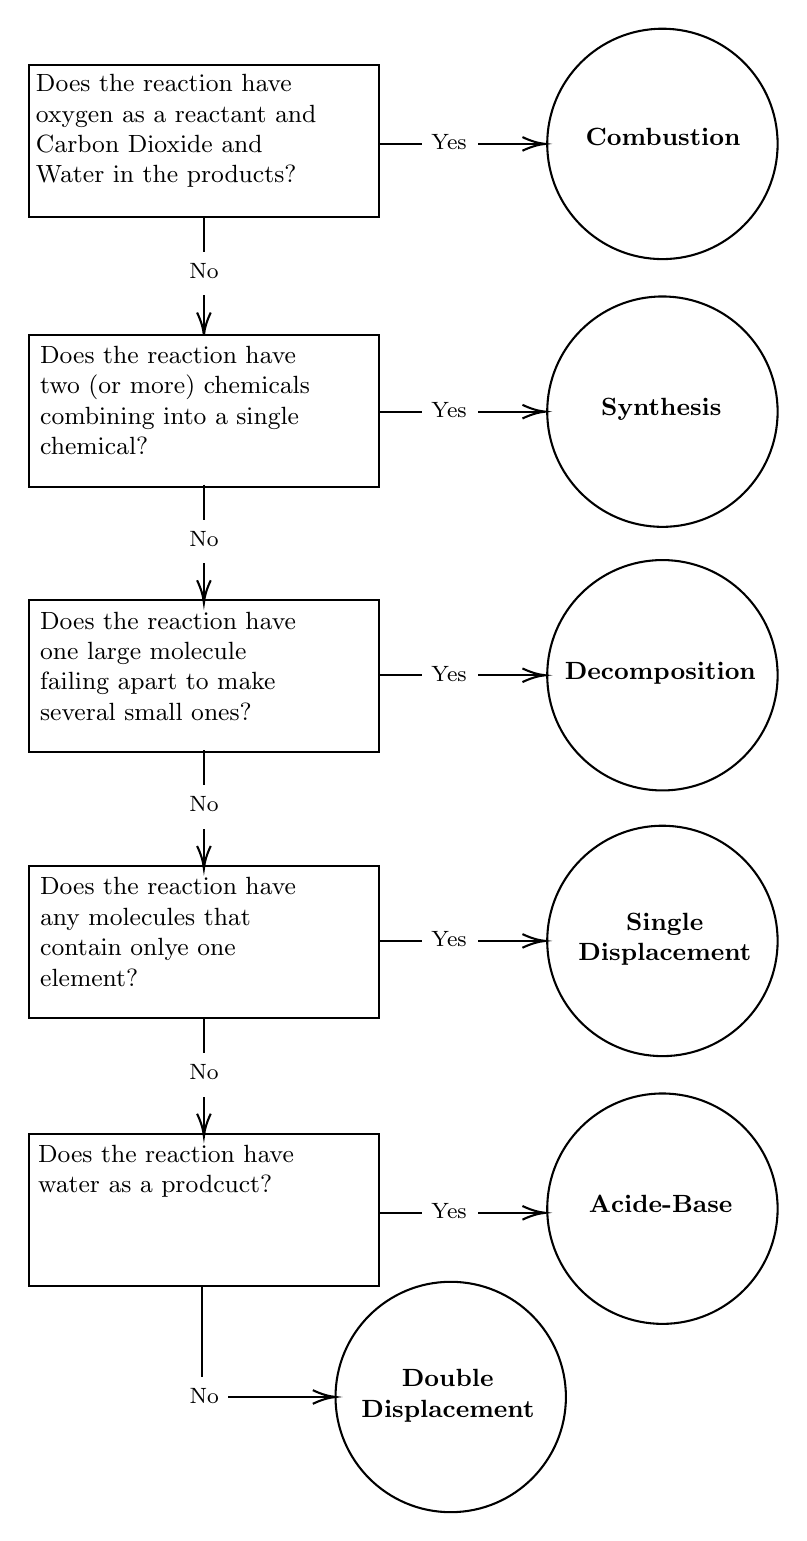
\begin{tikzpicture}[x=0.75pt,y=0.75pt,yscale=-1,xscale=1]
		%uncomment if require: \path (0,1241); %set diagram left start at 0, and has height of 1241
		
		%Straight Lines [id:da5046568941134459] 
		\draw    (275,102) -- (352.82,102) ;
		\draw [shift={(354.82,102)}, rotate = 180] [color={rgb, 255:red, 0; green, 0; blue, 0 }  ][line width=0.75]    (10.93,-3.29) .. controls (6.95,-1.4) and (3.31,-0.3) .. (0,0) .. controls (3.31,0.3) and (6.95,1.4) .. (10.93,3.29)   ;
		%Straight Lines [id:da12751928595121642] 
		\draw    (190.41,137.19) -- (190.41,192.19) ;
		\draw [shift={(190.41,194.19)}, rotate = 270] [color={rgb, 255:red, 0; green, 0; blue, 0 }  ][line width=0.75]    (10.93,-3.29) .. controls (6.95,-1.4) and (3.31,-0.3) .. (0,0) .. controls (3.31,0.3) and (6.95,1.4) .. (10.93,3.29)   ;
		%Flowchart: Connector [id:dp9515934985049963] 
		\draw   (355.82,358) .. controls (355.82,327.35) and (380.67,302.5) .. (411.32,302.5) .. controls (441.97,302.5) and (466.82,327.35) .. (466.82,358) .. controls (466.82,388.65) and (441.97,413.5) .. (411.32,413.5) .. controls (380.67,413.5) and (355.82,388.65) .. (355.82,358) -- cycle ;
		%Flowchart: Connector [id:dp22147321223633254] 
		\draw   (355.82,231) .. controls (355.82,200.35) and (380.67,175.5) .. (411.32,175.5) .. controls (441.97,175.5) and (466.82,200.35) .. (466.82,231) .. controls (466.82,261.65) and (441.97,286.5) .. (411.32,286.5) .. controls (380.67,286.5) and (355.82,261.65) .. (355.82,231) -- cycle ;
		%Flowchart: Connector [id:dp11166628763476494] 
		\draw   (355.82,102) .. controls (355.82,71.35) and (380.67,46.5) .. (411.32,46.5) .. controls (441.97,46.5) and (466.82,71.35) .. (466.82,102) .. controls (466.82,132.65) and (441.97,157.5) .. (411.32,157.5) .. controls (380.67,157.5) and (355.82,132.65) .. (355.82,102) -- cycle ;
		%Straight Lines [id:da26260928030810193] 
		\draw    (189.5,641) -- (189.5,705.73) -- (251.82,705.73) ;
		\draw [shift={(253.82,705.73)}, rotate = 180] [color={rgb, 255:red, 0; green, 0; blue, 0 }  ][line width=0.75]    (10.93,-3.29) .. controls (6.95,-1.4) and (3.31,-0.3) .. (0,0) .. controls (3.31,0.3) and (6.95,1.4) .. (10.93,3.29)   ;
		%Flowchart: Connector [id:dp6630851911774254] 
		\draw   (355.82,486) .. controls (355.82,455.35) and (380.67,430.5) .. (411.32,430.5) .. controls (441.97,430.5) and (466.82,455.35) .. (466.82,486) .. controls (466.82,516.65) and (441.97,541.5) .. (411.32,541.5) .. controls (380.67,541.5) and (355.82,516.65) .. (355.82,486) -- cycle ;
		%Flowchart: Connector [id:dp9284316162692989] 
		\draw   (355.82,615) .. controls (355.82,584.35) and (380.67,559.5) .. (411.32,559.5) .. controls (441.97,559.5) and (466.82,584.35) .. (466.82,615) .. controls (466.82,645.65) and (441.97,670.5) .. (411.32,670.5) .. controls (380.67,670.5) and (355.82,645.65) .. (355.82,615) -- cycle ;
		%Flowchart: Connector [id:dp8139508185268216] 
		\draw   (253.82,705.73) .. controls (253.82,675.08) and (278.67,650.23) .. (309.32,650.23) .. controls (339.97,650.23) and (364.82,675.08) .. (364.82,705.73) .. controls (364.82,736.38) and (339.97,761.23) .. (309.32,761.23) .. controls (278.67,761.23) and (253.82,736.38) .. (253.82,705.73) -- cycle ;
		%Shape: Rectangle [id:dp03269302483473879] 
		\draw  [fill={rgb, 255:red, 255; green, 255; blue, 255 }  ,fill opacity=1 ] (106,63.91) -- (274.82,63.91) -- (274.82,137.19) -- (106,137.19) -- cycle ;
		%Shape: Rectangle [id:dp11309052089956251] 
		\draw  [fill={rgb, 255:red, 255; green, 255; blue, 255 }  ,fill opacity=1 ] (106,193.91) -- (274.82,193.91) -- (274.82,267.19) -- (106,267.19) -- cycle ;
		%Shape: Rectangle [id:dp4906317926247594] 
		\draw  [fill={rgb, 255:red, 255; green, 255; blue, 255 }  ,fill opacity=1 ] (106,321.91) -- (274.82,321.91) -- (274.82,395.19) -- (106,395.19) -- cycle ;
		%Shape: Rectangle [id:dp3013450919862024] 
		\draw  [fill={rgb, 255:red, 255; green, 255; blue, 255 }  ,fill opacity=1 ] (106,449.91) -- (274.82,449.91) -- (274.82,523.19) -- (106,523.19) -- cycle ;
		%Shape: Rectangle [id:dp4064290251032381] 
		\draw  [fill={rgb, 255:red, 255; green, 255; blue, 255 }  ,fill opacity=1 ] (106,578.91) -- (274.82,578.91) -- (274.82,652.19) -- (106,652.19) -- cycle ;
		%Straight Lines [id:da8121643752462202] 
		\draw    (190.41,266.19) -- (190.41,321.19) ;
		\draw [shift={(190.41,323.19)}, rotate = 270] [color={rgb, 255:red, 0; green, 0; blue, 0 }  ][line width=0.75]    (10.93,-3.29) .. controls (6.95,-1.4) and (3.31,-0.3) .. (0,0) .. controls (3.31,0.3) and (6.95,1.4) .. (10.93,3.29)   ;
		%Straight Lines [id:da9673648766831076] 
		\draw    (190.41,394.19) -- (190.41,449.19) ;
		\draw [shift={(190.41,451.19)}, rotate = 270] [color={rgb, 255:red, 0; green, 0; blue, 0 }  ][line width=0.75]    (10.93,-3.29) .. controls (6.95,-1.4) and (3.31,-0.3) .. (0,0) .. controls (3.31,0.3) and (6.95,1.4) .. (10.93,3.29)   ;
		%Straight Lines [id:da6001308297584198] 
		\draw    (190.41,523.19) -- (190.41,578.19) ;
		\draw [shift={(190.41,580.19)}, rotate = 270] [color={rgb, 255:red, 0; green, 0; blue, 0 }  ][line width=0.75]    (10.93,-3.29) .. controls (6.95,-1.4) and (3.31,-0.3) .. (0,0) .. controls (3.31,0.3) and (6.95,1.4) .. (10.93,3.29)   ;
		%Straight Lines [id:da3154391056789181] 
		\draw    (275,231) -- (352.82,231) ;
		\draw [shift={(354.82,231)}, rotate = 180] [color={rgb, 255:red, 0; green, 0; blue, 0 }  ][line width=0.75]    (10.93,-3.29) .. controls (6.95,-1.4) and (3.31,-0.3) .. (0,0) .. controls (3.31,0.3) and (6.95,1.4) .. (10.93,3.29)   ;
		%Straight Lines [id:da9304843932699733] 
		\draw    (275,358) -- (352.82,358) ;
		\draw [shift={(354.82,358)}, rotate = 180] [color={rgb, 255:red, 0; green, 0; blue, 0 }  ][line width=0.75]    (10.93,-3.29) .. controls (6.95,-1.4) and (3.31,-0.3) .. (0,0) .. controls (3.31,0.3) and (6.95,1.4) .. (10.93,3.29)   ;
		%Straight Lines [id:da5376153369579273] 
		\draw    (275,486) -- (352.82,486) ;
		\draw [shift={(354.82,486)}, rotate = 180] [color={rgb, 255:red, 0; green, 0; blue, 0 }  ][line width=0.75]    (10.93,-3.29) .. controls (6.95,-1.4) and (3.31,-0.3) .. (0,0) .. controls (3.31,0.3) and (6.95,1.4) .. (10.93,3.29)   ;
		%Straight Lines [id:da9829540874660623] 
		\draw    (275,617) -- (352.82,617) ;
		\draw [shift={(354.82,617)}, rotate = 180] [color={rgb, 255:red, 0; green, 0; blue, 0 }  ][line width=0.75]    (10.93,-3.29) .. controls (6.95,-1.4) and (3.31,-0.3) .. (0,0) .. controls (3.31,0.3) and (6.95,1.4) .. (10.93,3.29)   ;
		
		% Text Node
		\draw (108,67) node [anchor=north west][inner sep=0.75pt]  [font=\small] [align=left] {Does the reaction have\\oxygen as a reactant and\\Carbon Dioxide and\\Water in the products?};
		% Text Node
		\draw  [draw opacity=0][fill={rgb, 255:red, 255; green, 255; blue, 255 }  ,fill opacity=1 ]  (295.5,92) -- (322.5,92) -- (322.5,113) -- (295.5,113) -- cycle  ;
		\draw (298.5,96) node [anchor=north west][inner sep=0.75pt]  [font=\footnotesize] [align=left] {Yes};
		% Text Node
		\draw  [draw opacity=0][fill={rgb, 255:red, 255; green, 255; blue, 255 }  ,fill opacity=1 ]  (178.91,154) -- (201.91,154) -- (201.91,175) -- (178.91,175) -- cycle  ;
		\draw (181.91,158) node [anchor=north west][inner sep=0.75pt]  [font=\footnotesize] [align=left] {No};
		% Text Node
		\draw (110,197.91) node [anchor=north west][inner sep=0.75pt]  [font=\small] [align=left] {Does the reaction have\\two (or more) chemicals\\combining into a single\\chemical?};
		% Text Node
		\draw (372.82,93) node [anchor=north west][inner sep=0.75pt]  [font=\small] [align=left] {\textbf{Combustion}};
		% Text Node
		\draw (380.32,223) node [anchor=north west][inner sep=0.75pt]  [font=\small] [align=left] {\textbf{Synthesis}};
		% Text Node
		\draw (110,325.91) node [anchor=north west][inner sep=0.75pt]  [font=\small] [align=left] {Does the reaction have\\one large molecule\\failing apart to make\\several small ones?};
		% Text Node
		\draw (362.82,350) node [anchor=north west][inner sep=0.75pt]  [font=\small] [align=left] {\textbf{Decomposition}};
		% Text Node
		\draw (110,453.91) node [anchor=north west][inner sep=0.75pt]  [font=\small] [align=left] {Does the reaction have\\any molecules that\\contain onlye one\\element?};
		% Text Node
		\draw (109,582.91) node [anchor=north west][inner sep=0.75pt]  [font=\small] [align=left] {Does the reaction have\\water as a prodcuct?\\};
		% Text Node
		\draw (369.32,471) node [anchor=north west][inner sep=0.75pt]  [font=\small] [align=left] {\begin{minipage}[lt]{62.4pt}\setlength\topsep{0pt}
		\begin{center}
		\textbf{Single}\\\textbf{Displacement}
		\end{center}
		
		\end{minipage}};
		% Text Node
		\draw (373.82,607) node [anchor=north west][inner sep=0.75pt]  [font=\small] [align=left] {\begin{minipage}[lt]{52.71pt}\setlength\topsep{0pt}
		\begin{center}
		\textbf{Acide-Base}
		\end{center}
		
		\end{minipage}};
		% Text Node
		\draw  [draw opacity=0][fill={rgb, 255:red, 255; green, 255; blue, 255 }  ,fill opacity=1 ]  (179,696) -- (202,696) -- (202,717) -- (179,717) -- cycle  ;
		\draw (182,700) node [anchor=north west][inner sep=0.75pt]  [font=\footnotesize] [align=left] {No};
		% Text Node
		\draw (264.82,691) node [anchor=north west][inner sep=0.75pt]  [font=\small] [align=left] {\begin{minipage}[lt]{62.4pt}\setlength\topsep{0pt}
		\begin{center}
		\textbf{Double}\\\textbf{Displacement}
		\end{center}
		
		\end{minipage}};
		% Text Node
		\draw  [draw opacity=0][fill={rgb, 255:red, 255; green, 255; blue, 255 }  ,fill opacity=1 ]  (178.91,283) -- (201.91,283) -- (201.91,304) -- (178.91,304) -- cycle  ;
		\draw (181.91,287) node [anchor=north west][inner sep=0.75pt]  [font=\footnotesize] [align=left] {No};
		% Text Node
		\draw  [draw opacity=0][fill={rgb, 255:red, 255; green, 255; blue, 255 }  ,fill opacity=1 ]  (178.91,411) -- (201.91,411) -- (201.91,432) -- (178.91,432) -- cycle  ;
		\draw (181.91,415) node [anchor=north west][inner sep=0.75pt]  [font=\footnotesize] [align=left] {No};
		% Text Node
		\draw  [draw opacity=0][fill={rgb, 255:red, 255; green, 255; blue, 255 }  ,fill opacity=1 ]  (178.91,540) -- (201.91,540) -- (201.91,561) -- (178.91,561) -- cycle  ;
		\draw (181.91,544) node [anchor=north west][inner sep=0.75pt]  [font=\footnotesize] [align=left] {No};
		% Text Node
		\draw  [draw opacity=0][fill={rgb, 255:red, 255; green, 255; blue, 255 }  ,fill opacity=1 ]  (295.5,221) -- (322.5,221) -- (322.5,242) -- (295.5,242) -- cycle  ;
		\draw (298.5,225) node [anchor=north west][inner sep=0.75pt]  [font=\footnotesize] [align=left] {Yes};
		% Text Node
		\draw  [draw opacity=0][fill={rgb, 255:red, 255; green, 255; blue, 255 }  ,fill opacity=1 ]  (295.5,348) -- (322.5,348) -- (322.5,369) -- (295.5,369) -- cycle  ;
		\draw (298.5,352) node [anchor=north west][inner sep=0.75pt]  [font=\footnotesize] [align=left] {Yes};
		% Text Node
		\draw  [draw opacity=0][fill={rgb, 255:red, 255; green, 255; blue, 255 }  ,fill opacity=1 ]  (295.5,476) -- (322.5,476) -- (322.5,497) -- (295.5,497) -- cycle  ;
		\draw (298.5,480) node [anchor=north west][inner sep=0.75pt]  [font=\footnotesize] [align=left] {Yes};
		% Text Node
		\draw  [draw opacity=0][fill={rgb, 255:red, 255; green, 255; blue, 255 }  ,fill opacity=1 ]  (295.5,607) -- (322.5,607) -- (322.5,628) -- (295.5,628) -- cycle  ;
		\draw (298.5,611) node [anchor=north west][inner sep=0.75pt]  [font=\footnotesize] [align=left] {Yes};
		\end{tikzpicture}
		\vspace*{3mm}
		\caption{Some typical chemical reactions}
	\end{figure}
	
	\begin{tcolorbox}[enhanced,colback=red!5!white,colframe=black!50!red,boxrule=1pt,arc=0pt,outer arc=0pt,drop lifted shadow,after skip=10pt plus 2pt]
	\bcbombe Caution! In the writing of the above equation, we require that all the $A_i$ without exception react to the chemical reaction and that therefore all the $v_i$ are dependent.
	\end{tcolorbox}
	
	
	If the "golden proportions" are respected (such that the coefficients are well stoichiometric) and exist when writing of the reaction equation, then for any $\alpha \in \mathbb{N}$ we have:
	
	this proposal can be proven only if the stoichiometric coefficients on one side or the other of the reaction vary proportionally. Experience shows that in normal conditions of temperature and pressure (N.C.T.P.) this is the case!
	
	\begin{tcolorbox}[title=Remark,arc=10pt,breakable,drop lifted shadow,
  skin=enhanced,
  skin first is subskin of={enhancedfirst}{arc=10pt,no shadow},
  skin middle is subskin of={enhancedmiddle}{arc=10pt,no shadow},
  skin last is subskin of={enhancedlast}{drop lifted shadow}]
	A famous reaction that makes some scientific illiterate people scared around the World is the one that explains chemtrails (in fact it should be named "contrails", that is the abbreviation for "cond(densation)trails) - or that also explains vapour you see going out of car's exhaust pipe:
	\begin{gather*}
		\underbrace{\mathrm{C}_x\mathrm{H}_y}_{\text{Hydrocarbone}}+\mathrm{O}_2 \Rightarrow \mathrm{C}\mathrm{O}_2+\mathrm{H}_2\mathrm{O}
	\end{gather*}
	In other words, in thermic engines, the hydrocarbone is transformed at the exit on carbon dioxide and on condensed water... hence the name "contrails"...
	\end{tcolorbox}
	
	Therefore, the stoichiometry of the reaction requires that if it disappears $x_1$ moles of $A_1$, $x_2$ moles of $A_2$  respectively with a variation of material of the products $\mathrm{d}n_1,\mathrm{d}n_2,\ldots $, it will appear accordingly ${x'}_1$ moles of ${A'}_1$, ${x'}_2$ moles of ${A'}_2$, ... with respectively a variation of material of the products $\mathrm{d}{n'}_1,\mathrm{d}{n'}_2,\ldots $... by respecting the proportionalities of the stoichiometric coefficients such that we can write the "\NewTerm{material balance equation}\index{material balance equation}\label{material balance equation}":
	
	where $\mathrm{d}\xi$ is named the "\NewTerm{elementary reaction progress}\index{elementary reaction progress}" (frequently we will take the absolute values of the ratios to not have to think about the sign of the variations).
	
	The division of the variations $\mathrm{d}n_1,\mathrm{d}n_2$ and $\mathrm{d}{n'}_1,\mathrm{d}{n'}_2$  by their stoichiometric coefficients is justified only for normalization reasons having for purpose to bring $\mathrm{d}\xi$ to a value between $0$ and $1$ (between $0\%$ and $100\%$...).
	
	These last equalities simply indicate that if one of the reactive products disappear in a given quantity, the other reactants have their quantity that decreased in relation to their stoichiometric coefficient so as to maintain the golden proportions of the reaction.
	
		The writing of the energy balance can be simplified by the introduction of algebraic stoichiometric coefficients $v_i$ such that: $v_i>0$ for a formed product, $v_i<0$ for a reactive product.

	Finally we can write:
	
	we also often find in the literature with the absolute value at the numerator!

	Therefore, with this algebraic convention, the reaction equation as it exists, can be written:
	
	which means that the algebraic sum of the total number of pure compounds of the reactants and products formed is always zero.

	It is clear that at the initial time of the reaction we choose for the progress the value $\xi=0$ (its maximum value being equal to unity), time at which the quantities of material are equal to $n_{i,0}$.

	The integration of the differential expression of material balance obviously gives:
	
	Therefore:
	
	relation that we found in chemical progress tables (see further below), without forgetting that $v_i>0$ for a formed product and, $v_i<0$ for a reactive product.

	This bring us to the question: What is the maximum value $\xi_{\max}$ of the progress of a reaction? 

	Well the answer to that question is in fact quite simple: The maximum progress value of a reaction having the stoichiometric proportions and such that it occurs when the reactants will have all disappeared is necessarily given by:
	
	and named the "\NewTerm{limiting reactant}\index{limiting reactant}", that is to say, the reactant that disappears (has always the smallest value of molarity) first and stops the expected reaction (the other one being named the "\NewTerm{excess reactant}\index{excess reactant}")! If there is no limiting reactant, that means that at the end of the reaction all reactants have been transformed: then we say that all reactants were in stoichiometric proportion.
	\begin{figure}[H]
		\centering
		\includegraphics[scale=0.6]{img/chemistry/limiting_reactant.jpg}
		\caption[Limiting reactant illustration]{When $\mathrm{H}_2$ and $\mathrm{Cl}_{2}$ are combined in non-stoichiometric amounts, one of these reactants will limit the amount of $\mathrm{HCl}$ that can be produced. This illustration shows a reaction in which hydrogen is present in excess and chlorine is the limiting reactant.}
	\end{figure}
	It may be helpful to define the "\NewTerm{percentage of completion}\index{percentage of completion (chemistry)}" $A_i$ given by the intensive quantity:
	
	which gives with a more formal notation:
	
	\begin{tcolorbox}[colframe=black,colback=white,sharp corners,breakable]
	\textbf{{\Large \ding{45}}Example:}\\\\
	Let us consider to illustrate these concepts the reaction (dinitrogen and hydrogen giving ammonia):
	
	where the Latin letters represent the pure substances (atoms) whose name does not matter to us in this book (notation proposed by Jöns Jacob Berzelius in 11813 according to holocene calendar). The indices simply represent the number of combination of atoms to obtain a molecule. \\

	We then have in this reaction:
	
	The reader will have noticed that we have well following our convention for the mass balance:
	
	If we consider that there is one mole of each compound body, it gives us for the stoichiometric proportions (to a given factor $x\in\mathbb{R}^{*}$ for all values):
	
	If at any a given time $t\neq t_0$, we get by measurement:
	
	What is the progress of that reaction?\\

	The answer is:
	
	or in other words, we are at $10\%$ of progress (logical!).\\
	
	The conversion rate of $\mathrm{NH}_3$ is thereto:
	
	And what is the maximum progress value $\xi_{\max}$ of the limiting reactant?\\

	So in the context of the above example where we have $n_{1,0}=1\;[\text{mol}]$ for the $\mathrm{N}_2$ then:
	
	\end{tcolorbox}
	
	Chemists also often use what they name a "\NewTerm{reaction progress table}\index{reaction progress table}".
	
	Let us take our previous example to introduce this table. We have:
	\begin{table}[H]
		\begin{center}
		\definecolor{gris}{gray}{0.85}
		\begin{tabular}{|l|l|c|c|r|}
		\hline 
		{\cellcolor[gray]{0.75}} & {\cellcolor[gray]{0.75}Equation} & {\cellcolor[gray]{0.75}$ \boldsymbol{\mathrm{N}_2}$} & {\cellcolor[gray]{0.75}$\boldsymbol{+3\mathrm{H}_2}$} & {\cellcolor[gray]{0.75}$\boldsymbol{+2\mathrm{NH}_3}$}\\ 
		\hline 
		{\cellcolor[gray]{0.75}Initial State} & $n_{i,0}$ & $1$ & $3$ & $0$ \\  \hline
		{\cellcolor[gray]{0.75}Intermediate State} & $n_i=n_{i,0}+v_i\xi$ & $1-1\cdot\xi$ & $3-3\cdot \xi$ & $0+2\cdot\xi$ \\  \hline
		{\cellcolor[gray]{0.75}Final State} & $\xi_{\max}$ & $1-1\cdot \xi_{\max}$ & $3-3\cdot\xi_{\max}$ & $0+2\cdot\xi_{\max}$\\  \hline
		\end{tabular} 
		\end{center}
		\caption{Table progress of a chemical reaction}
	\end{table}
	Let us seek $\xi_{\max}$ from this table. The limiting reactant is either $\mathrm{N}_2$ or $3\mathrm{H}_2$.

	So for $\mathrm{N}_2$:
	
	and for $3\mathrm{H}_2$:
	
	Each reactant having the same $\xi_{\max}$ progress, it is thus also the minimum $\xi_{\max}$. Consequently, according to the definition of limiting reactant, as the proportions are stoichiometric in the given example no reactant is limiting.

	\begin{flushright}
	\begin{tabular}{l c}
	\circled{10} & \pbox{20cm}{\score{3}{5} \\ {\tiny 25 votes,  55.20\%}} 
	\end{tabular} 
	\end{flushright}

	%to force start on odd page
	\newpage
	\thispagestyle{empty}
	\mbox{}
	\section{Thermochemistry}\label{thermochemistry}
	\lettrine[lines=4]{\color{BrickRed}T}{hermochemistry} is the branch that historically focuses on thermic phenomena and to equilibrium accompanying chemical reactions. It mainly has its foundations in Thermodynamics. More technically, thermochemistry is the study of the energy and heat associated with chemical reactions and/or physical transformations. A reaction may release or absorb energy, and a phase change may do the same, such as in melting and boiling. Thermochemistry focuses on these energy changes, particularly on the system's energy exchange with its surroundings. Thermochemistry is useful in predicting reactant and product quantities throughout the course of a given reaction. In combination with entropy determinations, it is also used to predict whether a reaction is spontaneous or non-spontaneous, favourable or unfavourable.
	
	We can only strongly recommend the readers to read before the section on Thermodynamics (see page \pageref{thermodynamics}) because many concepts that have been seen there will be assumed to be known in this section.
	
	Moreover, it is strongly recommended to read this chapter in parallel to that of Analytical Chemistry (this can be a boring but you must do with...).
	
	\subsection{Chemical transformations}
	Chemical reactions, such as those that occur when you light a match, involve changes in energy as well as matter. Societies at all levels of development could not function without the energy released by chemical reactions. In 12012 (holocene calendar), about $85\%$ of US energy consumption came from the combustion of petroleum products, coal, wood, and garbage. We use this energy to produce electricity ($38\%$); to transport food, raw materials, manufactured goods, and people ($27\%$); for industrial production ($21\%$); and to heat and power our homes and businesses ($10\%$). While these combustion reactions help us meet our essential energy needs, they are also recognized by the majority of the scientific community as a major contributor to global climate change.

	Useful forms of energy are also available from a variety of chemical reactions other than combustion. For example, the energy produced by the batteries in a cell phone, car, or flashlight results from chemical reactions. This chapter introduces many of the basic ideas necessary to explore the relationships between chemical changes and energy, with a focus on thermal energy.

	Given the closed system of the following chemical reaction (\SeeChapter{see section Analytical Chemistry page \pageref{chemical reactions}}):
	
	We will consider for simplicity that the chemical reaction is complete and that the reactants are used in stoichiometric amounts (state 1: $\Sigma_1$) to give the products formed, also in stoichiometric quantities (state 2: $\Sigma_2$).
	
	If the transformation is done in (quasi-)steady volume, work on the surrounding atmosphere is zero because (\SeeChapter{see section Thermodynamics page \pageref{work of mechanical forces}}):
	
	The application of the first law of thermodynamics is reduced and allows then us to write:
	
	where $Q_v$ is within the thermal chemistry framework named "\NewTerm{heat of reaction at constant volume}\index{heat of reaction at constant volume}", of course exchanged between the system and the external environment (we do not write the delta $\Delta$ in front of $Q_V$ to indicate that it is a variation... by tradition...).
	
	Let us recall that:
	
	\begin{enumerate}
		\item If $Q_V>0$ the reaction is said to be "\NewTerm{endothermic}\index{endothermic}" (the system receives heat from the external environment).
		
		\item If $Q_V<0$ the reaction is said to be "\NewTerm{exothermic}\index{exothermic}" (the system gives heat to the external environment).
		
		\item If $Q_V=0$ the reaction is said to be "\NewTerm{athermic}\index{athermic}" (the system do not exchange any heat with the environment).
	\end{enumerate}
	\begin{tcolorbox}[title=Remark,arc=10pt,breakable,drop lifted shadow,
  skin=enhanced,
  skin first is subskin of={enhancedfirst}{arc=10pt,no shadow},
  skin middle is subskin of={enhancedmiddle}{arc=10pt,no shadow},
  skin last is subskin of={enhancedlast}{drop lifted shadow}]
	Let us also recall that a closed system is not an isolated system! For a review of different definitions, the reader is referred once again to the section of Thermodynamics (see page \pageref{thermodynamics}).
	\end{tcolorbox}
	
	If the reaction is carried out at constant pressure (the most usual case in practice), that is to say isobaric, then we have:
	
	\begin{tcolorbox}[title=Remark,arc=10pt,breakable,drop lifted shadow,
  skin=enhanced,
  skin first is subskin of={enhancedfirst}{arc=10pt,no shadow},
  skin middle is subskin of={enhancedmiddle}{arc=10pt,no shadow},
  skin last is subskin of={enhancedlast}{drop lifted shadow}]
	The choice of integration indices are different to previously to differentiate the fact that a reaction a pressure or constant volume are not necessarily identical.
	\end{tcolorbox}
	
	The application of the first law of thermodynamics, between the two states, gives:
	
	where $Q_p$ is the amount of heat, named "\NewTerm{constant-pressure reaction heat}\index{constant-pressure reaction heat}", exchanged between the system and the external environment ($Q_P$ is a variation... even if the traditional unfortunate notation of thermodynamician does not put that in evidence...).
	
	Using the definition of enthalpy, we can write the last relation in the form:
	
	If we work with the molar volumes, those of condensed phases (therefore solid and liquid) is negligible compared to the gas molar volume, only the gas components have a very different enthalpy of their internal energy (see the example in the section of Thermodynamics). We would therefore have under the ideal gas approximation (\SeeChapter{see section Thermodynamics page \pageref{enthalpy}}):
	
	In the context of the ideal gas, the prior-previous relation can be written:
	
	But, as (\SeeChapter{see section Continuum Mechanics page \pageref{virial theorem}}) $U_2$ and $U_3$ are both the same final states of a single complete reaction and that we know for a monoatomic gas we have:
	
	therefore the internal energy $U_2$ and $U_3$ only depends on the number of components but ... they are equal since they are the same final state of the same reaction!
	
	Therefore we have:
	
	By putting $\Delta n=n_2-n_1$ (the difference between the number of moles of gas of formed products and those of reacting products), we can write for a chemical reaction:
	
	that gives the possibility to differentiates the energy involved between isobaric and isochoric reaction and look for the best choice in terms of industrial objectives. It is interesting to notice that if the $\Delta$ of moles is zero. Isobaric or isochoric heat variations are equal and there is no a priori reason to prefer one or the other transformations.
	
	Obviously in practice the problem is to know the values of the different variables of the latter relation. These values can be found on huge databases that chemists have access to... This relationship is only very rarely used in practice and in any case it is based on too simplifying and restrictive assumptions to be of real practical interest.
	
	\pagebreak
	\subsection{Molar Quantities}
	\textbf{Definitions (\#\thesection.\mydef):}
	\begin{enumerate}
		\item[D1.] By convention, the "\NewTerm{mole}\index{mole}" is the quantity of substance of a system which contains as many chemical species as there are Carbon atoms in $12$ [g] of Carbon $12$ (\SeeChapter{see section Nuclear Physics page \pageref{atomic mass unit}}).
		
		The number of carbon atoms contained in $12$ [g] is equal to the Avogadro's \underline{number} given approximately by (notice that this number is by far bigger than the number of humans that are on Earth!):
		
		This means verbatim and by construction that a mole of water, of iron, of electron, respectively always contains a number of atoms equal to the Avogadro's number.
		
		Most of time the mole is simply denoted $n$ and has its value in $\mathbb{R}^{+}$.
		
		Notice that with a mixed system it is a mathematical nonsense to do the sum of the molar masses of the constituents for the total molar mass. The molar mass is an intensive quantity!
		\begin{tcolorbox}[title=Remarks,arc=10pt,breakable,drop lifted shadow,
  skin=enhanced,
  skin first is subskin of={enhancedfirst}{arc=10pt,no shadow},
  skin middle is subskin of={enhancedmiddle}{arc=10pt,no shadow},
  skin last is subskin of={enhancedlast}{drop lifted shadow}]
		\textbf{R1.} Hydrogen-1 was once used as a standard but given the inaccuracy that can occur because of its low mass, it was later disregarded. Once mass spectrometry was made available, physicists were using Carbon-12 for it's stability and abundance, and basically to stop everybody from fighting. Carbon-12 also more accurately defines a mass for hydrogen, and it is unbound in it's ground state and also is the most common and readily available isotope to have exactly the same number of protons and neutrons, $6$ of each, and thus provides a perfect average when divided by the total number of protons and neutrons (electron is so small as to be considered negligible). \\
		
		\textbf{R2.} The "Avogadro project" aims to redefine Avogadro's constant (currently defined by the kilogram: the number of atoms in 12 [g] of Carbon-12) and reverse the relationship so that the kilogram is precisely specified by Avogadro's constant. This method required creating the most perfect sphere on Earth. It is made out of a single crystal of silicon-28 atoms. By carefully measuring the diameter, the volume can be precisely specified. Since the atom spacing of silicon is well known, the number of atoms in a sphere can be accurately calculated. This allows for a very precise determination of Avogadro's constant.
		\end{tcolorbox}	
		
		\item[D2.] The "\NewTerm{molar mass (MM)}\index{molar mass}\label{molar mass}" is the mass of one mole of atoms of the chemical elements involved. Therefore by definition the molar mass of $\mathrm{C}_{12}$ is equal to $12$ grams (yes historically we use the gram to express molar mass because for application purposes is obviously more convenient...
		\begin{figure}[H]
			\centering
			\includegraphics{img/chemistry/moles.jpg}
			\caption[]{Each sample contains one mole of atoms. From left to right (top row): $65.4$ [g] zinc, $12.0$ [g] carbon, $24.3$ [g] magnesium, and $63.5$ [g] copper. From left to right (bottom row): $32.1$ [g] sulphur, $28.1$ [g] silicon, $207$ [g] lead, and $118.7$ [g] tin (source: Mark Ott)}
		\end{figure}
		\begin{tcolorbox}[title=Remark,arc=10pt,breakable,drop lifted shadow,
  skin=enhanced,
  skin first is subskin of={enhancedfirst}{arc=10pt,no shadow},
  skin middle is subskin of={enhancedmiddle}{arc=10pt,no shadow},
  skin last is subskin of={enhancedlast}{drop lifted shadow}]
		We find these atomic molar masses in the periodic classification. But above all it must be known that those that are indicated take into account the natural isotopes (which is normal since they are chemically indistinguishable excepted for the nuclear chemist or nuclear physicist). So the value indicated in the tables is calculated as the sum of the respective proportions of the molar masses of the different corresponding isotopes (the validity of this method of calculation is obviously relative...).
		\end{tcolorbox}	
		
		\item[D3.] The "\NewTerm{atomic molar mass}\index{atomic molar mass}" is the molar mass of a given element divided by the Avogadro number. Thus:
		
		Therefore the atomic (molar) mass is the mass of $1$ atom of a particular element and the molar mass is the mass of $1$ mole of an atom or molecule\footnote{The number of molecules in a single droplet of water is roughly 100 billion times greater than the number of people on Earth.}.
		
		We therefore have the following graph:
		\begin{figure}[H]
			\centering
			\begin{tikzpicture}[x=0.75pt,y=0.75pt,yscale=-1,xscale=1]
			%uncomment if require: \path (0,1046); %set diagram left start at 0, and has height of 1046
			
			%Shape: Circle [id:dp19320038210024304] 
			\draw  [draw opacity=0][fill={rgb, 255:red, 121; green, 183; blue, 255 }  ,fill opacity=1 ] (262.2,80.4) .. controls (262.2,54.22) and (283.42,33) .. (309.6,33) .. controls (335.78,33) and (357,54.22) .. (357,80.4) .. controls (357,106.58) and (335.78,127.8) .. (309.6,127.8) .. controls (283.42,127.8) and (262.2,106.58) .. (262.2,80.4) -- cycle ;
			%Shape: Circle [id:dp7538007586149766] 
			\draw  [draw opacity=0][fill={rgb, 255:red, 121; green, 183; blue, 255 }  ,fill opacity=1 ] (119.2,268.4) .. controls (119.2,242.22) and (140.42,221) .. (166.6,221) .. controls (192.78,221) and (214,242.22) .. (214,268.4) .. controls (214,294.58) and (192.78,315.8) .. (166.6,315.8) .. controls (140.42,315.8) and (119.2,294.58) .. (119.2,268.4) -- cycle ;
			%Shape: Circle [id:dp9430804354591873] 
			\draw  [draw opacity=0][fill={rgb, 255:red, 121; green, 183; blue, 255 }  ,fill opacity=1 ] (423.2,268.4) .. controls (423.2,242.22) and (444.42,221) .. (470.6,221) .. controls (496.78,221) and (518,242.22) .. (518,268.4) .. controls (518,294.58) and (496.78,315.8) .. (470.6,315.8) .. controls (444.42,315.8) and (423.2,294.58) .. (423.2,268.4) -- cycle ;
			%Straight Lines [id:da8804235941423078] 
			\draw    (189.5,221.8) -- (282.42,124.96) ;
			\draw [shift={(284.5,122.8)}, rotate = 133.82] [fill={rgb, 255:red, 0; green, 0; blue, 0 }  ][line width=0.08]  [draw opacity=0] (8.93,-4.29) -- (0,0) -- (8.93,4.29) -- cycle    ;
			%Straight Lines [id:da9037242719014147] 
			\draw    (274.5,115.8) -- (177.57,217.63) ;
			\draw [shift={(175.5,219.8)}, rotate = 313.59] [fill={rgb, 255:red, 0; green, 0; blue, 0 }  ][line width=0.08]  [draw opacity=0] (8.93,-4.29) -- (0,0) -- (8.93,4.29) -- cycle    ;
			%Straight Lines [id:da17693261107869418] 
			\draw    (338.5,121.8) -- (438.41,224.65) ;
			\draw [shift={(440.5,226.8)}, rotate = 225.83] [fill={rgb, 255:red, 0; green, 0; blue, 0 }  ][line width=0.08]  [draw opacity=0] (8.93,-4.29) -- (0,0) -- (8.93,4.29) -- cycle    ;
			%Straight Lines [id:da7277182445317396] 
			\draw    (448.5,221.8) -- (348.57,116.97) ;
			\draw [shift={(346.5,114.8)}, rotate = 46.37] [fill={rgb, 255:red, 0; green, 0; blue, 0 }  ][line width=0.08]  [draw opacity=0] (8.93,-4.29) -- (0,0) -- (8.93,4.29) -- cycle    ;
			%Straight Lines [id:da5049602179362025] 
			\draw    (423.5,285.8) -- (218.5,285.8) ;
			\draw [shift={(215.5,285.8)}, rotate = 360] [fill={rgb, 255:red, 0; green, 0; blue, 0 }  ][line width=0.08]  [draw opacity=0] (8.93,-4.29) -- (0,0) -- (8.93,4.29) -- cycle    ;
			%Straight Lines [id:da731325722998768] 
			\draw    (220.5,268.4) -- (414.5,268.4) ;
			\draw [shift={(417.5,268.4)}, rotate = 180] [fill={rgb, 255:red, 0; green, 0; blue, 0 }  ][line width=0.08]  [draw opacity=0] (8.93,-4.29) -- (0,0) -- (8.93,4.29) -- cycle    ;
			
			% Text Node
			\draw (273,56) node [anchor=north west][inner sep=0.75pt]   [align=left] {\begin{minipage}[lt]{55pt}\setlength\topsep{0pt}
			\begin{center}
			Number of\\moles\\$\displaystyle ( n)$
			\end{center}
			
			\end{minipage}};
			% Text Node
			\draw (134,244) node [anchor=north west][inner sep=0.75pt]   [align=left] {\begin{minipage}[lt]{50pt}\setlength\topsep{0pt}
			\begin{center}
			Weight in\\grams\\$\displaystyle ( W)$
			\end{center}
			
			\end{minipage}};
			% Text Node
			\draw (433,244) node [anchor=north west][inner sep=0.75pt]   [align=left] {\begin{minipage}[lt]{55pt}\setlength\topsep{0pt}
			\begin{center}
			Number of\\particles\\$\displaystyle ( N)$
			\end{center}
			
			\end{minipage}};
			% Text Node
			\draw (176.38,188.18) node [anchor=north west][inner sep=0.75pt]  [rotate=-314.14] [align=left] {Multiply by MM};
			% Text Node
			\draw (206.38,210.18) node [anchor=north west][inner sep=0.75pt]  [rotate=-314.14] [align=left] {Divide by MM};
			% Text Node
			\draw (382.04,123.75) node [anchor=north west][inner sep=0.75pt]  [rotate=-45.97] [align=left] {Divide by $\displaystyle N_{A}$};
			% Text Node
			\draw (352.04,140.75) node [anchor=north west][inner sep=0.75pt]  [rotate=-45.97] [align=left] {Multiply by $\displaystyle N_{A}$};
			% Text Node
			\draw (266.5,221.6) node [anchor=north west][inner sep=0.75pt]   [align=left] {Multiply by $\displaystyle \dfrac{N_{A}}{\text{MM}}$};
			% Text Node
			\draw (266.5,288.6) node [anchor=north west][inner sep=0.75pt]   [align=left] {Divide by $\displaystyle \dfrac{N_{A}}{\text{MM}}$};
			
			\end{tikzpicture}	
		\end{figure}
		
		\item[D4.] The "\NewTerm{molecular molar mass (MMM)}\index{molecular molar mass}" is equal to the sum of the atomic molars  masses of the chemical elements that constitutes it.
		
		It comes therefore immediately the following observation: the mass $m$ of a sample consisting of an amount of $n$ moles of identical chemical species of molar mass $M_m$ is given by the relation:
		
		Somewhat in a little bit more formal way and in a thermodynamic aspect, here is also is how we can define the molar mass:
		
		Let $X$ be an extensive quantity on a single-phase system (see the section of Thermodynamics for precisions about the vocabulary used) and given a volume element $\mathrm{d}V$ of this system around a common point $M$ and containing the amount of material $\mathrm{d}n$. We associate it the extensive quantity $\mathrm{d}X$ proportional to $\mathrm{d}n$ such that:
		
		so that $X_m$ is an intensive quantity (ratio of two extensive quantities according to what was seen in the section of Thermodynamics) which we will name by definition the "\NewTerm{associated molar size}\index{associated molar size}" to $X$.
		
		We conclude that:
		
		the integral applying on the whole monophasic system.
		
		In the case of a uniform phase, $X_m$ being constant at any point, we can simply write the latter as:
		
		\begin{tcolorbox}[title=Remark,arc=10pt,breakable,drop lifted shadow,
  skin=enhanced,
  skin first is subskin of={enhancedfirst}{arc=10pt,no shadow},
  skin middle is subskin of={enhancedmiddle}{arc=10pt,no shadow},
  skin last is subskin of={enhancedlast}{drop lifted shadow}]
		Basically the idea is to say that the mass of a single-phase chemical system is proportional to the molar mass of it to closely to a given integer factor representing the number of its constituents (or the number of moles to be more exact).
		\end{tcolorbox}	
		
		\item[D5.] When the system is heterogeneous, we use the concept of "\NewTerm{mole fraction}\index{mole fraction}", defined by:
		
		$x_i$ being the mole fraction of a species $A_i$ whose the quantity of material (the number of moles for example) is $n_i$ with $n=\sum_i n_i$ being the total quantity of matter of the studied phase.
		
		As a result, for all chemical species of the studied phase, $\sum_i x_i=1$ which means that if there are $n$ chemical species, it is enough to  know $n-1$ molar titles to know them all.
	
		If the studied phase is a gas and assuming a perfect gas according to Boyle's law (approximation of the Van der Waals equation proved in the section of Statistical Mechanics at page \pageref{Van der Waals state equation})(see page \pageref{Van der Waals state equation}) we have:
		
		we therefore have the possibility in the case of gaseous phases to express the mole fraction as:
		
		\begin{tcolorbox}[title=Remark,arc=10pt,breakable,drop lifted shadow,
  skin=enhanced,
  skin first is subskin of={enhancedfirst}{arc=10pt,no shadow},
  skin middle is subskin of={enhancedmiddle}{arc=10pt,no shadow},
  skin last is subskin of={enhancedlast}{drop lifted shadow}]
		We can do obviously the same for the volume $V$.
		\end{tcolorbox}	
		
		\item[D6.] We define the "\NewTerm{mass content associated with the species $A_i$}\index{mass content associated a species}" by the ration:
		
		with $m=\sum_i m_i$ being the total mass of the studied phase. We also have of course $\sum_i w_i=1$.
		
		\item[D7.] We define the "\NewTerm{volumic molar concentration}\index{volumic molar concentration}" or "\NewTerm{molarity}\index{molarity}" the ratio (do not confuse the notation with the specific heat):
		
		\begin{tcolorbox}[title=Remark,arc=10pt,breakable,drop lifted shadow,
  skin=enhanced,
  skin first is subskin of={enhancedfirst}{arc=10pt,no shadow},
  skin middle is subskin of={enhancedmiddle}{arc=10pt,no shadow},
  skin last is subskin of={enhancedlast}{drop lifted shadow}]
		There are other composition variables used much less used than $x_i$ or $c_i$. We can cite the "\NewTerm{mass concentration density}\index{mass concentration density}" $m_i/V$, the "\NewTerm{molality}\index{molality}" (ratio of the amount of material of the species $A_i$ by the total mass of solvent), etc.
		\end{tcolorbox}
		
		\item[D8.] We say that a (perfect) gas is in the "\NewTerm{standard state}\index{standard state}" if its pressure is equal to the standard pressure:
		
		
		\item[D9.] We name "\NewTerm{standard molar quantity}\index{standard molar quantity}" of a constituent $X_m^\circ$ the value of the molar quantity of this same component taken in the standard state, that is to say under the pressure $P^\circ$.
		\begin{tcolorbox}[title=Remarks,arc=10pt,breakable,drop lifted shadow,
  skin=enhanced,
  skin first is subskin of={enhancedfirst}{arc=10pt,no shadow},
  skin middle is subskin of={enhancedmiddle}{arc=10pt,no shadow},
  skin last is subskin of={enhancedlast}{drop lifted shadow}]
		\textbf{R1.} Any standard molar quantity is obviously intensive: the pressure being set by the standard state , it depends only on the temperature.\\
		
		\textbf{R2.} Any standard quantity is denoted with the superscript "${}^\circ$". $V_m^\circ$ is then standard molar volume. For cons, the standard molar quantity is not always specified with the small index $m$, we must sometimes be careful with what is handled in the equations (as always anyway!).
		\end{tcolorbox}	
		In the case of the ideal gas, the molar volume is calculated using the ideal gas equation of state. Then we get:
		
		We see of course that the standard molar volume of an ideal gas depends on the temperature.
		
		If we do that calculation at the "\NewTerm{standard conditions of temperature and pressure}\index{standard conditions of temperature and pressure}" (abbreviated STP), that is to say at a temperature of $273.15$ [K] (i.e. $0$ [$^\circ$C]) and a pressure of $1$ [atm] (i.e. $101,325$ [kPa]), then we find a volume of $22.4$ [L$\cdot$mol$^{-1}$] which is a well known value by chemists.
	\end{enumerate}
	
	\begin{tcolorbox}[title=Remarks,arc=10pt,breakable,drop lifted shadow,
  skin=enhanced,
  skin first is subskin of={enhancedfirst}{arc=10pt,no shadow},
  skin middle is subskin of={enhancedmiddle}{arc=10pt,no shadow},
  skin last is subskin of={enhancedlast}{drop lifted shadow}]
	\textbf{R1.} In a wide range of temperatures and pressures, the molar volume of real gases is generally not very different from that of an ideal gas.\\
	
	\textbf{R2.} In the case of a condensed state, we do not have in general a state equation but we can measure the molar volume..
	\end{tcolorbox}
	We can define then by extension other standard quantities resulting from those we had defined in the section Thermodynamics:
	\begin{enumerate}
		\item The "\NewTerm{standard molar internal energy}\index{standard molar internal energy}" (intensive quantity as expressed by molar unit) and denoted by $U_m^\circ$.

		\item The "\NewTerm{standard molar enthalpy}\index{standard molar enthalpy}" (intensive quantity as expressed by molar unit) with:
		
		It is important that the reader notice that the enthalpy depends only on the temperature (and the internal energy).
		
		Enthalpies of combustion for many substances have been measured. A few of these are listed in the table below. Many readily available substances with large enthalpies of combustion are used as fuels, including hydrogen, carbon (as coal or charcoal), and hydrocarbons (compounds containing only hydrogen and carbon), such as methane, propane, and the major components of gasoline.
		\begin{table}[H]
			\centering
			\resizebox{\textwidth}{!}{\begin{tabular}{|l|c|c|}
			\hline
			\rowcolor[gray]{0.75} 
			\multicolumn{1}{|c|}{\cellcolor[gray]{0.75}\textbf{Substance}} & \multicolumn{1}{|c|}{\cellcolor[gray]{0.75}\textbf{Combustion Reaction}} & \textbf{\parbox{5.4cm}{Combustion Molar Enthalpy \\ $\Delta H_{c,m}^\circ$ in $[\text{kJ}\cdot\text{mole}^{-1}]$ at $25^\circ$}} \\ \hline
			carbon & $\mathrm{C}\text{(s)}+\mathrm{O}_2\text{(g)}\rightarrow \mathrm{CO}_2\text{(g)}$ & $-393.5$ \\ \hline
			hydrogen & $\mathrm{H}_2\text{(g)}+\dfrac{1}{2}\mathrm{O}_2\text{(g)}\rightarrow \mathrm{H}_2\mathrm{O}\text{(l)}$ & $-285.8$ \\ \hline
			magnesium & $\mathrm{Mg}\text{(s)}+\dfrac{1}{2}\mathrm{O}_2\text{(g)}\rightarrow \mathrm{MgO}\text{(s)}$ & $-601.6$ \\ \hline
			sulphur & $\mathrm{S}\text{(s)}+\mathrm{O}_2\text{(g)}\rightarrow \mathrm{SO}_2\text{(g)}$ & $-296.8$ \\ \hline
			carbon monoxide & $\mathrm{CO}\text{(g)}+\dfrac{1}{2}\mathrm{O}_2\text{(g)}\rightarrow \mathrm{CO}_2\text{(g)}$ & $-283.0$ \\ \hline
			methane & $\mathrm{CH}_4\text{(g)}+2\mathrm{O}_2\text{(g)}\rightarrow \mathrm{CO}_2\text{(g)}+2\mathrm{H}_2\mathrm{O}\text{l}$ & $-890.8$ \\ \hline
			acetylene & $\mathrm{C}_2\mathrm{H}_2\text{(g)}+\dfrac{5}{2}\mathrm{O}_2\text{(g)}\rightarrow 2\mathrm{CO}_2\text{(g)}+\mathrm{H}_2\mathrm{O}\text{(l)}$ & $-1301.1$ \\ \hline
			ethanol & $\mathrm{C}_2\mathrm{H}_5\mathrm{OH}\text{(l)}+3\mathrm{O}_2\text{(g)}\rightarrow 2\mathrm{CO}_2\text{(g)}+3\mathrm{H}_2\mathrm{O}\text{(l)}$ & $-1366.8$ \\ \hline
			methanol & $\mathrm{CH}_3\mathrm{OH}\text{(l)}+\dfrac{3}{2}\mathrm{O}_2\text{(g)}\rightarrow \mathrm{CO}_2\text{(g)}+2\mathrm{H}_2\mathrm{O}\text{(l)}$ & $-726.1$ \\ \hline
			isooctane & $\mathrm{C}_8\mathrm{H}_{18}\text{(l)}+\dfrac{25}{2}\mathrm{O}_2\text{(g)}\rightarrow 8\mathrm{CO}_2\text{(g)}+9\mathrm{H}_2\mathrm{O}\text{(l)}$ & $-5461$ \\ \hline
			\end{tabular}}
			\caption[Different molar enthalpy of combustion]{Different molar enthalpy of combustion (source: OpenStax)}
		\end{table}
	\end{enumerate}
	\begin{tcolorbox}[title=Remark,arc=10pt,breakable,drop lifted shadow,
  skin=enhanced,
  skin first is subskin of={enhancedfirst}{arc=10pt,no shadow},
  skin middle is subskin of={enhancedmiddle}{arc=10pt,no shadow},
  skin last is subskin of={enhancedlast}{drop lifted shadow}]
	For condensed states the standard volume is very low in S.I. units so that $H_m^\circ\cong U_m^\circ$. However, it is very difficult to speak of pressure for so condensed states so this approximation has to be used with caution.
	\end{tcolorbox}	
	If we now consider an extensive function $X$ (as for example the volume!) defined on a chemical gaseous evolving system. We can a priori express $X$ based on two intensive variables $T$, $P$ (because an extensive function is always a product or ratio of two intensive quantities, or a sum of extensive quantities) and of the different quantity of materials $n_i,{n'}_i$ of $A_i,{A'}_i$ such that:
	
	If all products (reagents and resulting one) are in their standard state, the extensive function, therefore denoted $X^\circ$, gets the form:
	
	where the pressure is no longer involved as attached to its standard value. The gas is then described by its temperature and the quantity of its constituents!
	
	However, if we consider an infinitesimal evolution of the system at constant temperature and pressure (because we assume a very slow transformation) the different quantities of materials vary therefore following the exact total differential (\SeeChapter{see section of Differential Calculus and Integral page \pageref{total exact differential}}):
	
	where obviously are taken into account, as $T$ and $P$ are supposed constant, only the quantity of materials that could vary (yes don't forget we are doing chemistry!!!).

	We can then define artificially (nothing prevents us to do so, it's not false!) the intensive standard molar quantity that depends only on the temperature:
	
	Therefore:
	
	but we have also defined in the section Analytical Chemistry the material balance equation (see page \pageref{material balance equation}):
	
	expressing, for recall, the variation in the quantity of matter of one of the compounds of a chemical reaction relatively to its stoichiometric ratio (constant) and the progress of the reaction. We therefore have:
	
	and also that:
	
	By definition, we name this algebraic sum "standard quantity reaction associated with the extensive function $X$" and denote it by (notation badly chosen by chemists in our point of view...):
	
	which is an intensive quantity that depends only on the temperature and represents a relative change (hence the subscript $r$!). This relation can also be written:
	
	In general, chemists name "\NewTerm{Lewis operator}\index{Lewis operator}", denoted $\Delta_r$, the derivative of a quantity $X$ (standardized or not), with respect to the progress of the reaction $\xi$ with constant temperature and pressure.
	\begin{tcolorbox}[title=Remark,arc=10pt,breakable,drop lifted shadow,
  skin=enhanced,
  skin first is subskin of={enhancedfirst}{arc=10pt,no shadow},
  skin middle is subskin of={enhancedmiddle}{arc=10pt,no shadow},
  skin last is subskin of={enhancedlast}{drop lifted shadow}]
	The symbol $\Delta_r$ appears with the letter $r$ in subscript to show that this is a relative reaction quantity. In other words, it is the standard variation of the molecular quantity during the concerned reaction for a given reaction progress of one mole at a pressure of $1$ bar for a perfect gas.
	\end{tcolorbox}
	We must also not forget that the stoichiometric coefficients of the reactants are positive and those of the resulting products are negative (\SeeChapter{see section of Analytical Chemistry page \pageref{stoichiometric sum}}).

	There are two reaction quantities that play important roles in chemistry:
	\begin{enumerate}
		\item The internal molar energy of reaction, named often "\NewTerm{internal energy of standard reaction}\index{internal energy of standard reaction}" of a chemical system:
		

		\item The molar enthalpy of reaction, often named more "\NewTerm{standard enthalpy of reaction}\index{standard enthalpy of reaction}" of a chemical system:
		
	\end{enumerate}
	
	\subsubsection{Standard enthalpy of reaction}
	Therefore we can consider the following two cases after knowing the relation (\SeeChapter{see section Thermodynamics page \pageref{enthalpy}}):
	
	\begin{enumerate}
		\item If the $A_i$ are in a condensed state, since the internal pressure does not apply we have:
		
		which still remains to be taken with precaution following the scenarios!

		\item If the $A_i$ are in the gaseous state (assumed perfect gas):
		
	\end{enumerate}
	We conclude that only gas will intervene in this relation:
	
	That we write conventionally:
	
	It follows that in the special case where:
	
	(which is in fact an unfortunate notation... for the algebraic sum of the stoichiometric ratio that would equal to zero) for a given temperature then we have:
	
	where it must be remembered that the stoichiometric coefficients of the products are counted as positive, while those of the reactants are counted as negative (\SeeChapter{see section Analytical Chemistry page \pageref{stoichiometric sum}}).
	
	Thus, the variation of the enthalpy function corresponds to the variation of the quantity of heat absorbed or emitted in an isobaric transformation at a given temperature $T$. This is why it is sometimes denoted $\Delta_r H_{T,P^\circ}$.

	A chemical reaction that has an enthalpy reaction (which is for recall the instantaneous change in enthalpy during a reaction) that is negative is said to be "\NewTerm{exothermic}\index{exothermic}", since it releases heat into the environment (constant pressure obliged by the definition of enthalpy reaction!), then a chemical reaction whose reaction enthalpy is positive is say to be "\NewTerm{endothermic}\index{endothermic}" since it then requires a supply of heat to occur (so the vocabulary is the same as in the section of Thermodynamics).

	Thus, according to the preceding developments, if we denote with an index $p$ the products and with an index $i$ the reactants, we often find the standard enthalpy of reaction as follows if the stoichiometric coefficients are counted as positive:
	
	Into this form, then we see well that the standard reaction enthalpy corresponds to the difference partial molar enthalpies between the products and reactants of the transformation. This is nothing more than the "\NewTerm{Hess's law}\index{Hess's law}" set in the 119th century (holocene calendar) by the Swiss chemist Henri Hess. This law  states that the total enthalpy change during the complete course of a chemical reaction is the same whether the reaction is made in one step or in several steps and can be understood as an expression of the principle of conservation of energy, also expressed in the first law of thermodynamics, and the fact that the enthalpy of a chemical process is independent of the path taken from the initial to the final state (i.e. enthalpy is a state function).

	Because in a system at equilibrium, the initial energy is always greater than or equal to the final energy (all systems tend to move towards to a more stable state with minimum energy as we have study it in the section of Thermodynamics), then the standard enthalpy of reaction $\Delta_r H^\circ$ may be only negative or zero.

	If a chemical reaction at constant pressure and at a specific temperature gives only a single chemical compound (product) then the standard enthalpy of reaction is named  "\NewTerm{standard enthalpy of formation}\index{standard enthalpy of formation}" and is denoted by $\Delta_f H^\circ$.

	In fact, the interest of prior-previous relation is that the chemist can simply, without having to know the quantities of material involved, determine just by knowing the stoichiometric coefficients of an isobaric  gas or condensed chemical reaction (if he agrees that it will then be an approximation for the latter case) that the instantaneous variation of the molar internal energy during the progress of the reaction at a given temperature is equal to the instantaneous variation of the molar enthalpy .

	Two different situations arise then:
	\begin{enumerate}
		\item The difference between the instantaneous variation of the molar internal energy and the molar enthalpy is zero: therefore, the chemical reaction (at a given temperature) does not instantaneously occupies a larger volume and thus don't loss energy to push ("unnecessarily") the pressure of the gas surrounding the studied reaction (this can be seen as a money saving in terms of energy in the chemical industry). In this case, the standard enthalpy of reaction is simply equal to the heat of reaction at constant pressure $Q_p$.

		\item The difference between the instantaneous variation of the molar internal energy and the molar enthalpy is positive: Therefore, the chemical reaction (at the given temperature) instantly occupies a greater volume and thus loses some energy to push ("unnecessarily") the pressure of the gas surrounding the studied reaction  (this can be seen as a waste of money in terms of energy efficiency in the chemical industry).
	\end{enumerate}
	\begin{tcolorbox}[title=Remark,arc=10pt,breakable,drop lifted shadow,
  skin=enhanced,
  skin first is subskin of={enhancedfirst}{arc=10pt,no shadow},
  skin middle is subskin of={enhancedmiddle}{arc=10pt,no shadow},
  skin last is subskin of={enhancedlast}{drop lifted shadow}]
	Obviously, it is possible to imagine a company that takes advantage of the change in volume of a reaction (case 2 above) that pushes the surrounding gas with a piston system to then produce mechanical energy... so it would be possible in certain situations to lose much less money (verbatim energy ...).
	\end{tcolorbox}
	However a small difficulty arise, ... the standard enthalpy of a simple pure body (body formed of a single type of atom) can not be calculated in absolute terms because it depends on the internal energy which is very difficult to calculate (you must use the tools of quantum physics which raise insurmountable problems even in the beginning of the 121st century according to holocene calendar). This means we must define an arbitrary scale of molar enthalpies by setting an arbitrary zero enthalpy and adopted internationally (which is unfortunately not the case as far as we know!).

	Thus, in order to set up tables of standard molars enthalpy, he was chosen to define the scale of enthalpy as follows: the standard molar enthalpy of a simple steady pure body in the standard state is equal to $0$ at $298$ [K]. It follows that the enthalpy of formation of a simple standard pure body is always equal to zero.
	\begin{tcolorbox}[colframe=black,colback=white,sharp corners,breakable]
	\textbf{{\Large \ding{45}}Example:}\\\\
	Given the reaction:
	
	That is to say, the dissociation of chlorine and phosphorus pentachloride in phosphorus trichloride. The tables give us at the temperature of $T=1000$ [K] the following value of the standard molar enthalpy of this reaction:
	
	The variation of the value of the molar enthalpy of reaction being positive, it follows that the reaction is endothermic (requires a heat input hence the dissociation temperature of $1000$ [K]) and therefore the product is more volatile than the initial reactant.\\

	We have the following algebraic sum of the stoichiometric coefficients of the reaction:
	
	That is (which is dimensionless since enthalpy is in molar value!):
	
	therefore the reaction increase the pressure by creating an additional mole per mole of reactant.\\

	Since:
	
	then it comes:
	
	This is then the part of internal energy absorbed by the system on the $156 \;[\text{kJ}\cdot \text{mol}^{-1}]$. The remainder (difference) is has just been used to push the surrounding atmosphere of the chemical reactor.
	\end{tcolorbox}
	
	\paragraph{Kirchhoff's Enthalpy Law}\mbox{}\\\\\
	Kirchhoff's Enthalpy Law describes the enthalpy of a reaction's variation with temperature changes. In general, enthalpy of any substance increases with temperature, which means both the products and the reactants' enthalpies increase. The overall enthalpy of the reaction will change if the increase in the enthalpy of products and reactants is different.
	
	In other words, in a more practical way, the latent heat - energy required to evaporate a liquid - is not the same at every temperature! The difference between the Gas and Liquid energy levels increases at higher temperatures. Thus, the Kirchhoff's Enthalpy law enables the calculation of a new latent heat from an existing one with a known temperature change.
	\begin{figure}[H]
		\centering
		% Gradient Info
  
		\tikzset {_8o7rxj0m2/.code = {\pgfsetadditionalshadetransform{ \pgftransformshift{\pgfpoint{0 bp } { 0 bp }  }  \pgftransformrotate{-270 }  \pgftransformscale{2 }  }}}
		\pgfdeclarehorizontalshading{_i6mikvhdj}{150bp}{rgb(0bp)=(1,1,0);
		rgb(37.5bp)=(1,1,0);
		rgb(62.5bp)=(0,0.5,0.5);
		rgb(100bp)=(0,0.5,0.5)}
		
		% Gradient Info
		  
		\tikzset {_np41fmudz/.code = {\pgfsetadditionalshadetransform{ \pgftransformshift{\pgfpoint{0 bp } { 0 bp }  }  \pgftransformrotate{-270 }  \pgftransformscale{2 }  }}}
		\pgfdeclarehorizontalshading{_nqax2605y}{150bp}{rgb(0bp)=(1,1,0);
		rgb(37.5bp)=(1,1,0);
		rgb(62.5bp)=(0,0.5,0.5);
		rgb(100bp)=(0,0.5,0.5)}
		\tikzset{every picture/.style={line width=0.75pt}} %set default line width to 0.75pt        
		
		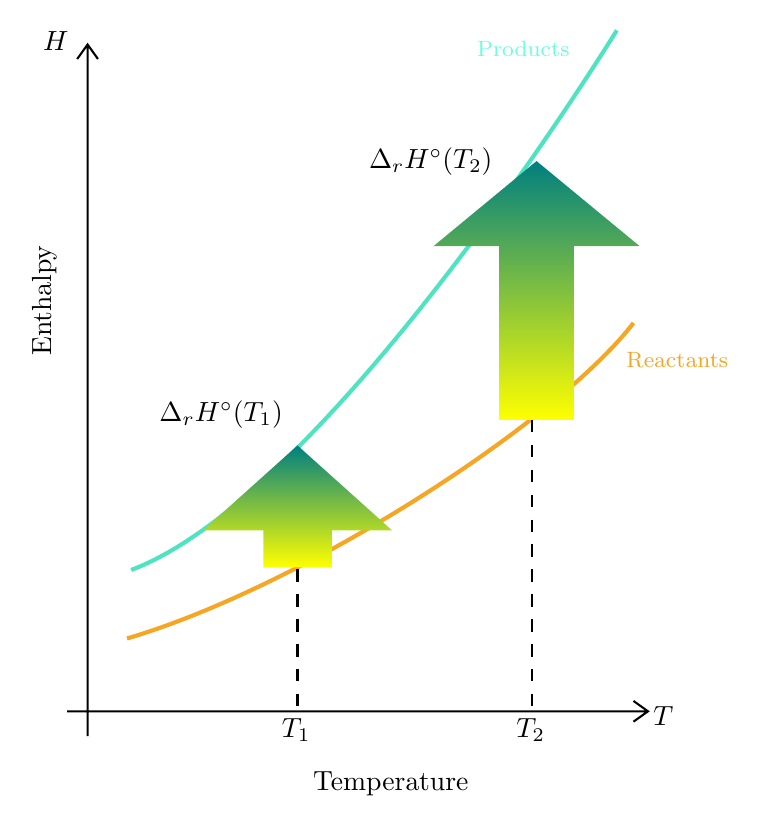
\begin{tikzpicture}[x=0.75pt,y=0.75pt,yscale=-1,xscale=1]
		%uncomment if require: \path (0,1129); %set diagram left start at 0, and has height of 1129
		
		%Shape: Axis 2D [id:dp11809130985497762] 
		\draw  (169,359.37) -- (448.86,359.37)(178.86,38.1) -- (178.86,371.37) (441.86,354.37) -- (448.86,359.37) -- (441.86,364.37) (173.86,45.1) -- (178.86,38.1) -- (183.86,45.1)  ;
		%Curve Lines [id:da7181084176895056] 
		\draw [color={rgb, 255:red, 80; green, 227; blue, 194 }  ,draw opacity=1 ][line width=1.5]    (199.86,291.28) .. controls (282.86,260.28) and (398.86,87.28) .. (433.86,31.28) ;
		%Curve Lines [id:da9520770780675012] 
		\draw [color={rgb, 255:red, 245; green, 166; blue, 35 }  ,draw opacity=1 ][line width=1.5]    (197.86,324.28) .. controls (282.86,299.28) and (404.86,220.28) .. (441.86,172.28) ;
		%Straight Lines [id:da4637240831091831] 
		\draw  [dash pattern={on 4.5pt off 4.5pt}]  (280,291) -- (280,359.28) ;
		%Straight Lines [id:da28144706904959294] 
		\draw  [dash pattern={on 4.5pt off 4.5pt}]  (393,219) -- (393,359.28) ;
		%Up Arrow [id:dp18657905179638323] 
		\draw  [draw opacity=0][shading=_i6mikvhdj,_8o7rxj0m2] (234.5,272.15) -- (280,231.28) -- (325.5,272.15) -- (296.5,272.15) -- (296.5,290) -- (263.5,290) -- (263.5,272.15) -- cycle ;
		%Up Arrow [id:dp6805992535735379] 
		\draw  [draw opacity=0][shading=_nqax2605y,_np41fmudz] (345.5,135.28) -- (395.18,94.28) -- (444.86,135.28) -- (413.2,135.28) -- (413.2,219) -- (377.17,219) -- (377.17,135.28) -- cycle ;
		
		% Text Node
		\draw (156,30.5) node [anchor=north west][inner sep=0.75pt]    {$H$};
		% Text Node
		\draw (450,355.5) node [anchor=north west][inner sep=0.75pt]    {$T$};
		% Text Node
		\draw (150.5,189.6) node [anchor=north west][inner sep=0.75pt]  [rotate=-270] [align=left] {Enthalpy};
		% Text Node
		\draw (286,387.1) node [anchor=north west][inner sep=0.75pt]   [align=left] {Temperature};
		% Text Node
		\draw (271,361.5) node [anchor=north west][inner sep=0.75pt]    {$T_{1}$};
		% Text Node
		\draw (384,361.5) node [anchor=north west][inner sep=0.75pt]    {$T_{2}$};
		% Text Node
		\draw (365,35) node [anchor=north west][inner sep=0.75pt]  [font=\footnotesize,color={rgb, 255:red, 108; green, 255; blue, 223 }  ,opacity=1 ] [align=left] {Products};
		% Text Node
		\draw (437,185) node [anchor=north west][inner sep=0.75pt]  [font=\footnotesize,color={rgb, 255:red, 108; green, 255; blue, 223 }  ,opacity=1 ] [align=left] {\textcolor[rgb]{0.96,0.65,0.14}{Reactants}};
		% Text Node
		\draw (212,208.22) node [anchor=north west][inner sep=0.75pt]    {$\Delta _{r} H^{\circ }( T_{1})$};
		% Text Node
		\draw (313,86.22) node [anchor=north west][inner sep=0.75pt]    {$\Delta _{r} H^{\circ }( T_{2})$};
		\end{tikzpicture}
		\vspace*{3mm}	
		\caption{Kirchhoff's enthalpy law illustration}
	\end{figure}
	So the Kirchhoff enthalpy law idea is to express the variations of the enthalpy of reaction (molar or not) in function of the temperature from the knowledge of the heat capacity at constant pressure of the gaseous reactants.

	He have built in previous developments the following relation:
	
	which is the standard enthalpy of reaction at a given temperature in a system with a standard pressure.

	We had also mentioned earlier above that $\Delta_r$, for recall, is somewhat an unfortunate notation for the differential (Lewis) operator of progress of the reaction $\mathrm{d}/\mathrm{d}\xi$.
	
	If we focus on the influence of the temperature $T$ on $\Delta_r H^\circ$ we have just to write the exact differential:
	
	since the algebraic variation of the standard enthalpy by definition depends only on the temperature.

	The stoichiometric coefficients $v_i$ are not dependent of the temperature at least until this latter does not changes the essence itself of the studied transformation.
	
	We then have under this approximation (assumption):
	
	Now we have defined in the section of Thermodynamics (see page \pageref{calorific capacities}) the heat capacity at constant pressure which is written:
	
	So if the conditions are standard (the enthalpy therefore depends only on the temperature), we get is the exact differential:
	
	Then we have:
	
	We can of course integrate the latter relations to get the common form use in practice and available in many books:
	
	Then we have:
	
	where $T_0$ is a particular temperature for which $\Delta H^\circ (T_0)$ is known.

	In a temperature range very close to $T_0$ chemists sometimes approximate the variation as being linear. That is equivalent to put:
	
	It then immediately comes from the prior-previous relation:
	
	\begin{tcolorbox}[title=Remark,arc=10pt,breakable,drop lifted shadow,
  skin=enhanced,
  skin first is subskin of={enhancedfirst}{arc=10pt,no shadow},
  skin middle is subskin of={enhancedmiddle}{arc=10pt,no shadow},
  skin last is subskin of={enhancedlast}{drop lifted shadow}]
	Quite often, the variation of the enthalpy of reaction with temperature is negligible!
	\end{tcolorbox}
	\begin{tcolorbox}[colframe=black,colback=white,sharp corners,breakable]
	\textbf{{\Large \ding{45}}Example:}\\\\
	For the reaction (graphite + oxygen yielding to carbon dioxide) we would like to know $\Delta_r H^\circ$ at $1000$ [K]:
	
	For this, it is given in the tables for this reaction at $298$ [K]:
	
	and:
	
	We write in lowercase the heat capacities above as there are enough subscripts to not add a third one ($m$) that mean these are molar heat capacities.
	\begin{tcolorbox}[title=Remark,arc=10pt,breakable,drop lifted shadow,
  skin=enhanced,
  skin first is subskin of={enhancedfirst}{arc=10pt,no shadow},
  skin middle is subskin of={enhancedmiddle}{arc=10pt,no shadow},
  skin last is subskin of={enhancedlast}{drop lifted shadow}]
	When the enthalpy of reaction is given at the reference temperature (nowadays...) at $298$ [K] chemists then speak as we have already mention earlier above the "standard enthalpy of formation".
	\end{tcolorbox}
	The value of the molar enthalpy of reaction being negative, it follows that the reaction is exothermic (it is tendency of nature to favour exothermic reactions to stabilize systems in their minimal energy states).\\
	
	We then have immediately:
	
	Thus the variation is of $-560\;[\text{kJ}\cdot \text{mol}^{-1}]$, that is a variation of about $+0.1\%$. It follows that the higher the temperature increase, more is the reaction exothermic. In fact, the choice of this particular temperature of $1,000$ [K] is not innocent because it is from this temperature that experiments shows that the reaction also produces carbon monoxide.
	\end{tcolorbox}
	We can also conclude that some exothermic reactions and having a enthalpy of reaction that decreases rapidly with temperature can blow up!
	
	Finally, let us indicate that in practice we often use the term "\NewTerm{calorific power}\index{calorific power}" or "\NewTerm{heat of combustion}\index{heat of combustion}", which is simply the enthalpy of reaction per unit mass of fuel or the energy obtained by the combustion a kilogram of fuel.

	Thus,  for Gasoline, we have following what give tables (under the assumption that this number is correct):
	
	And we can have fun by calculating the amount of Gasoline needed to accelerate a car of $1000$ [kg] from $0$ to $100\;[\text{km}\cdot \text{h}^{-1}]$ with a yield of $\eta=35\%$ at a temperature of $293$ [K]. Thus we have:
	
	and to get the amount of fuel in litres the tables give us the for Gasoline density about $700\;[\text{kg}\cdot \text{m}^{-3}]$ which gives finally a volume in litres of:
	
	
	\begin{flushright}
	\begin{tabular}{l c}
	\circled{20} & \pbox{20cm}{\score{3}{5} \\ {\tiny 23 votes,  58.26\%}} 
	\end{tabular} 
	\end{flushright}